%\author{Jean-Victor BOBY - M2 TNAH}
%\title{Ajouter mon titre}

% Package obligatoire : type de document
\documentclass[a4paper,12pt,twoside]{book}

\setcounter{secnumdepth}{3}
\setcounter{tocdepth}{3}

% Encodage
\usepackage{fontspec}

% Annexes (à déclarer avant hyperref)
\usepackage{appendix}

% Le package hyperref avec des options, si en local
%\usepackage[pdfusetitle, pdfsubject ={Mémoire TNAH}, pdfkeywords={les mots-clés}]{hyperref}

\usepackage[xetex]{hyperref}
\hypersetup{
pdfauthor = {Jean-Victor Boby},
pdftitle = {TITRE DU MÉMOIRE},
pdfsubject = {sujet},
pdfkeywords = {premier mot-clé} {deuxième mot-clé} {troisième mot-clé} {etc}
}


% Langues
\usepackage[english,french]{babel}
% Commande personnalisée pour la typographie des langues
\newcommand{\langue}[1]{\emph{#1}}

% Configuration du document aux normes de l'École Nationale des Chartes
\usepackage[margin=2.5cm]{geometry} % marges
\usepackage{setspace} % espacement qui permet ensuite de définir un interligne
\onehalfspacing % interligne de 1.5
\setlength\parindent{1cm} % indentation des paragraphes à 1 cm

% Table des matières
\addto\captionsfrench{
\renewcommand*\contentsname{Table des matières}
}
% Ajout de la bibliographie à la table des matières, sans numérotation
\usepackage[nottoc]{tocbibind}

% Bibliographie
\usepackage[backend=biber, sorting=nyt, style=enc, maxbibnames=10]{biblatex}
\addbibresource{memoire.bib}


% Inclure dans la bibliographie toutes les références, citées dans le corps du texte ou non
\nocite{*}

% Sigles et acronymes
\usepackage[automake,acronym,toc]{glossaries}
%\makeglossaries
% Acronymes
\newacronym{ushmm}{USHMM}{United State Holocaust Memorial Museum}
\newacronym{bnf}{BnF}{Bibliothèque nationale de France}
\newacronym{enc}{ENC}{École Nationale des Chartes}
\newacronym{ehess}{EHESS}{École des Hautes Études en Sciences Sociales}
\newacronym{tnah}{TNAH}{Technologies Numériques Appliquées à l'Histoire}
\newacronym{htr}{HTR}{Reconnaissance automatique d'écriture manuscrite ou \textit{Handwritten Text Recognition}}
\newacronym{ocr}{OCR}{Reconnaissance optique des caractères (imprimés) ou \textit{Optical Character Recognition}}
\newacronym{csv}{CSV}{\textit{Comma Separated Value} format de fichier informatique de type tableur, dont les valeurs sont séparées par des virgules ou parfois un autre séparateur}
\newacronym{json}{Json}{\textit{JavaScript Object Notation} (format standard de représentation de données structurées)}
\newacronym{xml}{XML}{\textit{Extensible Markup Language} (standard du W3C pour l'expression de données en arborescence)}
% Glossaire
%\newglossaryentry{Rom}{name=Rom,description=définition du terme Rom.}
% Pas assez d'entrée pour construire un glossaire, tous les termes renvoient vers des ressources

% Images
\usepackage{graphicx}
\usepackage{wrapfig}

%\usepackage{booktabs}% to import .tex tables
\usepackage{longtable}
\usepackage{adjustbox}
\usepackage{diagbox}
\usepackage{makecell}
\usepackage{multirow}
\usepackage{rotating}
\usepackage[usestackEOL]{stackengine}
\usepackage[table]{xcolor}
\usepackage[most]{tcolorbox}


% Ajout des paquets permettant le traitement des notes dans les captions
\usepackage{footnote}
\makesavenoteenv{figure}


% Blocs de code
\usepackage[cache=false]{minted}
%\usepackage{pifont}
% Citations
\usepackage{csquotes}
\usepackage{pythonhighlight}

% Timeline
\usepackage{amsmath}
\usepackage{xstring}
\usepackage{tikz}
\usetikzlibrary{fit, calc, decorations.pathreplacing, positioning, arrows}
% Define some styles
\tikzset{
 block/.style = {
    rectangle, draw, fill=blue!20!white,
    text width=5em, 
    text centered, 
    rounded corners, 
    minimum height=4em},
 line/.style = {
    draw, -latex'},
 bottom label/.style = {
    black, midway, yshift=-3ex, font=\itshape,
    text width = 3cm, text centered,
 },
 top label/.style = {
    black, midway, above, yshift=3ex, font=\large,
 },
}
\usepackage{array}

% Commande format siècles
\newcommand{\siecle}[1]{\textsc{#1}\ieme}


% DOCUMENT
\begin{document}
	
	\begin{titlepage}
		\begin{center}
			
			\bigskip
			
			\begin{large}				
				ÉCOLE NATIONALE DES CHARTES\\
				UNIVERSITÉ PARIS, SCIENCES \& LETTRES
			\end{large}
			\begin{center}\rule{2cm}{0.02cm}\end{center}
			
			\bigskip
			\bigskip
			\bigskip
			\begin{Large}
				\textbf{Jean-Victor BOBY}\\
			\end{Large}
			%selon le cas
			\begin{normalsize} \textit{Ingénieur}\\
			\end{normalsize}
			
			\bigskip
			\bigskip
			\bigskip
			
			\begin{Huge}
				\textbf{La déportation des Roms en Transnistrie, 1942-1944.}\\
			\end{Huge}
			\bigskip
			\bigskip
			\begin{LARGE}
				\textbf{Étude de l'appariement de listes de déportés.}\\
			\end{LARGE}
			
			\bigskip
			\bigskip
			\bigskip
			\vfill
			
			\begin{large}
				Mémoire 
				pour le diplôme de master \\
				\og{} Technologies numériques appliquées à l'histoire \fg{} \\
				\bigskip
				2022
			\end{large}
			
		\end{center}
	\end{titlepage}

	\pagestyle{empty}	
	\cleardoublepage
	
	\frontmatter
	\pagestyle{plain}
	\chapter*{Résumé}
		Champ de recherche délimité et relativement récent (fin des années 1990), l'étude de la déportation des Roms roumains déportés par le gouvernement roumain entre 1942 et 1944 dispose néanmoins d'un ensemble de recherches solidement documentées, basées sur un vaste ensemble d'archives témoignant du sort des Roms déportés en Transnistrie. Parmi ces derniers, l'\gls{ushmm} dispose d'une collection numérisée\footcite{rg-25.050mSelectedRecordsVarious} comprenant environ 25\,000 images de la majeure partie des listes nominatives de Roms visés par les mesures de persécution. Ces listes ont également été océrisées par l'\gls{ushmm} et traitées avec leurs métadonnées descriptives au format \acrshort{csv}. Ce rapport de stage présente l'analyse des données, leur modélisation ainsi que les outils de traitement développés dans le cadre du projet « La déportation des Roms en Transnistrie, 1942 - 1944. Trajectoires individuelles et destin collectif », qui s’intéresse à une exploitation centrée sur le destin d'environ 25\,500 déportés, notamment grâce à une représentation spatiale et temporelle de leur parcours. Un premier volet a consisté à finaliser la modélisation des données et la préparation des livrables auprès du partenaire du projet. Une part importante du travail a consisté à produire une liste de déportés dédoublonnée et de proposer des indicateurs pour en mesurer la qualité, en identifiant les similarités entre individus de différentes listes, afin de reconstituer les trajectoires alors même que les états civils (noms, prénoms, dates de naissance, composition de la famille et rôle familial) sont imprécis et parfois absents. En dernier lieu, nous avons élaboré des stratégies et des outils de traitement pour les futures analyses anticipées, avec un succès relatif.\\
		
		\textbf{Mots-clés~:} Roms~; Déportation~; Recencement~; Rapprochement d’entités~; Mesures de similarité~; Résolution d’entités~; Document océrisé~; Base de données~; \siecle{xx} s.\\
		
		\textbf{Informations bibliographiques~:} Jean-Victor BOBY, \textit{La déportation des Roms en Transnistrie, 1942-1944. Trajectoires individuelles et destin collectif}, mémoire de master \og{}Technologies numériques appliquées à l'histoire\fg{}, dir. Grégoire Cousin, Julien Pilla, École nationale des chartes, 2022.
		
	\pagestyle{empty}	
	\cleardoublepage

	\pagestyle{plain}
	\chapter*{Remerciements}
	
		Je tiens à remercier Grégoire Cousin de m'avoir accueilli au sein de l’\gls{ehess} et m'avoir témoigné sa confiance tout au long de ce stage.
		
		Mes remerciements vont également à Julien Pilla de l'École Nationale des Chartes, directeur de ce mémoire.
		
		Je remercie également Carmen Brando de la plateforme géomatique de l'\gls{ehess} pour sa disponibilité et ses précieux conseils ainsi que l'ensemble des équipes de l'\gls{ehess} et de KleioLab, partenaire du projet.
		
		Ce mémoire est également le fruit de deux années universitaires passionnantes. Je souhaite ainsi adresser mes remerciements à l'équipe pédagogique et aux enseignants de l'\gls{enc} pour m'avoir accueilli au sein du master \gls{tnah}, pour la confiance qu'ils m'ont accordée et la qualité de leurs enseignements. 
		
		En dernier lieu, je suis infiniment reconnaissant envers ma famille pour leur soutien sans faille, sans lequel je n'aurais pas pu entreprendre ma reconversion professionnelle. Je tiens également à étendre ces remerciements à mes collègues et amis de la promotion \gls{tnah}, qui m'ont permis, par leur accueil chaleureux et leur bienveillance, d'aborder un tel projet avec une énergie décuplée.
		
	\pagestyle{empty}	
	\cleardoublepage
	
	\pagestyle{plain}
	\tableofcontents
	
	\pagestyle{empty}	
	\cleardoublepage
		
	\mainmatter
	
	\pagestyle{plain}
	
	% Réduire l'espacement avant un chapter* pour cette occurrence uniquement
	\makeatletter
    \let\savedchap\@makeschapterhead
    \def\@makeschapterhead{\vspace*{-3cm}\savedchap}
	
	\chapter*{Introduction}
	
	\let\@makeschapterhead\savedchap
    \makeatletter
	\vspace{-1cm}
	\addcontentsline{toc}{chapter}{Introduction}% Ajoute à la table des matières sans numérotation
	    
	    \section*{Contexte}
			\addcontentsline{toc}{section}{Contexte}
	            L'histoire de la population rom\footcite[La plus importante minorité ethnique européenne (estimée entre 10 et 12 millions), voir :][]{EgaliteInclusionParticipation} en général et de son génocide durant la Seconde Guerre mondiale reste méconnue du grand public. Ce dernier n'est commémoré à l'échelle européenne que depuis 2015, le 2 août. La recherche historique s'est fortement développée dans les années 1990 grâce notamment à un accès facilité aux archives, à la faveur de la chute des régimes du bloc de l'Est. Parallèlement, la reconnaissance des persécutions passées et des difficultés persistantes des Roms aujourd'hui, si elle reste partielle, s'est accompagnée d'un intérêt croissant d'acteurs publics et d'une meilleure prise en compte de la parole de la communauté rom, en particulier celle des survivants de cet épisode tragique. En ce qui concerne la déportation des Roms en Transnistrie\footnote{Voir le rappel historique en \hyperref[rappels]{préambule}.}, l'historiographie comporte désormais des références significatives\footcites[Quelques titres de référence détaillant la déportation des Roms :][]{achimRomaRomanianHistory2004,achimDeportationRromsTransnistrie2016,internationalcommisionontheholocaustinromaniaFinalReport2005a,aboutGenocidePersecutionRoma2016} et de nombreuses listes de déportés sont accessibles pour la recherche et le grand public\footnote{Voir la base de donnée \textit{Holocaust Survivors and Victims Database} à \url{https://www.ushmm.org/online/hsv/person_advance_search.php}} mais le champ d'étude reste vaste.
	            
	            Le projet \og{}La déportation des Roms en Transnistrie, 1942 - 1944. Trajectoires individuelles et destin collectif\fg{}, financé par la Fondation pour la Mémoire de la Shoah (FMS)\footnote{\url{https://www.fondationshoah.org/}}, a pour objectif d’appréhender les effets de ces persécutions sur le long terme, en proposant un cadre intelligible de la déportation, centré sur le destin des quelques 25\,500 déportés. Il entend reconstituer les trajectoires spatiales et sociales des déportés en Transnistrie entre 1942 et 1944 à partir d’une analyse fine des recensements. La spatialisation des parcours et leur visualisation sur la plateforme Geovistory \footnote{\url{https://www.geovistory.com/home}\label{geo}}, développée par la société Kleiolab\footnote{\url{https://kleiolab.ch/}\label{kleio}} (partenaire du projet), devrait permettre de saisir la totalité du phénomène et d'aider à comprendre davantage la composition socio-démographique des populations cibles mais également d'analyser les modalités précises et les logiques internes d’une persécution encore envisagée selon des perspectives trop générales.
	            
	            Le projet doit ainsi répondre à quatre objectifs majeurs~:
	            \medskip
                \begin{itemize}
					\item
                    déterminer comment les autorités ont procédé, au cas par cas, pour établir l’ethnicité \og{}\textit{țigan}\fg{}\footnote{Dénomination locale en roumain des Roms dans les documents d'archives.} à la base de la déportation~;
                    \item
                    identifier les profils socio-historiques détaillés des victimes, à partir des données de structure familiale, les âges et les professions des déportés~;
                    \item
                    dresser une synthèse comparative des camps et ghettos~;
                    \item
                    offrir une vue d’ensemble des parcours des déportés entre 1942 et 1944.
                \end{itemize}
                \medskip
                
                La planification de la déportation et son organisation par les autorités nationales sont largement documentées par l'historiographie. Sur la base des informations recueillies lors d'un recensement secret effectué le 25 mai 1942, la déportation des Roms s'est déroulée en trois phases successives\footnote{Voir le rappel historique en \hyperref[rappels]{préambule}.}, une première concernant les \og{}\textit{țiganii nenomazi}\fg{} recencés (Tsiganes nomades) à l'été 1942, étendue par une seconde s'intéressant à certaines catégories de \og{}\textit{țiganii nenenomazi}\fg{} (Tsiganes non nomades) et enfin une troisième vague de déportations, préparée à l'automne 1942 pour le printemps 1943 qui n'eut jamais lieu, remplacée par des arrestations et des déportations ponctuelles jusqu'en décembre 1943.
                
	    \section*{Les objectifs}
			\addcontentsline{toc}{section}{Objectifs}
			
			Afin de suivre ce programme ambitieux, les différentes phases de la déportation sont étudiées séparément par l'équipe de recherche. Lors du stage, le projet s'est concentré sur le recensement de juillet puis la déportation de 13\,176 \og{}\textit{țiganii nenomazi}\fg{} en septembre 1942.
            
			Le premier enjeu consistait à assister l'équipe dans la production de la liste de déportés dédoublonnée, c’est-à-dire de repérer les similarités entre les individus des différentes listes afin de reconstituer les trajectoires alors même que les états civils (noms, prénoms, dates de naissance, composition de la famille et rôle familial) sont imprécis et parfois absents, en proposant des stratégies d’automatisation de traitement des données, notamment concernant l'élaboration d'indicateurs qualité.
            
            Le second enjeu de la mission était d'assurer la préparation et la mise à disposition de ces données et de leurs métadonnées spatio-temporelles auprès du partenaire du projet Kleiolab (voir la note \ref{kleio}), en vue de leur visualisation sur la plateforme Geovistory (voir la note \ref{geo}).
            
            \pagebreak
			
			Après un bref rappel historique (\hyperref[rappels]{en préambule}) puis la présentation d'un état de l'art relatif au traitement de données historiques à caractère personnel d'une part, et d'autre part, aux mesures de similarité pour le rapprochement d'entités (chapitre \ref{chap1}), nous détaillerons les problématiques liées aux caractéristiques des données de la déportation des Tsiganes \og{}sédentaires\fg{} et étudierons l'application concrète de ces méthodes à leur traitement (chapitre \ref{chap2}), pour terminer par la présentation des résultats actuels de leur exploitation (chapitre \ref{chap3}).
			
			Ce rapport est une analyse du travail effectué au cours du stage, à savoir l'exposé des méthodes employées et des outils développés, ainsi qu'une réflexion sur leurs limites et les possibilités de développements futurs.
			
			Les scripts développés lors de ce stage sont, quand à eux, disponibles sur un dépôt GitHub et en annexe du présent rapport\footnote{%
				Ces documents sont hébergés à l'adresse suivante~: \url{https://github.com/vicpsl/Memoire-TNAH-2022-Boby.git}.}.
			

	    \newpage
    
    \makeatletter
    \let\savedchap\@makeschapterhead
    \def\@makeschapterhead{\vspace*{-3cm}\savedchap}
	
	\chapter*{Préambule~: rappels historiques}
    \label{rappels}
	
	\let\@makeschapterhead\savedchap
    \makeatletter
	\vspace{-1cm}
	% Ajoute à la table des matières sans numérotation
	\addcontentsline{toc}{chapter}{Préambule~: rappels historiques}
    
    	\section*{Des origines Rom en Roumanie\footcites[Sur l'histoire de la Roumanie :][]{sanduHistoireRoumanie2008,durandinHistoireRoumains1995,castellanHistoirePeupleRoumain2002,iorgaHistoryRomaniaLand2019}}
    	% Ajoute à la table des matières sans numérotation
    	\addcontentsline{toc}{section}{Des origines Rom en Roumanie}
            L'origine des Roms est longtemps restée mystérieuse et empreinte de fantasmes. Elle comporte aujourd'hui encore de nombreuses zones d'ombre, faute d'avoir laissé des traces suffisamment tangibles avant le \siecle{xiii} siècle. Ce sont les linguistes qui les premiers ont su rapprocher la langue \textit{Romani} et le \textit{Sanskrit} à partir du \siecle{xviii} siècle. Sans pouvoir expliciter les causes de la migration Rom depuis l'Inde vers l'Europe, initiée vraisemblablement vers la seconde moitié du premier millénaire, l'étude des influences linguistiques présentes dans la langue ont permis de retracer les grandes lignes de leur parcours~: des traces d'arménien, de perse, d'importants emprunts linguistiques au grec puis au vieux-slave témoignent d'une migration par l'Asie Mineure vers l'Empire byzantin (dans l'actuelle Grèce) jusqu'aux Balkans\footcites[Quelques références détaillant ces aspects :][voir également les fiches d'informations sur l'histoire des Roms du Conseil de l'Europe : https://www.coe.int/fr/web/roma-and-travellers/roma-history-factsheets (visité le 19/08/2022).  ]{achimRomaRomanianHistory2004,marushiakovaGypsySlaveryWallachia2013,fraserGypsies1995,hubschmannovaWhatCanSociology1972,kenrickGypsiesGangesThames2004,kenrickHistoricalDictionaryGypsies1998,liegeoisRomsTsiganes2019,matrasRomaniLinguisticIntroduction2002,urtizbereaMyologyEthnicMinorities2015}.
    			    
			    
	        Des témoignages écrits, parmi les premières mentions européennes des Roms reconnues, émanent des archives de la Valachie et de la Moldavie au \siecle{xiv} siècle\footcites(Des donations d'esclaves en 1385 en Valachie et en 1428 en Moldavie, voir  :)()[p.~2]{marushiakovaGypsySlaveryWallachia2013}[][p.~10]{achimRomaRomanianHistory2004}, deux principautés qui forment les parties Est et Sud de la Roumanie actuelle, unifiées au cours des siècles avec, du Nord au centre et à l'Ouest, la partie orientale des Carpates et la Transylvanie, et le delta du Danube ainsi que le Dobrudja sur la mer Noire (voir ci-dessous la figure \ref{fig1}).
			\pagebreak

			\begin{figure}[!ht]
    			\centering
                %\href{https://isurvived.org/Pictures_Isurvived/transnistria.gif}
                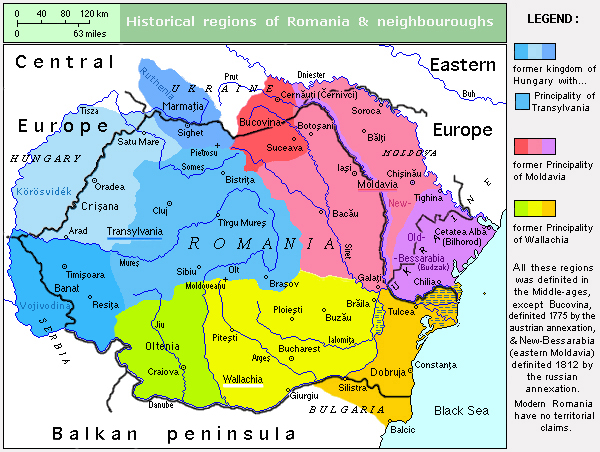
\includegraphics[width=13cm,height=9.5cm]{images/RomaniaHistRegions.jpg}
                \caption{Régions historiques de la Roumanie\footcite{pazdzioraHistoricalRegionsRomania2009}}
                \label{fig1}
            \end{figure}
		\vspace{-0.8cm}	    
		\section*{Une communauté au plus bas de l'échelle sociale}
		% Ajoute à la table des matières sans numérotation
		\addcontentsline{toc}{section}{Les Roms, au plus bas de l'échelle sociale}	    
		    Dès leur arrivée, les Roms déconcertent~: leur provenance est souvent incomprise\footnote{Ils sont souvent pris pour des Tatars ou des Égyptiens, d'où les termes \og{}\textit{gypsy}\fg{} et \og{}\textit{gitano}\fg{}.}. Leurs mœurs ne sont pas davantage appréciées et les caricatures vont pénétrer l'imaginaire collectif jusqu'à nos jours. Ils sont rapidement réduits et maintenus en esclavage, parfois même sans personnalité juridique (Valachie et Moldavie). Ailleurs, même lorsqu'ils disposent d'un statut plus libéral, ils font l'objet de persécutions, d'expulsions, de tentatives de sédentarisation forcée et, d'une manière générale, de rejet et discriminations\footcites(Voir~: )(){marushiakovaGypsySlaveryWallachia2013}[][pp.~13-65 et 69-85]{achimRomaRomanianHistory2004}{hancockPariahSyndromeAccount1987}{soulisGypsiesByzantineEmpire1961}{beckOriginsGipsySlavery1989}.
		    
		    Néanmoins, les Roms deviennent une main-d'œuvre indispensable et leur présence s'impose dans la société. Avec les Lumières et au \siecle{xix} siècle, l'esclavage est remis en cause, progressivement réformé et aboli de 1783 en Bucovine puis Bessarabie\footnote{Bucovine et Bessarabie font alors respectivement partie des Empires austro-hongrois et russe.} et aboli en 1861 en Roumanie, où la nouvelle constitution de 1918 confère la citoyenneté aux Roms. Dès lors, ils s'organisent (organisations nationales de 1933 à 1941), à l'instar des autres minorités. 

    		L'historiographie\footcites(Voir~: )()[][pp.~87-161]{achimRomaRomanianHistory2004}{anastasoaieRomaGypsiesHistory2003}{mateiNationalismPragmatismRoma2020} a montré que depuis leur libération de l'esclavage au milieu du \siecle{xix} siècle, et même pendant l'entre-deux-guerres, il n'y avait pas de politique tsigane à proprement parler en Roumanie. Dans la vie politique et l'opinion en général, il n'y avait pas de \og{}problème tsigane\fg{} au sens du \og{}problème juif\fg{} invoqué de manière croissante en Europe, y compris en Roumanie. Les Roms étaient plutôt traités comme une catégorie sociale. Aussi ils ne sont pas considérés comme une minorité du ressort de la juridiction du Commissariat général aux minorités (\textit{Comisariatul General al Minoritãþilor}), créé en 1938\footcite[][p.~163]{achimRomaRomanianHistory2004}. L'attention qui leur est portée comme un groupe ethnique distinct relevait davantage des domaines de la sociologie et de l'ethnographie de la période\footcite[Notamment~:  George Potra, \textit{Contribuţiuni la istoricul ţiganilor din România}, Ed. Fundatia Regele Carol I, 1939); Ion Chelcea, \textit{Ţiganii din România monografie etnografică}, Ed. Institutul Central de Statistică, 1944), citées par~:][]{anastasoaieRomaGypsiesHistory2003}, des recherches qui ont largement contribué à la connaissance de leur situation dans les décennies d'avant-guerre, notamment grâce au recensement de 1930\footcite[][pp.~163–167]{achimRomaRomanianHistory2004}. Ce dernier recense 262 501 personnes se déclarant d'origine tsigane (1,5 \%
            de la population roumaine). La communauté Rom peut sembler être en passe de s'intégrer de manière croissante au cours de cette décénie \footcite[][pp.~223–224]{internationalcommisionontheholocaustinromaniaFinalReport2005a}.
            
            Cependant, l'héritage de plusieurs siècles de persécutions et de préjugés reste prégnant et les Roms restent cantonnés au bas de l'échelle sociale. Le nomadisme, même s'il diminue, continue de représenter un problème pour les autorités, qui n'ont de cesse de l'entraver\footcite[Voir la collection de transcriptions d'archives des autorités~:][]{nastasaVolumeDocumentsGypsies2001}, comme pour une partie de la communauté elle-même\footcite{marushiakovaLetterStalinRoma2020}, qui y voit un frein à une assimilation plus rapide.
            
            Et cette altérité, même si elle est devenue \og{proche}\fg{} selon les termes de Viorel Achim\footcite{achimDeportationRromsTransnistrie2016}, sera instrumentalisée par les partisans de l’eugénisme et de la biopolitique émergeant au cours de cette même décennie\footcite{wedekindMATHEMATIZATIONHUMANBEING2010} et sera à l'origine des persécutions à venir.
            \pagebreak
            
            Le territoire et la population de la Roumanie de 1918 a doublé et la part des minorités (hongroise, allemande, juive, ukrainienne, russe et rom) a triplé pour atteindre 30\%, causant craintes pour l'unité de la nation et vives tensions entre communautés\footcite{sanduRoumanieVictoirePyrrhus2015,MajorityQuestionInterwar2020}. L'État s'engage dans une politique de \og{}romanisation\fg{}, qui s'accompagne de déplacements de populations d'\og{}étrangers\fg{} et de l'octroi de privilèges aux Roumains \og{}de souche\fg{}. À l'aube de la seconde guerre, le pays est en proie à une forte instabilité politique\footcites{zahariaViePolitiqueRoumanie1985,blasenNominationCabinetGoga2018} et ne peut s'opposer à la perte de territoires, arbitrée par l'Allemagne et ses alliés\footcite{haynesGermanyEstablishmentRomanian1999} (figure \ref{fig2}).
            
            Ce contexte permet au maréchal Ion Antonescu\footnote{Surnommé le \og{}Guide\fg{} (\og{}\textit{Conducător}\fg{}), chef de l'État roumain de septembre 1941 à août 1944.} d'accéder au pouvoir, où il mène une politique fasciste avec l'appui de l'Allemagne nazie. En août 1941, cette dernière lui confie la Transnistrie, qu'il utilise pour mener à bien son projet d'épuration ethnique \footcites{achimDeportationRromsTransnistrie2016,benjaminPolitiqueAntijuiveRegime2011}.
            
            \begin{figure}[!ht]
    		    \centering
                %\href{https://isurvived.org/Pictures_Isurvived/transnistria.gif}
                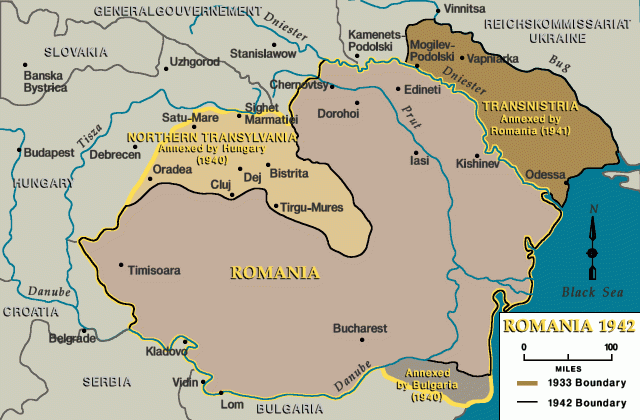
\includegraphics[width=12cm]{images/roumanie19331942.png}
                \caption{Évolution territoriale de la Roumanie lors du conflit\footcite{Romania1942}}
                \label{fig2}
            \end{figure}
        
        \pagebreak
        
        \section*{La déportation des Roms en Transnistrie}
	    % Ajoute à la table des matières sans numérotation
	    \addcontentsline{toc}{section}{La déportation des Roms en Transnistrie}
	    
	        Après avoir initié la déportation des juifs en 1941, le gouvernement du maréchal Antonescu décide d'entreprendre celle des Roms vers la Transnistrie\footcites[Quelques titres de référence détaillant la déportation des Roms :][]{achimRomaRomanianHistory2004,achimDeportationRromsTransnistrie2016,internationalcommisionontheholocaustinromaniaFinalReport2005a,aboutGenocidePersecutionRoma2016}.
	        
	        Le gouvernement a d'abord déporté tous les \og{}\textit{țiganii nenomazi}\fg{} recencés (Tsiganes nomades), soit 11\,441 personnes, à partir du 1\ier{} juin 1942 jusqu'au début de l'été 1942. 
                
            La déportation a ensuite été étendue en septembre 1942 à 13\,176 \og{}\textit{țiganii nenenomazi}\fg{} (Tsiganes non nomades) \og{}ayant un casier judiciaire, les récidivistes et ceux qui n'ont aucun moyen de subsistance et qui n'ont pas d'occupation définie leur permettant de subvenir à leurs besoins\fg{}. 
                
            Une troisième vague de déportations, préparée à l'automne 1942 pour le printemps 1943, fut remplacée par des déportations ponctuelles jusqu'en décembre 1943.
            \medskip
                
            Les conditions déplorables de voyage ou de transport et dans les camps, ainsi que les épidémies de typhus dues à la privation de nourriture et la violence des autorités roumaines, ont entraîné la mort d’environ 11\,500 personnes. Après la retraite de l’armée roumaine et le départ des autorités policières du gouvernorat de Transnistrie, la plupart des survivants sont rentrés en Roumanie au printemps 1944.

    	   \newpage

	\chapter[L'appariement des données~: état de l'art]{L'appariement des données~: état de l'art}
	
	\vspace{-0.5cm}
	\label{chap1}
	
		Pour analyser et reconstruire le parcours des Roms déportés, et en particulier pour en proposer une visualisation spatio-temporelle, le projet \og{}\textit{La déportation des Roms en Transnistrie, 1942 - 1944. Trajectoires individuelles, et destin collectif}\fg{} doit étudier le déplacement de ces populations sur la base de listes de personnes, établies en divers points des différents trajets. Ainsi il convient de lier, d'apparier le recensement initial des déportés de juillet 1942 avec les listes réalisées à l'embarquement dans les trains et ultérieurement au sein des camps d'internement, afin d'identifier de manière unique les personnes présentes dans plusieurs archives.
		
		Ce couplage de données permettra la consolidation au niveau individuel d'informations complémentaires, de les enrichir et, \textit{in fine}, de disposer de la vue d'ensemble nécessaire pour l'analyse des effets au long cours de ces persécutions.

		La tâche est aisée si les enregistrements disposent d’un identifiant unique dans les différentes sources. En revanche, le processus devient difficile en leur absence, en particulier lorsqu'il est confronté à des milliers d'enregistrements et des ensembles disparates.
		
		Dans l'étude de séries de sources, les manques et les incohérences des informations peuvent rendre leur mise en correspondance problématique. C'est d'autant plus vrai dans le cas des documents historiques car l'acquisition des données par des étapes de reconnaissance des caractères imprimés\footnote{\gls{ocr}} ou, à plus forte raison, d'écriture manuscrite\footnote{\gls{htr}}, introduit de nouvelles erreurs.
		\pagebreak

		\section{Historique et définition}
		    
		    \subsection{Définition}

			    Le couplage de données consiste à apparier des enregistrements (noms, dates de naissance, adresses et autres informations) provenant de différentes sources en une seule entité dans un seul fichier.
		    
		        De nombreux autres termes sont utilisés pour le qualifier comme rapprochement, appariement, fusion (informatique), recoupement (grand public), parfois liage de données, d'enregistrements ou encore de dossiers, de même que l'expression résolution d'entités\footnote{À distinguer de la Reconnaissance d'Entités Nommées (NER) ou \textit{Named Entity Recognition} (recherche d'entités nommées dans un texte et classement d'un point de vue sémantique~: personnes, lieux, entreprises, etc.). Toutefois, ces opérations sont parfois associées d'un point de vue technique et les auteurs emploient parfois ces terminologies de manière interchangeable.}...
		    
		        Dans une moindre mesure, cette variété se retrouve en anglais avec \textit{record linkage} (longtemps resté prédominant), \textit{data linkage/linking} ou \textit{data matching} (plus générique), \textit{deduplication}\footnote{Par abus de langage~: ce terme réfère au dédoublonnage au sein d'un même fichier.}. \textit{Record linkage} est désormais concurrencé par \textit{entity resolution/matching}.
		    
			\subsection{Historique}
			\label{historl}
			    La pratique des dénombrements et des recensements est multiséculaire\footcite{dupaquierHistoireDemographie1985}. L'intérêt pour une consolidation systématique d'informations issues de telles sources est également ancien et antérieur à l'apparition de l'informatique, notamment pour les sciences faisant appel aux statistiques, comme l'épidémiologie en médecine.
			    
			    Nous devons l'expression \textit{record linkage} à Halbert L. Dunn\footnote{Halbert Louis Dunn (1896-1975), médecin américain, a été l'un des fondateurs de la \textit{National Association for Public Health Statistics and Information Systems} (NAPHSIS) et de l'\textit{Inter-American Statistics Institute} (IASI).} en 1946~:
			    \og{}\textit{Each person in the world creates a Book of Life. This Book starts with birth and ends with death. Its pages are made up of the records of the principal events in life. Record linkage is the name given to the process of assembling the pages of this Book into a volume}\fg{}\footcite{dunnRecordLinkage1946}.
			    
			    Howard Newcombe\footcite{newcombeCouplageDonneesPour1969}, un des pères des bases théoriques du couplage d'enregistrements\footnote{Howard Borden Newcombe (1914-2005), généticien canadien, fut un pionner du \textit{record linkage}.}, voit déjà en William Farr un précurseur en ce domaine dès le \siecle{XIX} siècle (il fut directeur de la statistique au \textit{General Register Office}\footnote{William Farr (1807-1883), médecin épidémiologiste et statisticien britannique, est nommé en 1837 au \textit{General Register Office} chargé du recensement outre-Manche.}.
			    
			    Newcombe mentionne également les travaux en sociologie\footcite[Voir~:][]{christensenMethodRecordLinkage1958} de Christensen\footnote{Harold Taylor Christensen (1909-2003), professeur à l'université de Purdue (États-Unis), dont il fut le premier directeur du département de sociologie.} sur la famille aux États-Unis dès les années 30 et diverses autres études.
			    
			    En 1959, Newcombe contribue à jeter les bases de ce qui allait devenir les fondements des méthodes probabilistes en \textit{record linkage}\footcite{newcombeAutomaticLinkageVital1959}, formalisés de manière scientifique en 1969 par Ivan Fellegi et Alan Sunter\footcite{fellegiTheoryRecordLinkage1969}, une méthode toujours utilisée de nos jours.
			    
			    Avec l'avènement des techniques d'apprentissage automatique (\textit{Machine Learning}) dans les années 1990, ces méthodes sont affinées et améliorées avec l'introduction de comparaisons approximatives des chaînes de caractères entre des prénoms (Marie et Maria) ou des noms (Nicula et Nicolae)\footcites{christenDataMatchingConcepts2012,herzogDataQualityRecord2007a}, ou des techniques de segmentation des analyses sur les bases volumineuses (comparaisons de personnes du même sexe, du même lieu)\footcite{christenDataMatchingConcepts2012}.
			    
			    Récemment, les chercheurs ont créé des méthodes de comparaisons uniquement binaires (correspondances ou non-correspondances) basées sur un corpus d'entraînement, ainsi que des méthodes de regroupement (\textit{Clustering})\footcite{handNoteUsingFmeasure2018}.
			    
			    Enfin, les derniers développements s'intéressent~:
			    
			    \begin{itemize}
    			    \item
    			    aux méthodes de graphes\footcite{kirielleUnsupervisedGraphbasedEntity} (\textit{Graph}) pour caractériser les relations entres les entités afin d'utiliser ces nouvelles données dans le processus de couplage~;
    			    \item
    			    à l'apprentissage par transfert\footcite{kirielleTransERHomogeneousTransfer} (\textit{Transfer Learning}), qui permet de transposer des connaissances et des compétences acquises par un système lors de tâches antérieures sur de nouvelles tâches similaires, pour palier au manque de corpus d'entraînement pour ces modèles, pourtant de plus en plus performants~;
    			    \item
    			    aux problématiques de protection des données personnelles et procédés d'anonymisation\footcite{christenLinkingSensitiveData2021a}.
    			 \end{itemize}
			    
		\section{Vue d'ensemble/Principes généraux}
		
		    Nous nous intéressons principalement ici à l'appariement de personnes.
			    \subsection{Objectifs et terminologie}
			 
			    Dans le cadre de notre étude, l'objectif de l'appariement entre deux jeux (\textit{dataset}) de données individuelles, parfois nommées micro-données ou données très détaillées (\textit{microdata})\footnote{Par opposition aux données démographiques qui s'intéressent aux ensembles.}, est de déterminer si les paires (\textit{pairs}) de données de deux individus désignent la même personne.
			    
			    L'ensemble des paires possibles d'un dataset en est le produit cartésien, soit pour deux fichiers de taille \textit{n} et \textit{m}, le total des combinaisons est $n\times m$.
			    
			    Chacun des couples de données peut caractériser une paire d’individus identiques, auquel cas la paire est dite \textbf{liée} (\textit{match}), ou une paire d’individus différents, désignée comme \textbf{non liée} (\textit{unmatched / no match}). Les deux adjectifs \og{}lié\fg{} et \og{}non lié\fg{} correspondent aux résultats obtenus par le programme, le modèle ou l'outil utilisé pour qualifier les paires, sans lien avec le statut réel du résultat. Lorsque ce dernier est connu, \textit{i.e.} les données \textit{a} et \textit{b} d'une paire réfèrent effectivement au même individu, on parle de \textbf{paire annotée}, souvent après un contrôle ou une validation manuelle.
			    
			    L'appariement s'effectue grâce au degré de similitude entre les données disponibles dans les \textbf{variables} ou \textbf{attributs} (prénoms, noms, date de naissance, etc.) des disponibles dans les fichiers comparés.
			    
			    La comparaison peut être \textbf{exacte} (\textit{exact matching}) ou \textbf{floue} (\textit{approximate string comparison} ou \textit{fuzzy matching}). Dans le premier cas, une correspondance parfaite entre les données des attributs de la paire est requise pour obtenir une paire liée. Cependant, il existe souvent de nombreuses erreurs orthographiques, typographiques ou des variables manquantes dans les fichiers de micro-données individuelles. Il faut alors recourir à la deuxième méthode pour introduire une tolérance plus ou moins importante aux différences présentes dans les données, afin de pouvoir lier des paires qui ne seraient pas parfaitement correspondantes.
			    
			    \begin{table}[htbp]
                \begin{adjustbox}{width=1\textwidth,center=\textwidth}
                \Large
                \settowidth\rotheadsize{}
                \renewcommand\cellalign{cl}
                \renewcommand\arraystretch{2}
			        \begin{tabular}{|*{8}{c|}}
			        \hline
			            \multirow{2}{*}{}&\multicolumn{3}{c|}{Fichier 1}&\multicolumn{3}{c|}{Fichier 2}&Appariement\\ \cline{2-8}
                        \multirow{-2}{*}
                        {\diagbox[height=\rotheadsize + 3.9\line]
                        {\raisebox{0ex}{\shortstack{Type \\d'appariement}}}
                        {\raisebox{-0ex}{Données}
                        }}
                        &Prénom & Initiale & Nom & Prénom & Initiale & Nom & Résultat\\
                        \hline 
                        Exact&Ion&N.&Paslea&Ioan&&Paslae&\cellcolor{red!10!white}Paire non liée\\ \hline
                        Flou&Ion&N.&Paslea&Ioan&&Paslae&\cellcolor{green!10!white}Paire liée\\ \hline 
                    \end{tabular}
                    \end{adjustbox}
                \caption{Illustration de couplages exact et flou.}\label{tab1}
			    \end{table}
			 \pagebreak   
			 
			 \subsection{Étapes du processus de couplage}
			    Les principales étapes d’un processus d’appariement et les méthodes les plus communes qui leur sont associées sont les suivantes~:
			    
			    \begin{figure}[!ht]
                    \centering
                    \makebox[\textwidth]{
                        \begin{tikzpicture}[node distance =3cm, auto]
                        
                            % Place nodes
                            \node [block]                   (prep)  {\small{Analyse et préparation des données}};
                            \node [block, right of=prep]    (indexa)    {\small{Indexation}};
                            \node [block, right of=indexa]  (chps)  {\small{Analyse des champs}};
                            \node [block, right of=chps]    (paires) {\small{Classification}};
                            \node [block, right of=paires]  (conf)    {\small{Résolution des conflits}};
                            \node [block, right of=conf]    (qual)    {\small{Évaluation de la qualité}};
                        
                        \draw[line] (prep) -- (indexa);
                        \draw[line] (indexa) -- (chps);
                        \draw[line] (chps) -- (paires);
                        \draw[line] (paires) -- (conf);
                        \draw[line] (conf) -- (qual);
                        \end{tikzpicture}
                    }
                    \smallskip
                    \label{fig3}
                    \caption{Étapes des appariements}
                \end{figure}

			    \subsubsection{Standardisation et préparation}
			    Afin de tirer davantage d'information du traitement ultérieur des données, et notamment lors de la comparaison des chaînes de caractères, il convient dans un premier temps de les normaliser et standardiser, en identifiant et en traitant les points suivants.
			    
			    \begin{enumerate}
			        \item Les données non pertinentes~:\\
			        Au niveau des attributs, cela peut consister en la suppression de ceux sans utilité pour l'analyse (texte non structuré et complexe à analyser).
			        
			        Concernant les enregistrements, il s'agit notamment de supprimer les caractères spéciaux, la ponctuation, les diacritiques, la capitalisation des noms ou tout autre élément susceptible de causer davantage de bruit (\textit{noise}) qu'il n'apporte d'information. 
			        
			        Il est également nécessaire de s'assurer que les données pourront être exploitées. Si deux recensements listent l'âge des personnes (3 mois, 41 ans, 1 an, etc.), cette étape permet de transformer ces éléments variables (dans leur forme et dans le temps) par les valeurs fixes et stables comme l'année de naissance (soit, pour un document datant de 1942~: 1942, 1901, 1941, etc.).

			        \item Les données altérées ou inexactes~:\\
			        Des valeurs ou leurs combinaisons peuvent s'avérer inexactes ou contradictoires, par exemple un individu identifié comme un enfant mineur avec un âge de 32 ans ou encore un prénom mal orthographié en \og{}Cnostantin\fg{}. Lorsqu'elles sont indéniables, ces erreurs gagneraient à être corrigées, dans la mesure où la valeur correcte peut être déterminée. Préférer une analyse manuelle en excluant de tels enregistrements de l'analyse automatique peut également se révéler judicieux.
			        
			        \item Les données manquantes~:\\
			        De la même manière, il faudra arbitrer entre la suppression ou l'enrichissement en valeurs déduites pour des attributs ou des enregistrements qui seraient insuffisamment renseignés en fonction de l'importance de ces données pour le processus de couplage. Un exemple serait, sous certaines conditions, d'attribuer un genre masculin manquant à un individu prénommé \og{}Vladimir\fg{}. Il sera plus délicat de le faire pour \og{}Valerie\fg{}.
			        
			        \item La segmentation~:\\
			        Il peut s'avérer intéressant d'agréger (pour créer des clés de blocage, voir \ref{bloc}) ou de segmenter des informations (adresses avec numéro, nom de voie, code postal et ville) pour les rendre plus exploitables, en fonction des traitements de comparaison envisagés.
			        
			        Cependant, extraire les composantes, du nom d'un individu par exemple, peut nécessiter des règles codées complexes. Dans de nombreux cas de figures, ce processus implique la création et la maintenance de nombreuses tables de conversion. Pour palier à ces limites mais également obtenir une plus grande souplesse, des approches statistiques ce sont développées, notamment le modèle de Markov\footnote{Ou chaîne de Markow~: calcul de probabilité de phénomènes aléatoires basé sur le principe d'une interdépendance d'évènements liés les uns aux autres tels les maillons d’une chaîne, utilisé en reconnaissance vocable, l'analyse de séquences biologiques, le traitement automatique du langage naturel, etc.} (\textit{Hidden Markov Model}).

			        \item Les formats incompatibles~:\\
			        \label{format}
			        Pour pouvoir comparer les \textit{dataset} entre eux, le format de leurs attributs doivent être compatibles, notamment en ce qui concerne les chiffres (chaîne de caractères ou nombre), les dates, des coordonnées géographiques, etc..
			        Pour le genre des individus, un jeu de données disposant d'indicateurs F (féminin) ou M (masculin) ne saurait être directement comparé avec un autre, où les mêmes informations seraient codées \og{}\textit{Female}\fg{} et \og{}\textit{Male}\fg{}.
			    \end{enumerate}

			    L'importance de ces opérations de traitements en amont est nécessaire et souvent indispensable. L'objectif est double~: corriger ou supprimer les éléments qui pourraient nuire aux analyses et enrichir des modalités trop peu renseignées, afin de gagner en pertinence sans diminuer la valeur initiale des informations, un équilibre parfois délicat à trouver et qui peut induire la réalisation de différents tests.

			    \subsubsection{Indexation et blocage}
			    \label{bloc}
			    Nous avons vu que le nombre de paires est égal au carré de la dimension des bases à rapprocher. Pour deux sources de taille moyenne (10\,000 enregistrements), cela représente déjà 100 millions de couples possibles à analyser, ce qui est à la fois considérable et peu pertinent.
			    La proportion de paires d'individus uniques s'en trouve par ailleurs fortement diluée, ce qui représente un handicap dans la détermination des paires valides lors de la classification des paires liées et non liées.
			    Le principe de l'indexation est d'écarter en amont les paires indiscutablement incompatibles, du fait de nombreux attributs différents. Les stratégies de filtrage sont nombreuses, les plus importantes étant le \textbf{blocage} (\textit{blocking}) et les algorithmes de \og{}\textbf{voisins triés}\fg{} (\textit{Sorted Neighbourhood method ou SN}).
			    
			    \paragraph{Le blocage}\mbox{} \\
			    \label{blocking}
			    Cette méthode, très courante, vise à regrouper à l'avance les couples d'enregistrements les plus susceptibles d'être corrects (\textit{candidate pairs}). Dans l'hypothèse où les entités de deux sources devraient se situer dans la même zone géographique, il est possible d'utiliser le code postal comme \textbf{clé de blocage} (\textit{blocking key}), afin de ne comparer que celles qui sont géographiquement proches, diminuant ainsi drastiquement le nombre de comparaisons inutiles et les paires non liées.
			    
			    \begin{table}[htbp]
                \begin{adjustbox}{width=1\textwidth,center=\textwidth}
                \Large
                %\settowidth\rotheadsize{}
                \renewcommand\cellalign{cl}
                \renewcommand\arraystretch{2}
			        \begin{tabular}{|*{12}{c|}}
			        \hline
			            \multicolumn{6}{|c|}{Fichier 1 (gauche g)}&\multicolumn{6}{c|}{Fichier 2 (droite d)}\\
			            \hline
                        ID & Prénom & Nom & A. Naiss. & 
                        \Centerstack{ Code \\ résidence}
                        & Clé & ID & Prénom & Nom & A. Naiss. & \Centerstack{ Code \\ résidence} & Clé\\
                        \hline 
                        g1 & Ion&Paslea&1892&03001&ip03001& d1& I&Paslae&1939&03001&ip03001\\
                        \hline
                        g2 & Ion&Paslea&1915&03001&ip03001& d2&Ioan&Paslae&1915&03001&ip03001\\ \hline
                        g3 & Ion & Paslea & 1892 & 27003 & ip27003 & d3& Ion & Paslea & 1892 & 27003 & ip27003\\ \hline
                        g4 & Ionita & Paslea & & 03001 & ip03001 & d4& Ion & Paslea & 1892 && ip\\ \hline
                    \end{tabular}
                    \end{adjustbox}
                \caption{Example fictif de clé de blocage (initales et résidence).}\label{tab2}
			    \end{table}
			    
			    Dans la table 1.2 (où g1 = d4, g2 = d2, g3 = d3, g4 = d1), tous les individus (à l'exception de g3, d3 et d4) sont regroupés par la clé de blocage \og{}ip03001\fg{}.
			    
			    Cela permet de ne pas comparer l'enregistrement g1 avec d3 car il ne réside pas dans les communes d'intérêt dans notre hypothèse (pourtant, g1 et d3 auraient sans doute été liés). On observe les limites du blocage sur d4~: il ne sera pas comparé à g1 car l'attribut code résidence est manquant, alors qu'il s'agit de la même personne. C'est une des problématiques majeures du blocage~: les informations utilisées pour les clés doivent être de bonne qualité et pertinentes (un blocage sur un code géographique aura moins de sens si les personnes ont pu déménager entre les deux sources).
			    
			    Parmi les méthodes les plus utilisées pour constituer les clés de blocage, citons les codifications phonétiques de champs comme le \textit{Soundex}\footcite{Soundex2022} (prononciations anglo-saxones et ses variantes (\textit{Phonex}, \textit{Phonix}), le \textit{New York State Identification and Intelligence System} (NYSIIS), le \textit{Double Metaphone} (multilingue) ou le \textit{Fuzzy Soundex}\, qui permettent d'obtenir un code unique à utiliser comme clé couvrant diverses variations orthographiques\footcite[][pp.~74-81]{christenDataMatchingConcepts2012}.
			    
			    \paragraph{Les approches des voisins triés}\mbox{} \\
			    
			    Pour cette méthode, élaborée par Hernandez et Stolfo\footcite{hernandezRealworldDataDirty1998}, les deux sources sont au préalable concaténées dans un fichier unique, \textit{i.e.} la recherche des couplages consiste alors en une recherche de doublons.
			    Une clé est ensuite calculée à partir d'attributs pertinents pour regrouper les enregistrements par un simple tri effectué sur les clés. Une fenêtre glissante d'une taille prédéfinie balaie le fichier et analyse les références les unes après les autres, limitant ainsi le nombre de comparaisons\footcite[Voir les illustrations et les explications dans~:][pp.~9-11]{lehtiUnsupervisedDuplicateDetection2006}.
			    
			    Le concept du \textit{SN} a deux principaux inconvénients, d'une part sa grande dépendance à la qualité des attributs choisis au début de la clé car une erreur sur les premiers caractères éloignerait fortement les entrées lors du tri et ils ne seraient pas comparés. L'autre est la taille de fenêtre qui détermine combien de lignes sont comparées les unes aux autres. Si la taille est sous-dimensionnée, des vrais \textit{match} risquent d'être manqués. À l'inverse, avec une dimension trop importante, des rapprochements inutiles seront opérés, affectant potentiellement les performances du modèle. Pour l'améliorer, la réalisation de multiples passages sur des clés différentes ou l'ajustement dynamique de la taille de la fenêtre ont été proposées.
			    
			    \paragraph{Autres méthodes}\mbox{} \\
			    
			    D'autres méthodologies de recherche de motifs ont été développées sur ce sujet riche en innovations~:
			    \begin{enumerate}
			        \item l'indexation basée sur les mesures de \textit{n-grammes de caractères} (voir \ref{ngram}) ou de tableaux de suffixes~;
			        \item l'indexation par \textit{clustering} ou \textit{canopies}~;
			        \item les techniques d'indexation multidimensionnelle\footcite{kouahlaIndexationDansEspaces2013}.
			     \end{enumerate}
			   
			    Indispensable pour les fichiers volumineux, l'étape d’indexation vise à trouver un équilibre entre le coût du nombre de comparaisons à effectuer en termes de capacités computationnelles et de résultats, et la qualité de l’appariement final (une indexation drastique peut exclure des paires valides et créer de faux-négatifs).
			    
			    \subsubsection{Comparaison des champs}
			    \label{similarite}
			    Après l'optimisation de la recherche des paires par l'indexation vient la phase d'analyse des couples à apparier.
			    Dans la plupart des cas, un appariement exact ne permettra pas de lier les enregistrements en raison des erreurs et des variations présentes dans des sources qui n'ont souvent, ni été pensées, ni structurées comme de réels dossiers d'identification.
			    Ainsi des outils ont été développés pour effectuer des comparaisons approximatives prenant en compte les nuances induites par des collectes d'information non standardisées.
			    En évaluant le nombre de différences entre deux chaînes de caractères, ils permettent de calculer une mesure de distance et d'estimer le degré de similitude entre les deux données comparées.
			    
			    \paragraph{Distance de Levenshtein (ou distance d'édition)}\footcite{DistanceLevenshtein2022}\\
			    
                C'est la plus commune et elle se définit comme le nombre minimal d'insertions, de suppressions et de remplacements de caractères pour passer d'une chaîne à une autre~:
                
                    \begin{figure}[!ht]
                    \centering
                    \makebox[\textwidth]{
                        \begin{tikzpicture}[node distance =4.5cm, auto]
                        
                            % Place nodes
                            \node [block]                   (1)  {\small{Cnostantin}};
                            \node [block, right of=1]    (2)    {\small{C\textcolor{red}{\textbf{o}}ostantin}};
                            \node [block, right of=2]  (3)  {\small{Co\textcolor{red}{\textbf{n}}stantin}};
                            \node [block, right of=3]    (4) {\small{Constantin\textcolor{red}{\textbf{a}}}};

                        \path [line] (1) -- node [text width=3cm,midway,above,align=center ] {\scriptsize substitution} (2);
                        \path [line] (2) -- node [text width=3cm,midway,above,align=center ] {\scriptsize substitution} (3);
                        \path [line] (3) -- node [text width=3cm,midway,above,align=center ] {\scriptsize insertion} (4);

                        \draw [decorate,decoration={brace,amplitude=5pt,mirror,raise=2ex}](1.south west) -- (4.south east) node[midway,yshift=-3em]{Distance de Levenshtein (coût) = 3};
                        
                        \end{tikzpicture}
                    }
                    \label{fig4}
                    \caption{Calcul de la distance de Levenshtein.}
                \end{figure}
                
                Pour les appariements, un calcul de similarité est préféré. Il permet d'obtenir un indicateur entre 0 (pas de similarité) et 1 (correspondance exacte). Il est souvent normalisé (noté \textit{sim\textsubscript{Méthode}} ci-après), en le rapportant à la longueur de la plus grande chaîne, car une seule altération n'est pas équivalente selon la longueur des mots, soit dans notre exemple~:
                \bigskip
                
                Similarité normalisée \textit{sim\textsubscript{Levenshtein}}  = 1 - $ \dfrac{distance\,(3)}{longueur\,(Constantina~:\,11)} $ = 0,72.\\
                
                
                La mesure de \textbf{Damerau-Levenshtein}\footcite{DistanceDamerauLevenshtein2020} est une variante qui prend également en compte la permutation de caractères adjacents. Par conséquent, dans l'exemple ci-dessus, l'inversion des lettres o et n correspond à un changement au lieu de deux. Les distances de Damerau sont toujours inférieures ou égales à celles de Levenshtein (et les similarités plus fortes). Ici, \textit{sim\textsubscript{Damerau}} (Cnostantin, Constantina) = 0,82.
                
                \paragraph{Similarité de Jaro}\footcite{DistanceJaroWinkler2021}\\
                
                Basée sur le nombre et l’ordre des caractères communs entre les deux chaînes de caractères, elle a été notamment développée pour la détection de doublons de noms.
                
                \textit{sim\textsubscript{Jaro}} (Cnostantin, Constantina) = 0,936.
                
                
                \paragraph{Similarité de Jaro-Winkler}\footcite{DistanceJaroWinkler2021} \\
                
                Adaptation de la mesure précédente, elle est censée favoriser les chaînes les plus proches sur leurs premiers caractères, en partant du principe que les altérations sont plus fréquemment observées en fin de mot qu'au début.
                
                Ainsi, la position de certains changements sont neutres pour Levenshtein et Jaro~:
                \vspace{0.2cm}
                
                \textit{sim\textsubscript{Lev.}} (C\textcolor{red}{\textbf{no}}stantin, Constantina)  =  \textit{sim\textsubscript{Lev.}} (Constan\textcolor{red}{\textbf{it}}n, Constantina) = 0,72 et
                \vspace{0.2cm}
                
                \textit{sim\textsubscript{Jaro}} (C\textcolor{red}{\textbf{no}}stantin, Constantina)  =  \textit{sim\textsubscript{Jaro}} (Constan\textcolor{red}{\textbf{it}}n, Constantina) = 0,936.
                \newline
                
                En revanche, la similarité Jaro-Winkler pénalise davantage celles situées en début de chaîne, ainsi~:
                
                \textit{sim\textsubscript{JaroWinkler}} (C\textcolor{red}{\textbf{no}}stantin, Constantina) = 0,942 obtient un score moindre que~:
                \vspace{0.2cm}
                
                \textit{sim\textsubscript{JaroWinkler}} (Constan\textcolor{red}{\textbf{it}}n, Constantina) = 0,962.
                
                \paragraph{Smith–Waterman algorithm}\footcite{SmithWatermanAlgorithm2022} \\
                
                Développée à l'origine pour l'analyse de séquences en biologie (étude du génome par exemple), son principal intérêt en data matching est sa relative tolérance aux lacunes, qui rend cette méthodologie intéressante pour l'analyse de groupes de mots comportant des abréviations ou des initiales~:
                
                
                \textit{sim\textsubscript{Levenshtein}} (Gheorghe Dumitru Lacatus, Gh D Lacatus) = 0,5 et
                
                
                \textit{sim\textsubscript{JaroWinkler}} (Gheorghe Dumitru Lacatus, Gh D Lacatus) = 0,577,
                \newline
                tandis que~:
                
                \textit{sim\textsubscript{SimthWaterman}} (Gheorghe Dumitru Lacatus, Gh D Lacatus) = 0,67.
                \newline
                
                Cette mesure permet en outre d'associer des coûts ou scores particuliers aux différents types de mutations dans les chaînes, selon les besoins (voir la proposition au domaine des appariements par \hyperref[monge]{Monge et Elkan}).
                \newpage
                
                Ces approches sont relativement efficaces pour apparier en dépit des erreurs orthographiques mais elles sont en revanche très sensibles à l'ordre d'apparition des mots. Des chaînes pouvant être considérées comme liées ou valides obtiennent alors de faibles scores~:
                \smallskip
                
                \textit{sim\textsubscript{Levenshtein}} (Lacatus Gheorghe Dumitru, Gheorghe Dumitru Lacatus) = 0,33,
                \vspace{0.2cm}
                
                \textit{sim\textsubscript{JaroWinkler}} (Lacatus Gheorghe Dumitru, Gheorghe Dumitru Lacatus) = 0,70,
                \vspace{0.2cm}
                
                \textit{sim\textsubscript{SimthWaterman}} (Lacatus Gheorghe Dumitru, Gheorghe Dumitru Lacatus) = 0,33.
                
                
                \paragraph{Similarité basée sur les chaînes atomiques}\mbox{}\\
                \label{ngram}
                Pour remédier à ces limitations\footnote{Les distances d'édition ont d'autres inconvénients, comme l'absence de traitement sémantique, relevant d'autres domaines (traitement automatique des langues) que nous ne détaillerons pas ici.}, d'autres méthodes peuvent être mises en œuvre. Ces métriques, dites \og{}n-grammes\fg{} (\textit{n-grams})\footcite{Ngram2022}, analysent des sous-ensembles ou \og{}sacs\fg{} de \textit{n} mots (\textit{bags of words}) ou de \textit{n} caractères alphanumériques (\textit{tokens}) des chaînes. Dans le domaine du couplage, les plus fréquemment citées sont~:
                
                \subparagraph{Jaccard}\footcite{IndiceDistanceJaccard2021} \\
                
                La similarité de Jaccard calcule le rapport entre le nombre de \textit{n} sous-séquences en commun au nombre de toutes les sous-séquences de deux chaînes~:
                
                Au niveau des mots, entre \og{}Gheorghe Dumitru Lacatus\fg{} et \og{}Gh Dumitru Lacatus\fg{}, \textit{sim\textsubscript{Jaccard}} correspond à 2 (Dumitru et Lacatus en commun) sur 4 (Gheorghe, Gh, Dumitru et Lacatus), soit 0,5.
                
                Elle est peu adaptée aux chaînes courtes\footnote{Il existe des variantes qui peuvent corriger les limites du modèle de base.}, par exemple si l'on mesure les bigrammes communs de ioan (io, oa et an) et de ion (io et on)~:
                \vspace{0.2cm}
                \newline
                - la \textbf{distance de Jaccard} est alors~:
                \vspace{0.2cm}
                \newline
                \textit{dist\textsubscript{Jaccard}} (ioan, ion) = 1 - $ \dfrac{communs\,(io)}{total\, uniques\,(io, oa, an, on)} $ = 0,75.
                \newline
                \newline
                - l'\textbf{indice de Jaccard} est~:
                \bigskip
                \textit{sim\textsubscript{Jaccard}} (ioan, ion) = $ \dfrac{communs\,(io)}{total\,uniques\,(io, oa, an, on)} $ = 0,25.
                
                \newpage
                
                
                \subparagraph{TF-IDF (Token Frequency - Inverse Document Frequency) ou Cosinus}\footcite{TFIDF2022} \\
                
                Cette méthode est utilisée dans le domaine de recherche d’information, en particulier sur internet. En étudiant parallèlement les fréquences faibles et élevées de termes ou signes dans un corpus, elle permet de dégager ceux qui sont discriminants par contraste avec ceux qui sont très courants. Ainsi, un nom propre de société \og{}Orange\fg{}, moins commun, aura plus de poids dans le processus d'appariement que le terme \og{}société\fg{}.
                \newline
                
                Ces approches sont efficaces et rapides car elles sont basées sur des calculs relativement simples, notamment le calcul de Jaccard. Elles sont surtout adaptées à l'analyse de chaînes plus longues, comparativement aux mesures de distances, ainsi qu'aux larges corpus (dans le cas du TF-IDF, les poids des termes seront d'autant plus significatifs que le corpus est important). En revanche, les variations réduisent assez fortement leurs capacités de rapprochement.
                
                \paragraph{Mesures hybrides}\mbox{} \\
                
                Les mesures de distances comme les analyses n-grammes ont donc leurs limites. Aussi, pour tenter de combler leurs lacunes respectives, des combinaisons de plusieurs algorithmes ont été proposées pour affiner les modèles.
                
                \subparagraph{Monge-Elkan}\mbox{} \\
                \label{monge}
                
                La mesure de Monge-Elkan a été développée pour comparer de manière floue des chaînes de plusieurs mots (noms de sociétés, noms de personnes non segmentés).
                
                Chaque mot de la chaîne étudiée est comparé à ceux de la deuxième source par un calcul de similarité. En reprenant l'exemple \og{}Gheorghe Dumitru Lacatus\fg{} et \og{}Lacatus Gh Dumitru\fg{}~:
                
                \textit{sim\textsubscript{JaroWinkler}} (Gheorghe, Lacatus) = 0
                
                \textit{sim\textsubscript{JaroWinkler}} (Gheorghe, Gh) = \textbf{0,8}
                
                \textit{sim\textsubscript{JaroWinkler}} (Gheorghe, Dumitru) = 0,42

                \textit{sim\textsubscript{JaroWinkler}} (Dumitru, Lacatus) = 0,52
                
                \textit{sim\textsubscript{JaroWinkler}} (Dumitru, Gh) = 0
                
                \textit{sim\textsubscript{JaroWinkler}} (Dumitru, Dumitru) = \textbf{1}
                
                \textit{sim\textsubscript{JaroWinkler}} (Lacatus, Lacatus) = \textbf{1}
                
                \textit{sim\textsubscript{JaroWinkler}} (Lacatus, Gh) = 0
                
                \textit{sim\textsubscript{JaroWinkler}} (Lacatus, Dumitru) = 0,52
                \newpage
                
                Les meilleures combinaisons de paires générées sont donc Gheorges et Gh, Dumitru et Dumitru, Lacatus et Lacatus, dont on fait ensuite la moyenne.
                \vspace{0.2cm}
                \newline
                La similarité globale est \textit{sim\textsubscript{MongeElkan}} = $ \dfrac{1}{3} $ (0,8 + 1 + 1) = 0,93.
                \vspace{0.2cm}
                \newline
                À titre de comparaison, \textit{sim\textsubscript{JaroWinkler}} = 0,63.

                \subparagraph{Soft-Tf-idf}\mbox{} \\
                
                De la même manière, la méthode TD-IDF est combinée avec une mesure de distance approximative, tolérant les variations. Les fréquences et poids relatifs sont calculés sur un ensemble de mots dont certains sont considérés équivalents, au dessus d'un seuil de tolérance de similarité donné. 
                
                \paragraph{Distances phonétiques}\mbox{} \\
                
                Il est également possible d'être confronté à des données dont les variations orthographiques sont trop importantes pour être convenablement traitées par les analyses présentées jusqu'ici.
                
                \subparagraph{Editex}\mbox{} \\
                
                Nous évoquions l'intérêt du \textit{Soundex} pour le blocage (voir \ref{blocking}). Le \textit{Soundex} est un code alphanumérique de quatre caractères. Comme pour la distance de Levenshtein, l'\textit{Editex} permet de mesurer et d'attribuer un coût à un changement de prononciation. Il peut donc être pertinent dans l'analyse de chaînes courtes tels que les prénoms ou les noms, notamment pour atténuer les altérations de voyelles, qui ne sont pas codées dans le \textit{Soundex}~:
                
                \textit{sim\textsubscript{Levenshtein}} (Lixandru, Alexandru) = 0,67,
                
                \textit{sim\textsubscript{Editex}} (Lixandru, Alexandru) = 0,83.
                \vspace{0.2cm}
                \newline
                Cette propriété peut, à l'inverse, constituer un frein à la discrimination~:
                \vspace{0.2cm}
                
                \textit{sim\textsubscript{Levenshtein}} (Dimitri, Dumitra) = 0,71,
                
                \textit{sim\textsubscript{Editex}} (Dimitri, Dumitra) = 0,86.
                
                
                \subparagraph{Syllable Alignment Distance}\footcite[Voir :][p.~118]{christenDataMatchingConcepts2012}
                
                Le principe de cette méthode consiste à convertir les chaînes de caractères en séquences de syllabes et d'évaluer le nombre d'altérations à effectuer pour les faire correspondre, selon une méthodologie analogue à celle des calculs de distance et de similarité de Smith-Waterman (coûts variables selon les opérations).
                
                \paragraph{Autres méthodes de comparaisons}\mbox{} \\
                
                Parmi les autres approches de comparaison, nous proposons d'aborder brièvement les suivantes~:
                
                \begin{itemize}
                \setlength\itemsep{0.8em}
                    \item Les \textbf{plus longues sous-chaînes communes} ou \textit{Longest Common Sub-String} (LCS)\footcite{LongueSouschaineCommune2021}. Elles consistent à déterminer la plus longue suite de caractères communs aux chaînes et n'est pas dépendante de l'ordre des mots.
                    
                    \item Méthode des \og{}\textbf{co-occurrences}\fg{}\footcite{ananthakrishnaEliminatingFuzzyDuplicates2002a}. Elle cherche à rapprocher des termes que les mesures de distance ne parviendront pas à résoudre (\og{}United States of America\fg{} et \og{}USA\fg{}), ou à les dissocier (\og{}USA\fg{} et \og{}UK\fg{}, de distance proche) par des associations logiques~: \og{}United States of America\fg{} et \og{}USA\fg{} peuvent être associés car ils sont liés par des références redondantes (\og{}co-occurrence\fg{}) à leurs États (Pennsylvanie, Texas, etc.).
                    \label{graph}
                    \item Les \textbf{graphes} ou \textit{graph} appliqués à l'appariement\footcites{GraphMatchingMethod,onGroupLinkage2007,onSocialNetworkAnalysis2008}. Le concept est ici d'étudier des groupes d'individus ou des personnes dans leurs contextes (membres d'une famille, auteurs et leurs co-auteurs) afin de résoudre le problème de couplage d'homonymes ou de données très éparses et approximatives.
                    
                    \item Comparaison de données numériques (âges, numéros de voie, coordonnées géographiques, etc.)~:
                    
                    Après avoir standardisé les informations (voir \hyperref[format]{les formats}), plusieurs approches sont possibles. Ainsi, les éléments peuvent être évalués au format numérique, soit en calculant une différence absolue, soit en mesurant une différence relative en pourcentage entre les valeurs.
                    
                    Sinon, la mesure d'une distance textuelle sur la chaîne peut se révéler intéressante, notamment en cas d'information trop disparates.
                    
                    Concernant les adresses, il existe un certain nombre d'outils de codification géographiques et de calcul de distances qui permettront d'évaluer les correspondances\footcite[][p.~124 et pp.~208-211]{christenDataMatchingConcepts2012}.
                \end{itemize}
                \newpage
                
                La diversité des mesures présentées ici témoigne de la variété des cas de figures, des mutations et des irrégularités qui peuvent apparaître dans les données généralement traitées pour le couplage.
                Elles ont chacune leurs spécificités et leurs limites et correspondent souvent à des usages relativement délimités (efficacité sur des chaînes soit courtes, soit longues), d'où l'intérêt de les combiner dans certains cas.
                Néanmoins, elles permettent toutes de jauger la similarité des informations entre les attributs de différentes sources, de manière standardisée (scores entre 0 et 1 par exemple). Les données complexes deviennent plus comparables pour les étapes suivantes du processus d'appariement.
                
			    \subsubsection[Comparaison des paires ou \og{}classification\fg{}]{Comparaison des paires ou \og{}classification\fg{}\footcite[Voir~:][pp.~129-162]{christenDataMatchingConcepts2012}}
			    \label{compare}
			    Dans l'étape de classification, les scores de similarités sont évalués entre les paires candidates (susceptibles d'être réconciliées), afin de les départager entre paires liées, non liées et parfois paires incertaines (paires dont la classification n'a pu aboutir et qui doivent faire l'objet d'un traitement particulier, comme un examen manuel).
			    
			    \paragraph{Les variables de couplage (\textit{match keys})}\mbox{} \\
			    
			    Il convient dans un premier temps de déterminer quels attributs (quelles données) seront utilisés pour réaliser les rapprochements.
			    
			    Ce choix dépend de la qualité et du pouvoir discriminant des attributs qui seront choisis comme variables de couplage, avec de possibles répercussions sur la qualité de l'appariement.
			    
			    Comme pour le \hyperref[blocking]{blocage}, les variables de couplage sont des attributs pour lesquels les données sont fiables, relativement bien renseignées et discriminantes, invariables dans le temps (dates de naissance plutôt que l'âge).
			    Cette étape se nourrit de l'analyse des données de la phase de standardisation et de préparation, qui permet en outre de corriger ou d'inférer des informations erronées, altérées ou manquantes, par exemple à l'aide de dictionnaires de références.

			    La redondance d'information entre les variables est aussi à étudier, notamment pour des modèles d'appariement statistiques (voir ci-dessous)~: incorporer des données interdépendantes telles que ville et code postal peuvent affecter le poids relatif de la concordance (ou non concordance) de ces éléments dans l'évaluation des paires. Il est possible de corriger leur importance dans la classification ou de n'en utiliser la seconde que lorsque la première ne se révèle pas adéquate ou déterminante.
			    
			    Enfin, selon l'approche utilisée, cette étape doit enfin permettre d'évaluer le degré d'importance des variables entre elles car ces pondérations sont nécessaires dans certaines méthodes.
			    
			    \newpage
			    
			    Les logiques d'arbitrage dans la classification, en fonction des similarités obtenues, peuvent être extrêmement variées. Elles sont généralement regroupées au sein de deux catégories~:
			    
			    \paragraph{Les \textbf{méthodes déterministes}}\footcite[Voir des exemples dans le domaine de la santé~:][]{arielRecordLinkageHealth2015} \\
			    
			        Les classifications déterministes (\textit{deterministic} ou \textit{rules-based record linkage}) sont des méthodes \og{}locales\fg{}, \textit{i.e.} basées sur les éléments descriptifs des entités considérées indépendemment les unes des autres.
			        
			        Elles sont construites autour d'un ensemble de règles prédéfinies qui déterminent les décisions d'appariement, en fonction des similarités plus ou moins importantes entre les variables de couplage (attributs utilisés pour établir les liens).
			        
			        Intuitivement, la méthode la plus simple cherche à obtenir une correspondance exacte, par exemple des noms, prénoms, date de naissance et adresse afin d'établir qu'une paire est liée.
			        
			        Dans la réalité, les informations sont altérées et les règles doivent tenir compte des légères différences. Si les variables contiennent des erreurs, alors des paires liées ne pourront pas être appariées.
			        
			        Les approches déterministes induisent souvent la recherche d'un équilibre entre un matching parfait (\textit{full exact matching}) et une certaine tolérance aux variations des éléments (\textit{partial exact matching}).

    			    \begin{enumerate}
    			        \item  Méthode traditionnelle itérative~:
    			        
    			        La réconciliation des entités est effectuée en plusieurs étapes successives, utilisant en premier lieu des règles strictes (appariements exacts) puis en assouplissant les critères de correspondance (abandon de certaines variables, introduction de seuils de similarité dégressifs, etc.) sur les éléments les moins discriminants.
    			        
    			        Ces méthodes sont très intuitives et compréhensibles, économes en termes de temps de calcul. De plus, les paires liées à un stade du processus sont généralement exclues des itérations suivantes, limitant l'importance des opérations au fur et à mesure.
    			        
    			        Ce dernier point est l'une des principales limites du modèle~: une paire peut avoir été liée lors d'une des premières itérations du processus alors qu'un meilleur résultat aurait obtenu lors des rapprochements suivants.
    			        
    			        \pagebreak
    			        
    			        \item Méthodes basées sur la combinaison des similarités~:
    			        
    			        Contrairement à la technique précédente, celle-ci se veut non-itérative et son objectif est de combiner des seuils de similarité pour les variables étudiées, de les pondérer et de les agréger en un score global. En deçà d'un seuil de score global, les paires ne seront pas liées.
    			        
    			        Comme pour le processus itératif, sa mise en place est relativement aisée d'un point de vue technique. Elle est également économe en ressources informatiques.
    			        
    			        Néanmoins les règles sont délicates à déterminer, elles nécessitent une connaissance approfondie du domaine et souvent des essais itératifs pour jauger de leur efficacité à fournir une classification correcte des paires (qui peut être évaluée sur des échantillons dont le statut réel est connu).
    			        
    			        Afin de palier à cette difficulté, des adaptations de l'algorithme de Kuhn-Munkres (optimisation combinatoire des résultats pour obtenir le couplage parfait de poids optimum) ont notamment été proposées\footcites[Voir~:][]{}{guhaMergingResultsApproximate2004,AlgorithmeHongrois2022}.
    			        
    			    \end{enumerate}
			    
    			    En résumé, les méthodes déterministes sont nombreuses et variées car elles se prêtent bien aux projets d'appariement dédiés à un domaine de recherche particulier par leur flexibilité.
    			    
    			    Cependant, elles reposent souvent sur des observations empiriques et le choix des variables, des combinaisons de leurs résultats respectifs et la dégressivité des contraintes sont déterminantes~: comment évaluer un degré de similarité suffisant ?\footcite[Voir sur ce point la discussion dans~:][]{wangEntityMatchingHow2011}
    			    
    			    Les méthodes probabilistes ont pour objectif de déterminer de manière plus formelle et mathématique le pouvoir de discrimination des variables de couplage, en estimant la probabilité de leur (non) concordance dans les paires liées ou non liées.
			    \pagebreak
                \paragraph{Les \textbf{méthodes probabilistes}} (\textit{probabilistic record linkage})\footcite[][pp.~133-139]{christenDataMatchingConcepts2012}
			    
			    La plupart d'entre elles sont basées sur les travaux fondateurs de Fellegi et Sunter\footcite{fellegiTheoryRecordLinkage1969}.
			    
			    Dans ce modèle probabiliste, dit \og{}classique\fg{}, les paires sont classées entre paires liées, non liées et les paires indécises.
			    L'objectif est de minimiser la proportion de paires indécises, tout en contrôlant les taux d'erreurs dites de \og{}type I\fg{} et de \og{}type II\fg{} (respectivement taux de faux positifs et de faux négatifs).
			    
			    Dans ce modèle, le couplage optimal est atteint lorsque le nombre de paires indécises est faible et que les taux d'erreurs, ou de précision et de rappel\footcite{PrecisionRappel2022}, restent inférieurs aux taux spécifiés par l'opérateur.

			    L'intérêt de cette approche est qu'elle est applicable dans différents domaines et ne nécessite pas d'entraînement spécifique, n'a pas besoin d'apprentissage supervisé.
			    
			    Néanmoins, le modèle requiert une estimation des probabilités de (non) concordance dans les paires liées et non liées. Par exemple, la probabilité qu'un mois de naissance corresponde de manière fortuite dans des paires non liées est de 1 mois sur les douze mois de l'année. Les probabilités sont bien plus complexes sur les autres attributs.
			    Il faudra également paramétrer les taux d'erreurs et la nature des mesures de similarité.
			    Enfin, cette approche est basée sur l'hypothèse de l'indépendance entre les variables de couplage.
			    
			    Dans la réalité, il est fréquent que des attributs soient inter-dépendants (ville, code postal) ou que l'indexation ou la proportion des paires liées dans les données soit déséquilibrée, ce qui peut nuire à la qualité des résultats.
			    
			    De nombreuses recherches ont été menées pour pallier ces limites, comme la proposition de Winkler\footcite{winklerUsingEMAlgorithm2002} d'utiliser une méthode d'estimation des probabilités (algorithme espérance-maximisation\footcite{AlgorithmeEsperancemaximisation2022}) ou les travaux de Jaro\footcite{jaroAdvancesRecordLinkageMethodology1989}.
			    
			    Comme un appariement est une tâche binaire (lié, non lié), les recherches plus récentes se sont orientées vers l'apprentissage automatique (\textit{machine learning}) supervisé et non-supervisé pour classer les paires, ainsi que vers des méthodes de clustering.
			    \pagebreak
			    
			    \paragraph{Les \textbf{méthodes supervisées}} (\textit{supervised record linkage})\footcites[][]{pitaApplyingMachineLearning2017}[][pp.~:142-147]{christenDataMatchingConcepts2012}
			    
			    Ces méthodes permettent de construire des modèles qui apprennent à identifier de manière automatisée les meilleurs règles de classification, à partir d'échantillon de paires annotées, pour lier ou non les paires des datasets à réconcilier.
			    
			    Les plus communes sont basées sur la régression logistique (\textit{logistic regression}), les \textit{Support Vector Machines} (SVM)\footcite{MachineVecteursSupport2022} et les arbres de décision (\textit{random forest})\footcite{RandomForest2022} comme les \textit{Gradient Boosting Machines}\footcite{ApprentissageParRenforcement2022}.
			    
			    Leur grand intérêt est leur caractère automatique, cependant la nécessité de fournir des données annotées (le corpus d'entraînement) représente un frein. En effet, et notamment dans le domaine de l'appariement de données personnelles, il est relativement rare de disposer d'échantillons suffisamment adaptés aux cas de figure étudiés.
			    
			    Par ailleurs, ces modèles sont aussi sensibles à d'éventuels biais qu'il est souvent nécessaire de corriger, le plus souvent par une ou plusieurs phases d'apprentissage actif (\textit{active learning}), où les logiciels et programmes demandent aux opérateurs de classer des paires ambiguës pour affiner les règles de classifications.
			    
			    \paragraph{Les \textbf{méthodes non-supervisées}} (\textit{unsupervised record linkage})\footcite[][pp.~150-153]{christenDataMatchingConcepts2012}
			    
			    Pour ne pas avoir à fournir ou construire un corpus d'entraînement, des processus non-supervisés ont été développés.
			    
			    Ils sont basés sur les méthodes de clustering, en particulier le partitionnement en k-moyennes (\textit{k-means clustering})\footcite{Kmoyennes2022}, le clustering hiérarchique (\textit{hierarchical clustering})\footcite{RegroupementHierarchique2022} et l'espérance-maximisation (\textit{expectation-maximization})\footcite{AlgorithmeEsperancemaximisation2022} utilisée par Winkler.
			    
			    \paragraph{Les \textbf{méthodes relationnelles} ou méthodes globales}\footcite[][pp.~154-157]{christenDataMatchingConcepts2012}
			    
			    Ces techniques exploitent les relations des entités entre elles (liens familiaux) ou les contextes d'intervention (auteurs) pour aider la classification (voir \hyperref[graph]{les graphes}).
			    
			    \pagebreak
			    Au fil du temps et avec les développements informatiques, les méthodologies d'appariement ont évolué de démarches empiriques, vers des modèles statistiques et enfin vers des modèles mobilisant l'apprentissage automatique.
			    
			    Chacune d'elles se caractérise par ses avantages et inconvénients, de sorte que le choix d'un modèle relève à la fois des caractéristiques intrinsèques des données mais également de la nature du projet (compétence dans le domaine, ressources humaines et techniques, besoin ponctuel ou construction d'une chaîne de traitement pérenne).
			    
			    La distinction des modèles est d'ailleurs de moins en moins évidente et les recherches s'orientent vers une intégration progressive des techniques vers toujours davantage d'optimisation, que ce soit par l'apprentissage automatique dans la sélection des mesures de similarité ou de blocage ou l'introduction d'active learning dans de nombreux processus.

			    \subsubsection{Résolution des conflits}
			    
			    De nombreux systèmes de couplage réconcilient les paires une à une de manière indépendante, ce qui peut mener à des conflits~: cela peut se produire si des scores de similarité sont très proches entre plusieurs entités. Un autre cas de figure peut être le suivant~: si A est lié à B et que B est lié à C alors que A et C ont été classés comme une paire non liée, il faut résoudre les conflits.
			    
			    La manière la plus courante de résoudre les conflits fait appel à des algorithmes \og{}gloutons\fg{}, c'est à dire qui arbitrent de manière locale (au niveau des conflits) sans prendre en compte la qualité globale de l'ensemble des appariements.
			    
			    Pour une résolution plus globale qui cherche à optimiser la qualité globale des résultats de couplage, il faut faire appel à l'algorithme hongrois évoqué plus haut.
			    
			    \subsubsection{Évaluation de la qualité}
			    
			    Une fois le couplage effectué, il convient d'en évaluer la qualité d'une part, afin notamment de pouvoir prendre des mesures correctives s'il s'avérait insatisfaisant ou des pistes d'améliorations.
			    
			    Un premier indicateur sera le taux d'entités liées qui fournit une première évaluation globale l'efficacité de l'appariement.
			    
			    Si cette mesure peut être réalisée dans tous les cas, elle ne permet pas de juger de la pertinence des résultats.
			    \pagebreak

			    Pour évaluer la qualité du couplage\footcite[][pp.~163-184]{christenDataMatchingConcepts2012}, il est essentiel de savoir si les liens obtenus font en fait référence à la même entité, c'est-à-dire s'il s'agit de vrais liens. Si de vrais liens sont connus, le nombre de faux positifs (faux liens) et de faux négatifs (faux non-liens) peut être calculé, selon la \og{}matrice de confusion\fg{}~:
			    
			    \begin{table}[htbp]
                \begin{adjustbox}{width=1\textwidth,center=\textwidth}
                \settowidth\rotheadsize{}
                \renewcommand\cellalign{cl}
                \renewcommand\arraystretch{1.2}
			        \begin{tabular}{|c|c|c|c|}
			            \cline{3-4}
			            \multicolumn{2}{c}{}&\multicolumn{2}{|c|}{Statut réel}\\
			            \cline{3-4}
			            
                        \multicolumn{2}{c|}{}&Entités identiques (P) & Entités différentes (N)\\
                        \hline
                        \multirow{2}{*}{Statut prédit}&Lié (PP)&\cellcolor{green!10!white}Vrais positifs (VP)&\cellcolor{red!10!white}Faux positifs (FP)\\
                        \cline{2-4}
                        &Non lié (PN)&\cellcolor{red!10!white}Faux négatifs (FN)&\cellcolor{green!10!white}Vrais négatifs (VN)\\ \hline 
                    \end{tabular}
                    \end{adjustbox}
                \caption{matrice de confusion.}\label{tab3}
			    \end{table}
			    \vspace{-0.8em}
			    
			    Les indicateurs de qualité sont mesurés comme suit\footcite{SensitivitySpecificity2022}~:
			    \\
			    La qualité mesure les prédictions correctes sur l'ensemble des cas.
			    \vspace{0.8em}
			    
			    Qualité = $ \dfrac{\mbox{\textit{nombre de paires correctement classées}}}{\mbox{\textit{nombre total de paires}}} $ = $ \dfrac{VP + VN}{VP + VN + FP + FN} $
			    \newline
			    \newline
			    La précision (\textit{Precision}) évalue la part des prédictions correctes sur l'ensemble des prédictions positives, soit le pourcentage de réponses correctes, \textit{i.e.} si le modèle lie un seul cas juste, la précision est de 1. Cet indicateur à lui seul n'est pas suffisant.
			    \newline
			    
			    Précision = $ \dfrac{\mbox{\textit{nombre de paires liées correctement}}}{\mbox{\textit{nombre de paires liées par le modèle}}} $ = $ \dfrac{VP}{VP + FP} $
			    \newline
			    \newline
			    Le rappel (ou \textit{Recall}) quantifie les prédictions correctes sur l'ensemble des paires véritablement liées.
			    \newline
			    
			    Rappel = $ \dfrac{\mbox{\textit{nombre de paires liées correctement}}}{\mbox{\textit{nombre d'entités identiques}}} $ = $ \dfrac{VP}{VP + FN} $
			    \newline
			    
			    Précision et rappel doivent être analysés ensemble. Si l'objectif est de limiter le nombre de paires liées de manière erronée, il faut privilégier une meilleure précision, le modèle étant alors davantage sélectif. S'il s'agit de détecter plus de paires potentiellement correspondantes, l'accent doit porter sur un meilleur rappel.
			    
			    Enfin le F1-score (ou \textit{F1-measure}) est largement utilisé pour comparer les modèles entre eux (sur un même problème). Il correspond à la moyenne harmonique de la précision et du rappel, entre 0 et 1 (plus il est élevé, meilleurs sont les résultats). À titre indicatif, un F1-score de 50\% signifie que le modèle fait deux erreurs pour un vrai positif.
			    \newline
			    
			    F1-score = 2 x $ \dfrac{\mbox{\textit{Précision} x \textit{Rappel}}}{\mbox{\textit{Précision} + \textit{Rappel}}} $ = $ \dfrac{\mbox{2 \textit{VP}}}{\mbox{2 \textit{VP} + \textit{FP} + \textit{FN}}} $
			    \pagebreak
			    
			    En résumé, une meilleure précision peut se traduire par un faible rappel et inversement. L'indicateur le plus pertinent doit être favorisé aux regards des attentes, du niveau de risque accepté. De nombreux modèles permettent de régler ces paramètres afin que les résultats soient plus adaptés à la finalité de l'appariement, intimement liée à ces enjeux.
			    
		\section{Enjeux}
			 
			 Les enjeux sont nombreux et majeurs, tant pour le secteur public que le secteur privé.

			 Pour le secteur public, la médecine, en particulier l'épidémiologie, a été parmi les premiers secteurs pour lesquels il était crucial de rapprocher des informations, tant pour réaliser des études que pour assurer le suivi des patients. Nombre de projets et publications\footcites[Quelques exemples~:]{smithDataLinkageAustralia2021,sayersProbabilisticRecordLinkage2016,kirielleUnsupervisedGraphbasedEntity} relevant du \textit{record linkage} émanent de ce secteur\footnote{Notons que l'un des centres de recherches nationaux de santé publique en Angleterre dédié au \textit{data linkage} a été nommé le Farr Institute, d'après William Farr, pionnier du domaine (voir \hyperref[historl]{l'historique}).}.
			 
			 En matière de sécurité nationale et de police, le coupage des données devient primordial dans les processus de vérification d'identité et nécessaire dans le traitement, le suivi des affaires et leurs évaluations\footcite{shortRecordLinkageRoad2016,sadinleGeneralizedFellegiSunter2013}. C'est également vrai en prévention et détection de la fraude, comme pour l'identification des bénéficiaires effectifs d'avoirs fonciers et financiers.
			 
			 De même, la statistique publique a largement recours à ces technologies, avec pour enjeu la gestion administrative d'une part, et d'autre part les études statistiques et le suivi des politiques publiques dans de nombreux domaines\footcites{OutilAppariementIdentifiants}.
			 
			 Concernant les entreprises, les enjeux sont tout autant significatifs, à l'heure du développement du commerce mondialisé et de l'e-commerce. Dans des sphères très compétitives, connaître ses clients et fournisseurs est essentiel, nécessitant à la fois le nettoyage et la réconciliation, l'enrichissement et la protection des bases de données.
			 
			 Parallèlement, face à la profusion de données, notamment personnelles, les réglementations deviennent plus contraignantes et de nouvelles bonnes pratiques se développent.
			 \pagebreak
			 
		\section{Les appariements et la recherche}
			 
			 Avec la révolution informatique puis numérique des dernières décennies, des sources d'information plus exhaustives, plus diverses mais aussi plus dispersées sont devenues disponibles. La littérature scientifique témoigne de l'intérêt croissant des chercheurs pour l'exploitation de ces ressources, désormais permise par les progrès réalisés dans le traitement des données volumineuses, la modélisation et le traitement automatique.
			 
			 Ces sources, prises séparément, ont toutes leurs limites, que ce soient les données de panel susceptibles d'être biaisées ou les données administratives, fiables et disponibles sur le temps long, mais pauvres en informations relatives aux sujets de recherche.
			 
			 Le croisement de ces données a ouvert et continuera de renforcer la validité et la pertinence des travaux, notamment pour les études longitudinales. Le développement des techniques de couplage ont accompagné ces efforts, notamment aux États-Unis, au Canada, en Australie ou au Royaume-Uni.
			 \newline
			 
			 En France, qui dispose pourtant d'une information administrative riche, les acteurs constatent un retard relatif, notamment dû aux réglementations de protection des données en vigueur jusqu'à une époque récente\footcite[Lois Informatique et Libertés (1978) et sur l'obligation, la coordination et le secret en matière de statistiques (1951), avant les changement de 2004, 2008 et la loi pour une république numérique (2016)~:][]{picardAccesAuxDonnees2017}.
			 Pour palier cette situation, l'accès des données a été facilité par les réformes récentes et la mise en place du réseau Quertelet\footnote{\url{https://data.progedo.fr/} du TGIR Progedo \url{https://www.progedo.fr/}}, du Centre d'Accès Sécurisé Aux Données (CASD)\footnote{\url{https://www.casd.eu/}} et de la plateforme des données de santé (\og{}Health Data Hub\fg{})\footnote{\url{https://www.health-data-hub.fr/}}, notamment pour l'accès aux données sensibles.
			 \newline
			 
			 Concernant les archives historiques, signalons plusieurs projets récents ou en cours~:
			 
			 \begin{itemize}
			 \setlength\itemsep{0.8em}
			     \item le projet SOCFACE\footnote{Projet ANR-21-CE38-0013, \url{https://anr.fr/Projet-ANR-21-CE38-0013}}, de grande ampleur, qui vise à numériser analyser les recensements de 1836 à 1936 pour étudier les changement sociaux sur un siècle~;
			     
			     \item un autre projet ANR \og{}Qui est devenu un Nazi ?\fg{}, dont l'objectif est de créer une base de données des questionnaires de dénazification des zones d'occupation française et américaine en Allemagne (DeNazDB)\footnote{Projet ANR-21-FRAL-0005, \url{https://anr.fr/Projet-ANR-21-FRAL-0005}}~;
			     
			    \item le croisement du fichier central à d'autres sources, une expérimentation aux Archives Nationales\footcite{FichierCentralArchives}.
			 \end{itemize} 
			 \pagebreak
			 
			 En effet, grâce aux progrès des techniques de numérisation et d'acquisition des informations des archives, de nombreux corpus sont désormais accessibles à la recherche\footcite[Voir aussi le projet POPP de numérisation des recensements parisiens de l'entre-deux guerre~:][]{POPPProjetOcerisation}.
			 
			 Enfin dans des domaines légèrement différents, l'appariement géographique soutient le développement des référentiels géohistoriques tels que le \textit{Dictionnaire topographique de la France}\footnote{\url{https://dicotopo.cths.fr/}}, Paris Time Machine\footnote{\url{https://paris-timemachine.huma-num.fr/}}, ainsi que la consolidation de référentiels d'autorités en bibliothéconomie, comme les projets SudocAD\footcite{cheinSudocADKnowledgeBasedSystem2014}, repris par le projet ANR Qualinca\footcite[Projet ANR-12-CORD-0012, \url{https://anr.fr/Projet-ANR-12-CORD-0012~:} ][]{ObjectifsQUALINCA}.
		
		
    \pagestyle{empty}
	\cleardoublepage
	\pagestyle{plain}			
	
	\chapter[Mise en œuvre d'outils d'appariement]{Étude de l'appariement \\ \large des archives de la déportation des Roms}
		\label{chap2}
		
		Il sera question dans ce chapitre d'évaluer la faisabilité, le type de solutions à élaborer et leur rentabilité au regard des objectifs de la mission, en prenant en compte d'une part les caractéristiques des données sources, mais également le contexte organisationnel du projet. En outre, on discutera de la sélection des outils déployés pour répondre aux besoins.
	
		\section{Analyse des données}
			
			\subsection{Présentation générale des sources}
			
			    La collection numérisée\footcite{rg-25.050mSelectedRecordsVarious} comporte environ 25\,000 images issues, entre autres, des extraits des fonds des inspectorats généraux de gendarmerie et police, couvrant la majeure partie des listes nominatives de 25\,000 Roms visés par les mesures de persécution et de déportation.
			    
			    L’\gls{ushmm} a reçu la collection des Archives nationales roumaines (\textit{Arhivele Naţionale ale României}) au cours du projet d'archives internationales de l'\gls{ushmm} en décembre 2008 (microfilms 1-60) puis en mai 2010 (microfilms 61-64).
                
			    Il est important de noter que les listes sont produites à l’échelle locale : départements, villes et exceptionnellement inspectorats régionaux de gendarmerie ou de police. L'analyse portera donc sur ces évènements, département par département, pour les 62 départements contrôlés par le gouvernement Roumain en 1942 (en excluant la Transnistrie).

                \pagebreak
                
                \begin{figure}[!ht]
        			\centering
                    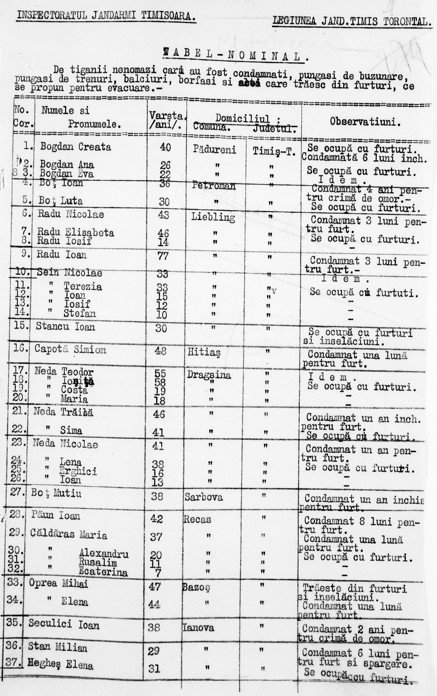
\includegraphics[width=11cm,height=12cm]{images/rg_25_050m_0010_00000344.jpg}
                    \caption{Exemple de liste nominative de proposition à la déportation\footcite[Liste de l'inspection de la gendarmerie de Timișoara~:][Copyright \textit{Arhivele Naţionale ale României}]{rg-25.050mfileid:45931SelectedRecordsVarious}.}
                    \label{fig5}
                \end{figure}
                \vspace{-2em}

			 \subsection{Des documents de qualité variable}
			    
			    Les listes ayant été établies par de très nombreux acteurs, leurs formes et leurs contenus sont très hétérogènes~:
			    
			    \begin{figure}[!ht]
        			\centering
                    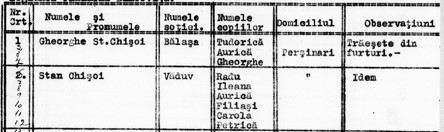
\includegraphics[width=11cm]{images/rg_25_050m_0010_00000502.jpg}
                    \caption{Liste par famille sur plusieurs colonnes, sans âges\footcite[][Copyright \textit{Arhivele Naţionale ale României}]{rg-25.050mfileid:45964SelectedRecordsVarious}.}
                    \label{fig6}
                \end{figure}
                %\vspace{-2em}
                \pagebreak

                \begin{figure}[!ht]
        			\centering
                    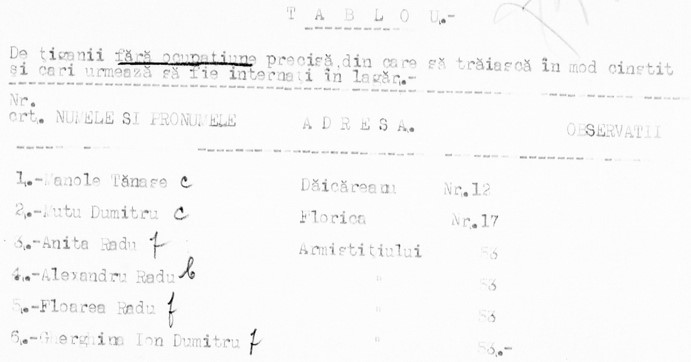
\includegraphics[width=13cm]{images/rg_25_050m_0010_00000803.jpg}
                    \caption{Liste sans indicateur de famille, sans âges\footcite[][Copyright \textit{Arhivele Naţionale ale României}]{rg-25.050mfileid:46036SelectedRecordsVarious}.}
                    \label{fig7}
                \end{figure}
                
                \begin{figure}[!ht]
        			\centering
                    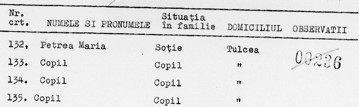
\includegraphics[width=13cm]{images/rg_25_050m_0012_00000204.jpg}
                    \caption[Liste avec des noms manquants]{Liste avec des noms manquants\footnote{\textit{Copil}, qui signifie enfant, est utilisé dans la colonne \textit{Numele si pronumele} (Noms et Prénoms).}, sans âges\footcite[][Copyright \textit{Arhivele Naţionale ale României}]{rg-25.050mfileid:46415SelectedRecordsVarious}.}
                    \label{fig8}
                \end{figure}
                
                \begin{figure}[!ht]
        			\centering
                    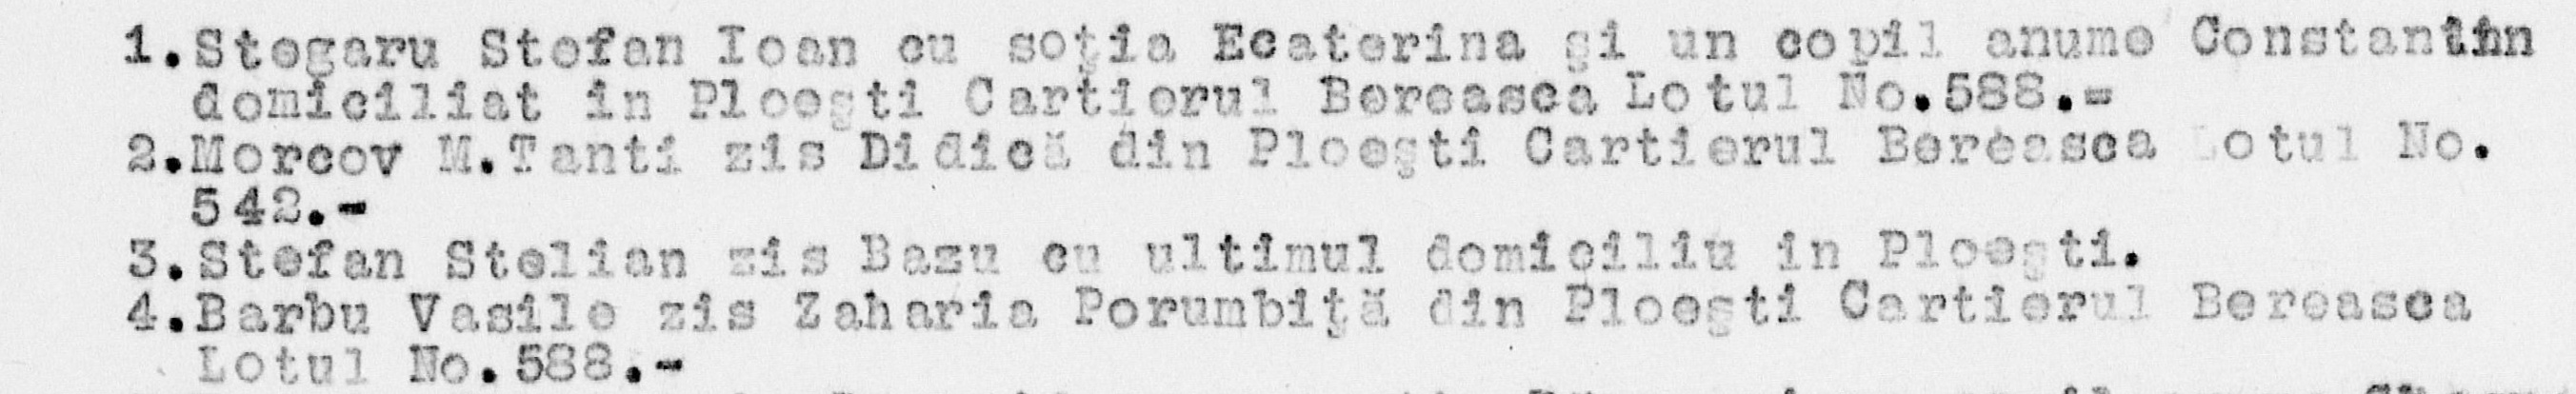
\includegraphics[width=13cm]{images/rg_25_050m_0012_00000534.jpg}
                    \caption{Liste non tabulaire, sans âges\footcite[][Copyright \textit{Arhivele Naţionale ale României}]{rg-25.050mfileid:46521SelectedRecordsVarious}.}
                    \label{fig9}
                \end{figure}
			    
			    \pagebreak
			    
			     La masse de données disponibles (125\,000 entrées individuelles pour environ 1\,500 documents) a induit, pour le chercheur, une analyse et une réconciliation des sources.
                
                Celle-ci a consisté à suivre les logiques et évènements administratifs afin de trier le corpus. L’\gls{ushmm} ayant inventorié et numéroté les différents dossiers d'archives, l’exploration de la documentation et de l’historiographie a permis d'en dégager les grandes lignes et identifier 1\,083 documents nominatifs.
                \newline

			    Les documents couvrent divers aspects de ces événements, notamment\footnote{Ainsi que divers autres documents sans liens directs avec la déportation.}~:
                \vspace{0.5em}
			    \begin{itemize}
			    %\setlength\itemsep{0.8em}
			        \item le recensement secret (mai 1942)~;
			        \item la déportation des Roms \og{}nomades\fg{} (juin - septembre 1942)~;
			        \item \underline{les listes des Roms \og{}sédentaires\fg{} sélectionnés pour la déportation (juillet 1942)}~;
			        \item \underline{les listes des Roms \og{}sédentaires\fg{} déportés (septembre 1942)}~;
			        \item \underline{les documents de transfert des Roms \og{}sédentaires\fg{} (septembre 1942)}~;
			        \item les évasions (1942-1944)~;
			        \item le recensement en préparation de la seconde déportation (octobre 1942)~;
			        \item le rapatriement des Roms mobilisés\footnote{En effet, certains Roms sont incorporés dans les forces armées du régime. La déportation concerne d'abord sur ceux qui ne l'étaient pas.}, déportés par erreur (1942-1943)~;
			        \item les listes des déportés dans les camps (1942-1943)~;
			        \item les déportations ponctuelles (1943)~;
			        \item les listes de rapatriés (avril - mai 1944)~;
			        \item des courriers de réclamation des déportés pour un rapatriement (1942-1944).
			    \end{itemize}
                \vspace{0.5em}
                
			    Cette phase du projet s'intéresse en particulier au rapprochement des listes soulignées ci-dessus, soit la pré-sélection des \textit{țiganii} \og{}sédentaires\fg{} de septembre 1942 et les départs effectifs à la fin du même mois, ainsi que l'organisation des trajets (voir la section \ref{parcours}), afin que le prestataire puisse réaliser un prototype de cartographie temporelle.
			    \newline
			    
			    En effet, le recensement de septembre fournit les adresses de départ, les listes à l'embarquement confirment la liste des personnes déportées, tandis que les documents de transport détaillent la répartition dans les trains et les trajets de ces derniers.
			    \newline
			    
			    De plus, le recensement et la déportation des Tsiganes \og{}sédentaires\fg{} constituent les épisodes pour lesquels les sources sont à la fois les plus exhaustives et les plus importantes.

			    Concrètement, le recensement de juillet concerne 18\,000 personnes et la déportation de septembre 13\,176 personnes, selon les documents du ministère de l’intérieur de 1942.
                \newline
                
			     Ces listes ont été transcrites par l'\gls{ushmm} et ses partenaires, puis préparées au format \acrshort{csv}, avec certaines métadonnées descriptives.
			     \pagebreak
			    
            \subsection[La source au format \glsentryshort{csv}]{Le fichier \acrshort{csv}}
            
            Par la suite, le recensement de septembre sera désigné régulièrement sous le terme de \og{}Census\fg{} et les données de la déportation sous celui de \og{}Déportation\fg{}\footnote{Par convenance et pour une meilleure analogie avec les noms des fichiers (census et deportation).}.
            
                \subsubsection{Le fichier global}
			    
                    Toutes les données de la première déportation sont fournies en un fichier \acrshort{csv} unique (133\,000 lignes environ), dont la structure est la suivante~:
    			    
    			    \begin{figure}[!ht]
            			\centering
                        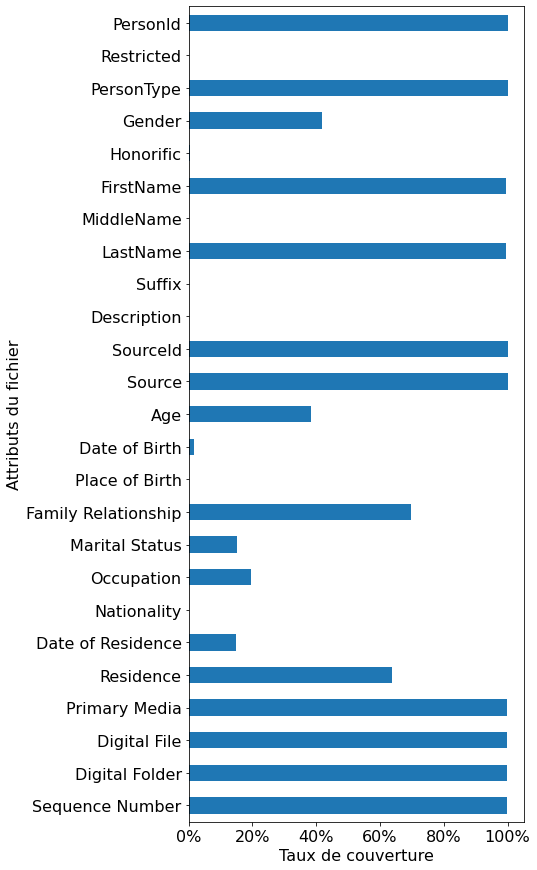
\includegraphics[width=11cm]{images/ushmm_content.png}
                        \vspace{-0.5em}
                        \caption{Structure de la source \acrshort{csv} (voir \hyperref[analyse1]{le code}).}
                        \label{fig10}
                    \end{figure}
    
    			    \pagebreak
    			    
    			    Après un examen détaillé, les attributs suivants ont être écartés~:
    			    
    			    %\vspace{0.8em}
    			    \begin{itemize}
    			    %\setlength\itemsep{0.8em}
    			        \item champs vides~: Restricted, MiddleName, Suffix, Description, Place of birth
    			        \item champs sans apport quantitatif ou qualitatif~: Honorific, Nationality
    			        \item métadonnées sans objet pour l'étude~: PersonType (\og{}\textit{Victim}\fg{} pour toutes les entrées), Primary Media (redondance avec Digital File).
    			    \end{itemize}
                    \vspace{-0.8em}

                \subsubsection{Les données relatives à la première déportation}
                
                    L'analyse des dossiers d'archives avait permis d'identifier que 317 d'entre eux portaient sur ces évènements, pour respectivement 21\,549 personnes recensées en septembre et 13\,033 répertoriées dans les listes de déportation\footnote{Sur la base du seul CSV, d'autres ont pu être identifiées et ajoutées manuellement~: toutes les sources n'étaient pas incluses et disponibles dans le fichier CSV.}. L'échantillon concerné par l'étude a par ailleurs le même taux de renseignement que le fichier complet~: 
                    \begin{figure}[!ht]
            			\centering
                        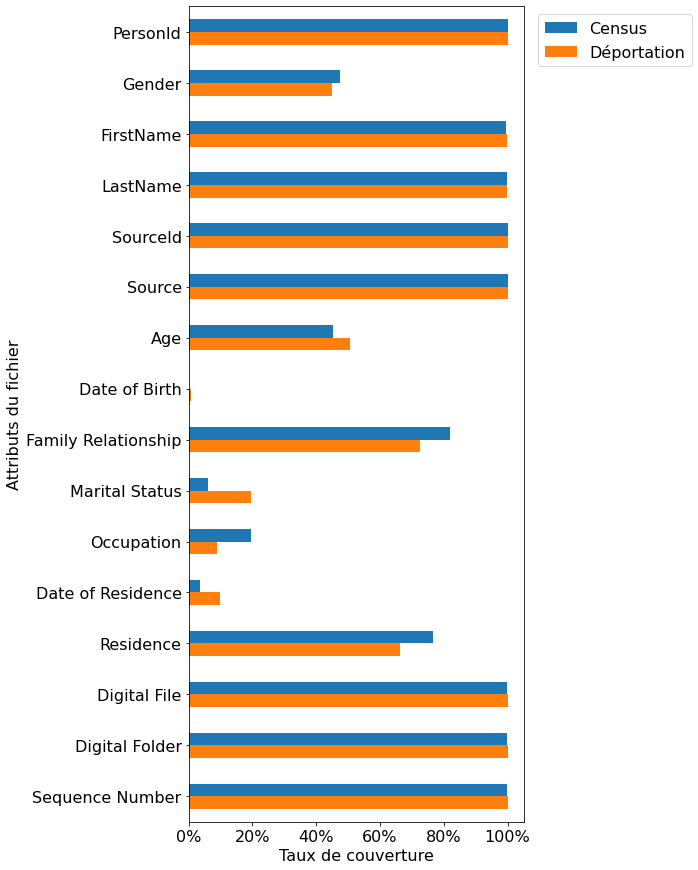
\includegraphics[width=12cm]{images/scope_content.png}
                        \caption{Structure confirmée sur l'échantillon de l'étude (voir \hyperref[analyse2]{le code}).}
                        \label{fig11}
                    \end{figure}
                    
                    \pagebreak
            
            \subsection{Analyse des attributs disponibles}
                    
                De fortes disparités de taux de couverture des attributs sont observés dans les fichiers, une analyse est nécessaire pour identifier ceux qui peuvent être utilisés pour l'étude, y compris pour évaluer la qualité des champs convenablement fournis en informations. En outre, lorsque des champs sont susceptibles de se compléter, ils sont étudiés ensemble.
                
                \subsubsection{Les données originales}
                
                \paragraph{Gender}\mbox{(Genre)} \\
                \label{genre}
                    Indicateur du genre des personnes, dont la détermination à partir les archives n’est pas toujours aisée, ce qui se reflète dans le taux de disponibilité insuffisant~:
                    \begin{itemize}
                        \item sur environ un quart des documents le genre est convenablement précisé~;
                        \item dans la moitié des documents, seul le genre des adultes est précisé soit via une colonne genre où les hommes sont étiquetés avec la lettre \og{}B\fg{} et les femmes avec la lettre \og{}F\fg{}, soit via le statut marital de mari et épouse~;
                        \item le genre des enfants, étiquetés avec la lettre \og{}C\fg{}, n'est qu'exceptionnellement précisé. Comme pour les adultes, le statut familial peut clarifier \og{}fils\fg{} ou \og{}fille\fg{}.
                    \end{itemize}
                    \medskip
                    
                    \begin{savenotes} % Pour traiter les footnotes dans tabular (+ package footnotes)
                    \begin{table}[ht]
                    \centering
                    \renewcommand\cellalign{cl}
                        \begin{tabular}{|c|c|c|}
                            \hline
                            Gender & \# Census & \# Déportation\\
                            \hline
                            Female &   7617 & 4014 \\
                            Male &   2610 & 1834 \\
                            NaN\footnote{\og{}NaN\fg{} signifie champs nul.} & 11322 & 7185 \\
                            \hline
                        \end{tabular}
                    \caption{Disponibilité du genre.}\label{tab4}
                    \end{table}
                    \end{savenotes}
                    
                L'absence de genre sur des entrées qui laissent pourtant peu de place au doute devrait permettre d'imputer certaines valeurs manquantes pour enrichir cet attribut.

                \paragraph{Family Relationship}\mbox{(Relation au chef de famille)} \\
                
                Indicateur reflétant la position des individus par rapport au chef de famille (homme ou femme), ce dernier étant noté \og{}\textit{Self}\fg{} (les célibataires peuvent également recevoir ce marqueur).
                En effet, lorsque les groupes familiaux sont décrits dans les listes (voir l'exemple suivant \ref{fig12}, mais également les figures \ref{fig6} et \ref{fig9}), le \acrshort{csv} reprend ces informations comme ci-dessous~:
                
                \pagebreak
                
                \begin{figure}[!ht]
        			\centering
                    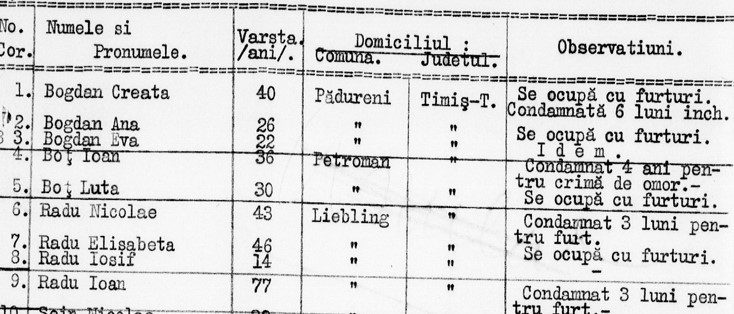
\includegraphics[width=13cm]{images/rg_25_050m_0010_00000344_detail.jpg}
                    \caption{Detail de liste\footcite[Liste de l'inspection de la gendarmerie de Timișoara~:][Copyright \textit{Arhivele Naţionale ale României}]{rg-25.050mfileid:45931SelectedRecordsVarious}.}
                    \label{fig12}
                \end{figure}
                \vspace{-2em}
                
                \begin{savenotes} % Pour traiter les footnotes dans tabular (+ package footnotes)
                \begin{table}[ht]
                    \begin{adjustbox}{width=1.1\textwidth,center=\textwidth}
                    \large
                    %\settowidth\rotheadsize{}
                    \renewcommand\cellalign{cl}
                    \renewcommand\arraystretch{2}
                    \renewcommand\cellalign{cl}
                        \begin{tabular}{c|c|c|c|c|c|c|c|c|c|c}
                            \cline{2-10}
& PersonId & \Centerstack{Gender\\
\footnote{Ici, le genre n'est pas renseigné ni par le code de lettres \og{}B\fg{}, \og{}F\fg{}, \og{}C\fg{}, ni par le statut familial (uniquement \og{}Self\fg{}, neutre).}} & \Centerstack{First\\Name} & \Centerstack{Last\\Name} & Age &  \Centerstack{Family\\ Relationship} & \Centerstack{Marital \\Status} & Residence & \Centerstack{Sequence \\Number}\\
\cline{2-10}
& 8768310 &  & Creata & Bogdan & 40 & Self &  & \Centerstack{Pădureni,\\Timiş-T.} & 1000 &\\
\cline{2-10}
+1\footnote{Incrémentation unitaire pour chaque personne, de haut en bas, de gauche à droite le cas échéant.}
& 8768311 &  & Ana & Bogdan & 26 &  &  & \Centerstack{Pădureni,\\Timiş-T.} & 1010 & +10
\footnote{Incrémentation par dix pour chaque personne, de haut en bas, de gauche à droite le cas échéant.}\\
\cline{2-10}
+1 & 8768312 &  & Eva & Bogdan & 22 &  &  & \Centerstack{Pădureni,\\Timiş-T.} & 1020 & +10\\
\cline{2-10}
+1 & 8768313 &  & Ioan & Boţ & 36 & \footnote{Ici, \og{}Self\fg{} manquant.} &  & \Centerstack{Pădureni,\\Timiş-T.\footnote{\label{note1}La transcription est erronée~: la ville aurait dû être Petroman.}} & 1030 & +10\\
\cline{2-10}
+1 & 8768314 &  & Luta & Boţ & 30 &  &  & \Centerstack{Pădureni,\\Timiş-T.\footref{note1}} & 1040 & +10\\
\cline{2-10}
+1 & 8768315 &  & Nicolae & Radu & 43 & Self &  & \Centerstack{Liebling,\\Timiş-T.} & 1050 & +10\\
\cline{2-10}
+1 & 8768316 &  & Elisabeta & Radu & 46 &  &  & \Centerstack{Liebling,\\Timiş-T.} & 1060 & +10\\
\cline{2-10}
+1 & 8768317 &  & Iosif & Radu & 14 &  &  & \Centerstack{Liebling,\\Timiş-T.} & 1070 & +10\\
\cline{2-10}
+1 & 8768318 &  & Ioan & Radu & 77 & Self &  & \Centerstack{Liebling,\\Timiş-T.} & 1080 & +10\\
\cline{2-10}
                        \end{tabular}
                    \end{adjustbox}
                \caption{La transcription CSV du document en figure \ref{fig12}}\label{tab5}
                \end{table}
                \end{savenotes}
                
                \pagebreak
                Les valeurs possibles pour le statut familial sont~:
                
                \begin{table}[ht]
                    \centering
                    \renewcommand\cellalign{cl}
                        \begin{tabular}{|c|c|c|}
                            \hline
                            Valeur & \# Census & \# Déportation\\\hline
                            Self & 6283 & 3301 \\\hline
                            Child & 6123 & 3547 \\\hline
                            NaN & 3902 & 3578 \\\hline
                            Wife & 2671 & 1048 \\\hline
                            Daughter & 1844 & 1048 \\\hline
                            Relative & 171 & 53 \\\hline
                            Concubine & 166 & 83 \\\hline
                            Spouse &  156 & 156 \\\hline
                            Husband & 87 & 0 \\\hline
                            Mother & 57 & 40 \\\hline
                            Brother & 20 & 32 \\\hline
                            Sister & 19 & 12 \\\hline
                            Relative-in-law & 17 & 23 \\\hline
                            Other & 0 & 22 \\\hline
                            Grandchild & 16 & 41 \\\hline
                            Other & 5 & 12 \\\hline
                            Relative-in-Law & 4 & 7 \\\hline 
                            Granddaughter & 4 & 32 \\\hline
                            Son & 0 & 7 \\\hline
                            Father &    2 & 3 \\\hline
                            Sibling &    0 & 3 \\\hline
                            Grandmother & 1 & 0 \\\hline
                            Grandfather & 1 & 1 \\\hline
                            relative & 0 & 2 \\\hline
                            Aunt & 0 & 1 \\\hline  
                        \end{tabular}
                \caption{Distribution des entrées de statut familial.}\label{tab6}
                \end{table}
                
                La forte disparité, avec des entrées anecdotiques (\og{}Aunt\fg{}) et des redondances (comme \og{}Spouse\fg{} et \og{}Wife\fg{}) induiront une standardisation de cet attribut, en particulier si l'on envisage de l'utiliser dans des règles d'appariement.
                
                \paragraph{Marital Status}\mbox{(Statut marital)} \\
                
                Champs complémentaire des deux précédents, il décrit le statut marital des intéressés, avec trois valeurs possibles uniquement~: \og{}Married\fg{} - marié(e), \og{}Widowed\fg{} - veuf(ve) - et \og{}Single\fg{} - célibataire.
                
                Les deux tableaux suivants analysent l'interdépendance de ces trois derniers attributs~:
                
                \pagebreak
                
                \begin{table}[ht]
                    \centering
                    \renewcommand\cellalign{cl}
                        \begin{tabular}{|c|c|c|c|}
                            \hline
                            \multicolumn{4}{|c|}{Census} \\
                            \hline
                            Gender & Family Relationship & Marital Status & Nombre \\\hline
                            Female & Wife & NaN & 2276 \\
                            Female & Daughter & NaN & 1830 \\
                            Female & NaN & NaN & 1124 \\
                            Female & Child & NaN & 1054 \\
                            Female & Wife & Married & 393 \\
                            Female & Self & NaN & 391 \\\hline
                            Male & Self & NaN & 1957 \\\hline
                            NaN & Child & NaN & 4893 \\
                            NaN & Self & NaN & 3206 \\
                            NaN & NaN & NaN & 2525 \\\hline
                        \end{tabular}
                    \caption[Correspondance de trois attributs Census]{Correspondance de trois attributs (Census)\footnotemark}\label{tab7}
                \end{table}
                \footnotetext{Les dix plus importantes quantités, voir l'analyse complète en annexe \ref{analyse4}.}
                
                \begin{table}[ht]
                \centering
                \renewcommand\cellalign{cl}
                    \begin{tabular}{|c|c|c|c|}
                        \hline
                        \multicolumn{4}{|c|}{Déportation} \\
                        \hline
                        Gender & Family Relationship & Marital Status & Nombre \\\hline
                        Female & Daughter & NaN & 1046 \\
                        Female & Wife & Married & 905 \\
                        Female & NaN & NaN & 522 \\
                        Female & Child & NaN & 374 \\\hline
                        Male & Self & Married & 789 \\
                        Male & Self & NaN & 454 \\
                        Male & Child & NaN & 281 \\\hline
                        NaN & Child & NaN & 2886 \\
                        NaN & NaN & NaN & 2705 \\
                        NaN & Self & NaN & 1175 \\\hline
                    \end{tabular}
                    \caption[Correspondance de trois attributs Déportation]{Correspondance de trois attributs (Déportation)\footnotemark}\label{tab8}
                \end{table}
                \footnotetext{Id., voir l'analyse complète en annexe au tableau \ref{tab8bis}.}
                
                Il ressort de l'analyse que très peu de valeurs~:
                \begin{itemize}
                    \item se contredisent~;
                    \item permettraient de déduire le genre à partir des deux autres variables, étant que la plupart des genres non renseignés sont associés à statuts familiaux neutres, de type \og{}Self\fg{} ou \og{}Child\fg{}~;
                \end{itemize}
                confirmant que le genre devra être déduit des prénoms, là où cela est possible.
                
                \paragraph{FirstName}\mbox{(Prénom)} \\
                
                Prénom ou prénoms (\textit{pronumele}) des personnes. Le champs \og{}MiddleName\fg{} n'ayant pas été utilisé, certaines entrées sont relativement complexes. Ces entrées doivent être analysées avec le nom, notamment parce qu'il est nécessaire de tenir compte des spécificités de la formation des noms en Roumanie.
                \pagebreak

                \paragraph{LastName}\mbox{(Nom de famille, Patronyme)} \\
                
                Nom(s) de famille (\textit{numele}) des personnes. Comme pour les prénoms, plusieurs caractéristiques influent sur les données retenues et répertoriées.
                
                \subparagraph{Note sur les données personnelles dans le contexte du projet}\mbox{} \\
                \label{spec_noms}
                Au moment où ces données sont produites, l’identité civile et l’identification restent largement floues en Roumanie.
                Ainsi, de nombreuses personnes peuvent être désignées par leur prénom et leur véritable patronyme mais aussi par l'association de leur prénom avec le prénom du parent (en général du père), voire les deux.
                
                En outre, il convient de souligner que certaines dénominations sont parfaitement interchangeables, avec des prénoms mixtes et d'autres très utilisés en tant que patronymes et inversement.
                
                En résumé, nous retrouvons ici l'éventail des difficultés évoquées par Peter Christen\footcite{christenComparisonPersonalName2006} pour ce type de données~:
                \vspace{0.8em}
                \begin{itemize}
                    \item variantes orthographiques, qu'elles soient issues de variantes réelles dans les graphies possibles (\textit{Ioan} et \textit{Ion}) ou d'erreurs (\textit{Anexandru} pour \textit{Alexandru})~;
                    \item variations phonétiques, résultant sans doute d'un enregistrement effectué oralement, avec des prononciations proches mais des orthographes relativement distinctes~;
                    \item des appellations alternatives, notamment des diminutifs (\textit{Veta} pour \textit{Elisabeta}) ou des surnoms (\textit{Alexandru zis Romica} pour \og{}Alexandru, dit Romica\fg{})~;
                    \item l'emploi d'initiales, relativement fréquentes dans le corpus.
                \end{itemize}
                \vspace{0.8em}
                Dans la documentation de la déportation des Roms, et en dehors des nuances culturelles indiquées plus haut, peuvent s'ajouter les écueils suivants~:\vspace{0.8em}
                \begin{itemize}
                    \item l'agrégation de divers prénoms et noms~;
                    \item l'ordre prénom - nom inversé~;
                    \item les abréviations des informations, causées notamment par l'espace restreint induit par le caractère tabulaire de l'enregistrement  (\textit{Ctin} et \textit{Constantin})~;
                    \item les erreurs liées au mauvais placement des signes de répétition dans les tableaux~;
                    \item les ratures et reprises.
                \end{itemize}
                \vspace{0.8em}
                Ces déformations sont exacerbées par l'état de conservation de certains documents, ainsi que par l'étape de transcription, qui a introduit de nouvelles variations ou confusions.
                \pagebreak

                \paragraph{Age}\mbox{(Âge)} \\
                
                L'âge des individus, généralement en chiffres, à l'exception des enfants de moins de un an, noté~: \og{}1/12 [1]\fg{} pour 1 mois. Par ailleurs, les documents ne datant pas tous de la même année, cette information est variable dans le temps, ce qui nécessitera une standardisation.
                
                Sur la donnée elle-même, les rapprochements préliminaires révèlent de possibles approximations (de l'ordre de plus ou moins trois à cinq ans), plus importantes pour les personnes âgées (parfois jusqu'à dix ans).
                
                \paragraph{Date of Birth}\mbox{(Date de naissance)} \\
                \label{age_desc}
                L'année de naissance des personnes (4 chiffres), très peu renseignée (50 sur le périmètre de l'étude). Une variable qui ne pourra pas être utilisée pour le rapprochement en l'état, mais qui peut être enrichie à partir de celle des âges.
                
                \paragraph{Occupation}\mbox{(Emploi)} \\
                
                Emploi ou catégorie d'activité, ce champs relativement peu complété fournit des informations très variables sur le statut des personnes, de la profession à la situation militaire (mobilisé ou non) ou judiciaire (condamnations), etc.. En dehors des notes concernant la mobilisation qui permet en partie de reconstituer les sélections de populations réalisées en 1942, cette variable est difficilement exploitable pour l'appariement, mais elle peut être intéressante pour le volet ethnographique de la recherche.

                \paragraph{Residence}\mbox{(Adresse)} \\
                
                Les adresses des personnes enregistrées, souvent limitées au lieu-dit ou village, avec parfois des adresses complètes en ville, le département (\textit{județ}) étant souvent mentionné.
                
                Cette donnée est affectée par des variations orthographiques du même ordre que les noms et prénoms, dont nous livrons un exemple ci-dessous.
                
                Cette variable a d'ailleurs fait l'objet d'une standardisation et un identifiant alphanumérique a été attribué aux différents lieux. Elle a également été enrichie lorsque cela était possible, avec les informations présentes au niveau des dossiers. C'est cette dernière donnée que nous utiliserons par la suite.
                
                \pagebreak
                
                \begin{table}[ht]
                \centering
                \renewcommand\cellalign{cl}
                    \begin{tabular}{|c|}
                        \hline
                        Adresse\\\hline
                        Tăndărei, Ialomiţa\\
                        Tăndărei, Ialomiţa || Galaţi\\
                        Tămdărei-Ialomiţa\\
                        Toudarei, Ialomita\\
                        Taudarei, Ialomita\\
                        Tăuderei, Ialomita\\
                        Tandarei, Ialomița\\
                        Tanderei, Ialomița\\
                        Tandarei, Ialomiţa\\
                        Tăndarei, Ialomița\\
                        Tanadrei, Ialomița\\\
                        Tândărei, Ialomița\\
                        Tăndărei, Ialomiță || Tăndărei, Ialomiță\\
                        Tăndărei\\
                        Tăndărei, Salomița\\
                        Tandărei\\
                        Tandărei || Galaţi\\
                        Tăndarei\\
                        Tândarei\\
                        Tandarei\\
                        Tănlărei\\
                        Tăniărei\\
                        Ţăndărei\\
                        Ţăndărei, Ialomiţa\\
                        Ţăndărei, Ialomiţ\\
                        Ţăndărei, Ialomita\\\hline
                    \end{tabular}
                    \caption{Différentes graphies d'un lieu de résidence.}\label{tab9}
                \end{table}
                
                \subsubsection{Les métadonnées}
                
                En ce qui concerne l'appariement, les deux variables les plus importantes sont les deux suivantes~:
                
                \paragraph{PersonId}\mbox{(Identifiant individuel)} \\

                Numéro de 7 chiffres attribué aux personnes (voir l'exemple au tableau \ref{tab5}), \og{}unique\fg{} si ces dernières ne sont pas mentionnées à différentes reprises dans une ou plusieurs sources.
                
                Cet identifiant permettra de constituer les identifiants des personnes et de les lier dans les bases de données, une fois l'appariement réalisé.
                \pagebreak
                
                \paragraph{Sequence number}\mbox{(Numéro de séquence)} \\
                
                Un code numérique (4 chiffres) identifiant l'ordre d'apparition d'une personne dans une liste, en principe de haut en bas pour les lignes, de gauche à droite à l'intérieur d'une ligne, d'un bloc d'information. La première personne reçoit le chiffre 1000, qui est incrémenté de dix en dix le long de la liste (voir la table \ref{tab5}).
                
                Cette information peut s'avérer utile au rapprochement. En effet, les deux événements, recensement et déportation, sont proches dans le temps. Contrairement aux couplages de recensements distants de dizaine(s) d'années, la composition des foyers ou leurs adresses ne devraient pas avoir beaucoup évolué.

                \paragraph{Date of Residence}\mbox{(Date de résidence)} \\
                
                La date à laquelle l'adresse de résidence est enregistrée, peu fourni, il apporte peu d'informations qui ne sont pas déjà connues à partir de la date des documents eux-mêmes.
                
                Il pourrait en revanche servir d'indicateur lorsqu'il est associé à des adresses précédentes des individus\footnote{C'est le cas sur d'autres documents, notamment ceux des camps.}.

                \paragraph{Digital File}\mbox{(Fichier numérique)} \\
                
                Le nom du fichier numérique d'une archive numérisée, à raison de un par page (\og{}rg-25\_050m\_0013\_00000539\fg{}).
                
                \paragraph{Digital Folder}\mbox{(Répertoire numérique)} \\
                
                Le nom du répertoire ou dossier dans lequel sont stockés les fichiers numériques (\og{}RG-25\_050M\_0013\fg{}).
                
                \paragraph{Source}\mbox{(Nom de la source)} \\
                
                Un champs mentionnant le nom original de la source (\textit{TABLOU DE TIGANI MOBILIZABILI}) ou attribué par l'\gls{ushmm} (\textit{[Documents related to persecuted minorities]}).

                \paragraph{SourceId}\mbox{(Identifiant de la source)} \\
                
                Le numéro (5 chiffres) du document d'archive dans la collection de l'\gls{ushmm}
                \footnote{La fiche descriptive de la source est obtenue par une recherche à l'URL  \url{https://www.ushmm.org/online/hsv/source_advance_search.php}. L'accès aux noms des listes permet d'obtenir les copies numérisées via un formulaire.}.
                \pagebreak
                
			\subsection{La question de la transcription}
			 
			    De part l'hétérogénéité des documents d'archives, du point de vue de la forme, du contenu, de la qualité originelle ou de l'état de préservation, l'éventualité d'une transcription inégale était envisageable.
			    
			    Environ 75\% des archives sont dactylographiées, 16\% sont mixtes avec des informations manuscrites et 9\% sont entièrement écrites à la main.
			    
			    L'\gls{ushmm} fournit un indicateur de lisibilité des documents.
			    
			    \begin{figure}[!ht]
        			\centering
                    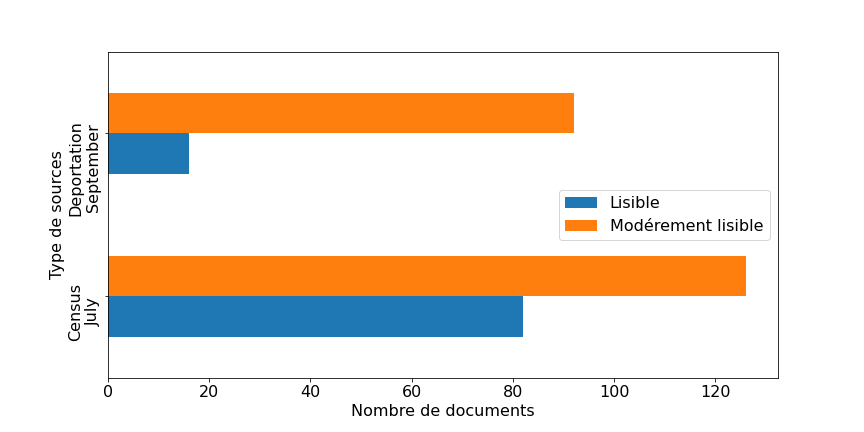
\includegraphics[width=\textwidth]{images/sources_legibility.png}
                    \vspace{-2em}
                    \caption{Analyse de la lisibilité des sources (voir \hyperref[analyse3]{le code}).}
                    \label{fig13}
                \end{figure}
                
                En dépit de ces difficultés, les données numérisées de l'\gls{ushmm} sont assez remarquablement fidèles aux archives. Elles conservent fautes et accentuations erronées des originaux et parviennent à restituer les informations peu lisibles qui font sens.
                
                \begin{figure}[!ht]
        			\centering
                    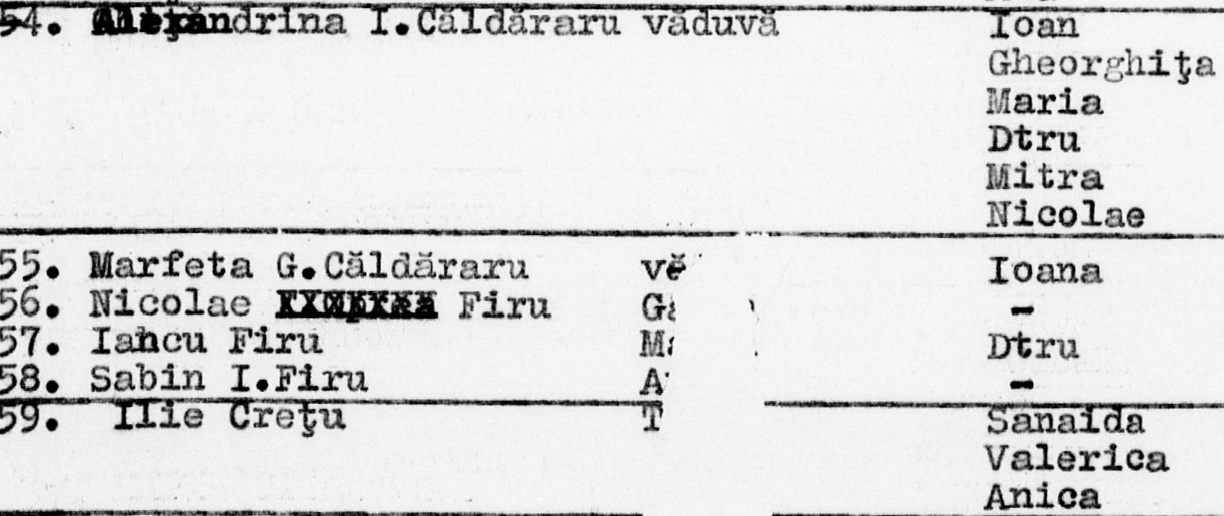
\includegraphics[width=13cm]{images/rg_25_050m_0009_00000784_detail.jpg}
                    \caption{Detail de liste\footcite[][Copyright \textit{Arhivele Naţionale ale României}]{rg-25.050mfileid:45869SelectedRecordsVarious}.}
                    \label{fig14}
                \end{figure}
                \vspace{-2em}
                \pagebreak
                
                \begin{savenotes} % Pour traiter les footnotes dans tabular (+ package footnotes)
                \begin{table}[ht]
                \centering
                \renewcommand\cellalign{cl}
                    \begin{tabular}{|c|c|c|c|}
                        \hline
                        Prénom & Nom & Statut Familial & Statut marital\\\hline
                        Alexandrina\footnote{Le prénom est restitué malgré les ratures.} I & Caldăraru & Self & Widowed\footnote{Veuve (\textit{văduvă}).}\\
                        Ioan & Căldăraru & Child & \\
                        Gheorghița & Căldăraru & Child &\\ 
                        Maria & Căldăraru & Child & \\
                        Dtru & Căldăraru & Child & \\
                        Mitra & Căldăraru & Child & \\
                        Nicolae & Căldăraru & Child & \\
                        Marfeta G & Căldăraru & Self & Married\\
                        Vă??\footnote{Les lacunes sont indiquées par les points d'interrogation.} & Căldăraru & Wife & Married\\
                        Ioana & Căldăraru & Child & \\
                        Nicolae\footnote{Les biffures ne sont pas prises en compte.} & Firu & Self & Married\\
                        G\footnote{Cette entrée devrait être \og{}G??\fg{}, mais cela relève du détail.} & Firu & Wife & Married\\
                        Iancu & Firu & Self & Married\\
                        Ma?? & Firu & Wife & Married\\
                        Dtru & Firu & Child & \\
                        Sabin I & Firu & Self & Married\\
                        A?? & Firu & Wife & \\
                        Ilie & Crețu & Self & Married\\
                        T?? & Crețu & Wife & Married\\
                        Sanaida & Crețu & Child & \\
                        Valerica & Crețu & Child & \\
                        Anica & Crețu & Child & \\\hline
                    \end{tabular}
                    \caption{Le tableau numérique correspondant à la figure \ref{fig14}\label{tab10}}
                \end{table}
                \end{savenotes}
                
                Les rares exceptions concernent en particulier les inscriptions qui chevauchent les lignes des tableaux, cette superposition ayant parfois pour effet de manquer un ou plusieurs noms de la case, ou un changement d'information (voir la note \ref{note1} du tableau \ref{tab5}).
                
                Le deuxième cas de figure observé concerne certains renseignements dactylographiés et biffés ou commentés de manière manuscrite. Dans l'exemple ci-dessous, ces personnes ont tout de même été incluses (deux fois puisqu'elles l'étaient également aux lignes 131 et 132 du document).
                
                \begin{figure}[!ht]
        			\centering
                    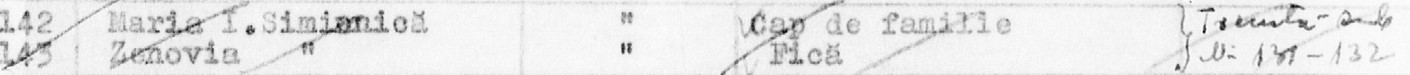
\includegraphics[width=15cm]{images/rg_25_050m_0009_00000560_detail.jpg}
                    \caption{Detail de liste\footcite[][Copyright \textit{Arhivele Naţionale ale României}]{rg-25.050mfileid:45835SelectedRecordsVarious}.}
                    \label{fig15}
                \end{figure}
                \vspace{-2em}
                
                \pagebreak
                
                Cette phase d'analyse permet de dégager les spécificités de notre corpus et d'entrevoir les premières actions de standardisation, de correction et d'enrichissement à mener. En ce sens, cette étape procure également des clés pour le choix des solutions qui devront être mises en œuvre pour réaliser les traitements. 
                
                
	    \section{Préparation des données}
	    
	        \subsection{Le choix des outils}
	        
	            \subsubsection{Les outils disponibles}
	    
        	        Malgré l'abondance de littérature sur le sujet, il apparaît que peu d'outils complets soient disponibles en accès libre (\textit{open access}).
        	        
        	        D'une part, les programmes mis au point pour les projets répondent largement aux besoins ponctuels et précis pour lesquels ils ont été conçus. Nous avons vu précédemment que les approches sont effectivement très dépendantes du type de données. Les auteurs détaillent parfois quelques-uns des algorithmes produits mais le plus souvent, le détail des opérations de traitement ne sont pas disponibles.
        	        
        	        D'autre part, un certain nombre de solutions sont développées par le secteur privé, qui peut également intervenir en appui des projets de recherche.
        	        
        	        Deux ressources proposent des listes de logiciels ou de modules en différents langages de programmation (principalement Python, R ou Java) \footcites{DatamatchingsoftwareListFree,ropeladderRecordLinkageResources2022}. Parmi eux, seulement cinq disposent d'une interface graphique (\textit{graphical user interface} ou GUI).
        	        
        	        Les solutions \textit{OpenRefine} et \textit{Dataiku} peuvent également être exploitées pour réaliser des couplage de données.
        	        
        	        Concernant les calculs de distance, une multiplicité de modules existent, parmi lesquels de très diverses implémentations des algorithmes formels des différentes distances.
	            
	            \subsubsection{Les besoins du projet et premier arbitrage}
	            
	                L'objectif du travail relatif à l'appariement est double~:
	               \vspace{0.8em} 
	               \begin{enumerate}
	                   \item d'une part, de créer des outils qui permettent de qualifier l'appariement déjà réalisé, le compléter et le corriger, voire de l'automatiser en partie\footnote{En particulier pour les futurs appariements.}~;
	                   \item d'autre part, que ces solutions soient réalisées de telle sorte que leurs composants puissent être réutilisés et adaptés à de futurs travaux.
	               \end{enumerate}
	               \vspace{0.8em}
	               Plus qu'un flux (semi-)automatisé d'appariement sur le corpus étudié lors de la phase courante du projet, il convient de mettre en place des modules qui puissent être recyclés, adaptés pour de futurs appariements, pour les phases ultérieures du projet ou sur d'autres projets.
	               
	               Ainsi la standardisation et le nettoyage des données (suppression des diacritiques, des ponctuations, passage en casse uniforme) constituent des étapes qui peuvent largement être réutilisées.
	               
	               La correction, l'enrichissement des variables, de même que l'indexation, les règles de blocage ou de classification, dépendront en revanche bien davantage de la disponibilité des données dans les autres sources qui viendraient à être étudiées dans le futur.
	               \newline
	               
	               Du point de vue du contexte du projet, les solutions développées doivent être intelligibles, aisément modifiables et en adéquation avec les compétences de l'équipe projet.
	               
	               En outre, la prise en main doit être relativement rapide afin de pouvoir fournir les différents livrables au prestataire en fonction des échéances planifiées~:
	               \vspace{0.8em}
	               \begin{itemize}
	                   \item 20 avril 2022~: livraison d'un premier fichier d'individus appariés regroupés par famille~;
	                   \item mai 2022~: évaluation de la congruence des appariements~;
	                   \item juin 2022~: modélisation des données~;
	                   \item juillet 2022~: détermination des itinéraires de trains et géolocalisation, correction des datasets~;
	                   \item 25 juillet 2022~: initialisation de la phase d'importation des données dans Geovistory\footnote{Voir la note \ref{geo}}~;
	                   \item fin août 2022~: chargement des données dans Geovistory\footnote{Voir la note \ref{geo}}, création des comptes.
	               \end{itemize}
	               \vspace{0.8em}
	               
	               Compte-tenu de ces contraintes, l'équipe effectue un premier arbitrage concernant le cadre de travail du projet.
	               
	           \subsubsection{Choix de l'environnement technique~: le langage Python}    
	               
	               En lien avec les ingénieurs de la plate-forme géomatique de l'\gls{ehess}, mais également eu égard aux programmes et langages utilisés par l'équipe mais également par le prestataire, l'arbitrage s'est porté sur un processus en Python\footnote{Langage de programmation interprété, voir \url{https://www.python.org/}}, qui dispose de l'ensemble des modules nécessaires au travail envisagé et garantira la pérennité et l'adaptabilité des solutions développées dans le cadre de la mission.
	               
	               Du point de vue de l'organisation, la plateforme géomatique de l'\gls{ehess} utilise \og{}Colaboratory\fg{}, ou \og{}Colab\fg{}\footnote{\og{}Colab\fg{} est un produit de Google Research qui permet d'écrire et d'exécuter un code Python dans un navigateur. Voir \url{https://research.google.com/colaboratory/faq.html?hl=fr}} pour collaborer sur des projets de programmation et le suivi de stage.
	               
	               Enfin, les données sont au format \acrshort{csv}. Les échanges avec le prestataire s'effectuent également dans ce format.
	               
	               Aussi, le traitement des fichiers sera réalisé avec~:
	               \vspace{0.8em}
	               \begin{itemize}
	                   \item Pandas\footnote{Voir \url{https://pandas.pydata.org/}}, une bibliothèque écrite pour le langage de programmation Python, en ce qui concerne la manipulation et l'analyse des données~;
	                   \item après évaluation, un choix parmi les bibliothèques, programmes ou modules dédiés au calcul des distances et aux appariements.
	               \end{itemize}
	               \vspace{0.8em}
	               
	               Les spécifications de la bibliothèque Pandas sont disponibles à \url{https://pandas.pydata.org/docs/}.
	               
	               Afin de pouvoir évaluer les solutions Python nécessaires à l'étude, la préparation des données constitue un préalable.
	                
	        \subsection{La standardisation des données}
	            
	            Il ressort de l'analyse des données que les actions suivantes seront nécessaires, que ce soit pour tester les outils, qualifier l'appariement ou évaluer son automatisation.
	            
	            Notons que ces étapes devraient être exécutées dans cet ordre~:
	                
	            \begin{enumerate}
	                \item assurer la correspondance des encodages et des formats des fichiers et de variables à comparer, afin de pouvoir traiter les chaînes de caractères dans le format adéquat et ainsi éviter des erreurs dans le fonctionnement des procédures~;
	                \item nettoyer les chaînes de caractères, à savoir~:
	                    \begin{enumerate}
	                        \item d'abord, supprimer les diacritiques pour non seulement optimiser les comparaisons futures, entre \og{}Căldăras\fg{} et \og{}Căldăra\textcolor{red}{ş}\fg{} par exemple, mais aussi pour réduire l'éventail de signes à traiter dans les expressions régulières ultérieures~;
	                        \item convertir en minuscule, pour les mêmes raisons~;
	                    \end{enumerate}
	                \item supprimer les ponctuations qui peuvent l'être à ce stade (voir ci-dessous)~;
	                \item corriger les entrées si possible (abréviations usuelles de prénoms)~;
	                \item segmenter les champs le cas échéant~;
	                \item enrichir les données le cas échéant (en particulier les genres).
	            \end{enumerate}
	        
	            \subsubsection{Encodage et formats}
	            \label{encod}
	                Cette opération est réalisée lors de la lecture et de la création des dataframe Pandas à partir des datasets (voir le code \ref{format_code}).
	                
	                Les fichiers du projet ont une structure bien définie (voir \ref{modele}), le fichier de l'\gls{ushmm} étant une source originale immuable et les fichiers en provenance du prestataire correspondant à un schéma défini, on s'assure de les charger selon les mêmes conventions, à savoir~:
	                
	                \begin{enumerate}
	                    \item au format UTF-8 (notamment du fait de l'accentuation de la langue)~;
	                    \item au format \acrshort{csv} délimité par \og{};\fg{}, par convention et pour éviter de possibles erreurs avec les virgules présentes dans de multiples champs\footnote{Certains fichiers originaux étaient corrompus de cette façon.}~;
	                    \item aucune colonne des fichiers n'est utilisée comme index du dataframe lors des chargements, une telle opération n'est effectuée que de manière réfléchie et volontaire à certains points du script~;
	                    \item toutes les données sont chargées au format texte (à défaut, Pandas tente de déterminer le type de données seul et le résultat peut varier sur un même type de données, en fonction des fichiers)~;
	                    \item une exception notable concerne les fichiers originaux de l'\gls{ushmm} pour lesquels les âges peuvent contenir du texte comme évoqué plus haut (voir \ref{age_desc}). Un convertisseur transforme ces entrées problématiques en chiffre (la fonction \textit{Convert\_Age(x)}).
	               \end{enumerate}
	            
	                En résumé, l'approche d'importation est assez stricte. L'expérience a montré que la bibliothèque Pandas ne parvient pas à fournir des résultats appropriés et constants lorsqu'elle est laissée autonome pour ces opérations.
	            
	                \label{stdcol}Enfin, après avoir chargé les fichiers, une conversion  des labels d'attributs est effectuée au moyen d'une table de conversion, afin d'assurer la concordance des variables\footnote{La table \textit{standard\_columns.xlsx}.} (voir la fonction \textit{Change\_Column\_Names(df, dict)} en annexe \ref{stdcol_code}).
	                
	            \subsubsection{Standardisation des chaînes}
	            \label{ascii}
	                
	                L'objectif, entre autres, est de neutraliser les différences de casse, les variations de diacritiques sans perte d'information (voir le code \ref{ascii_code}), au moyen du module \textit{unidecodedata}\footnote{Voir \url{https://docs.python.org/fr/3/library/unicodedata.html}.} et d'expressions régulières dans la fonction \textit{Normalise(df)}.
	                \pagebreak
	                
	                \paragraph{Les expressions régulières}\mbox{}\\
	                
	                Plutôt que de tenter de sélectionner les caractères à supprimer, les expressions régulières sont conçues pour ne sélectionner que les registres souhaités, à savoir l'alphabet latin non accentué obtenu après la normalisation effectuée à l'étape précédente.
	                
	                Sont aussi conservées les espaces naturellement, et quelques ponctuations.
	                
	                \paragraph{La question des signes de ponctuations}\mbox{}\\
	                
	                Les caractères \og{}-\fg{}, \og{}?\fg{} et \og{}.\fg{} ont été maintenus.
	                Le tiret d'abord car il intervient dans de nombreuses abréviations que le point suivant entend développer, une étape qui ne peut encore intervenir compte-tenu de l'état des chaînes à ce stade.
	                Avec le point d'interrogation aussi, puisqu'ils remplacent des lettres illisibles dans les originaux. Ce point n'est pas entièrement neutre car ils sont comptabilisés comme un caractère dans les mesures de distances et, selon les mesures, les scores ne sont pas équivalents\footnote{Neutre pour Levenshtein, -5\% à -20\% pour les autres distances, en fonction du signe et de sa position.}. Néanmoins, nous souhaitions conserver cette information à la lecture des résultats.

	                Concernant le caractère point \og{}.\fg{}, il ne peut être supprimé sans pré-traitement dans les chaînes du type \og{}N.C-tin\fg{}. Une espace doit être insérée afin de pouvoir segmenter \og{}N\fg{} et \og{}C-tin\fg{}.
	                L'approche doit être différente des situations suivantes~: \og{}N. C-tin Dimitru\fg{} (espace déjà présente), \og{}..rtina\fg{} ou \og{}Gheorgh...\fg{} (en lieu et place de caractères illisibles\footnote{Cas absent du recensement et de la déportation mais présent sur d'autres fichiers.}). Ce point est donc traité ultérieurement par la fonction \textit{Dot(df, var)}.
	            
	            \subsubsection{Développement des abréviations usuelles}
	            
	            
	               Un certain de noms et prénoms abrégés peuvent faire l'objet d'un développement d'abréviations, comme \og{}C-tin\fg{} en \og{}Constantin\fg{}.
	               
	               En revanche ce n'est pas toujours possible, lorsque de multiples orthographes et variantes par genre existent. Ainsi \og{}Gh\fg{} peut correspondre à \og{}Ghita\fg{}, \og{}Gheorgheta\fg{},\og{}Gheorghita\fg{}, \og{}Gheorghina\fg{}.
	               
	               \label{spell}La conversion est effectuée par la table \textit{spelling.xlsx} chargée et convertie en dictionnaire.
	               Cette opération ne fait pas l'objet d'une fonction de part sa simplicité (voir le code \ref{spell_code}).
	               
	           \subsubsection{Segmentation des prénoms et noms}
	            \label{segment}
	            
	               Afin de pouvoir analyser les éléments au niveau atomique, il est nécessaire de segmenter les informations pour les prénoms et noms qui comportent plusieurs mots ou groupes de mots.
	               
	               Il s'agit en particulier des surnoms, et des agrégations de noms, courantes dans le contexte historique et culturel (voir \ref{spec_noms}).
	               
	               À l'aide d'expressions régulières, les surnoms introduits par \textit{zis} ou \textit{zisa} (\og{}dit\fg{} et \og{}dite\fg{} respectivement) sont extraits et retirés des prénoms ou noms par la fonction \textit{Appellation(df, cols)} (voir le code \ref{segment_code}).
	               
	               Les prénoms et noms multiples sont segmentés par la fonction \textit{Split\_Names(df, cols)}.
	              
	            \subsubsection{Enrichissements}
	            \label{enrich}
	            
	               Après avoir standardisé les données, il est possible d'apporter plusieurs enrichissements afin de faciliter les comparaisons.
	               
	               \paragraph{Noms complets}\mbox{}\\
	               \label{fullnme}
	               
	               Disposer du nom complet pourrait être intéressant pour rechercher et valider les paires lorsque ces informations sont identiques entre fichiers. C'est le rôle de la fonction \textit{Fullname(df)} (voir le code \ref{fullnme_code}.

	               \paragraph{Années de naissance}\mbox{}\\
	               
	               \label{birth}L'analyse avait également révélé la disponibilité d'une quantité raisonnable d'âge des individus (variable dans le temps) mais de peu d'années de naissance.
	               
	               En fonction de l'année de production du document d'archive fournie par l'utilisateur, la conversion des âges en années de naissance est réalisée par la fonction \textit{Compute\_Birthyear(df, doc\_year: int, file)} (voir le code \ref{birth_code}).
	               
	               Ainsi, un âge de 42 ans sur un document de 1942 permet de renseigner une année de naissance de 1900.

	               \paragraph{Le genre}\mbox{}\\
	               \label{gender}
	               
	               Nous avions observé que le genre ne pouvait pas être déduit d'autres champs comme le statut familial ou marital (voir \ref{genre}).
	               
	               Néanmoins, des genres ont pu être inférés à partir des prénoms. La prévalence de ces derniers par genre a été analysée à partir de leur distribution dans un extrait normalisé de ces données, sur l'ensemble du corpus (plus de 130\,000 entrées).
	               
	               Une table \textit{gender.csv} est ainsi obtenue et exploitée par la fonction \textit{Derive\_Gender(df)} (voir le code \ref{gender_code}).
	               
	               Le gain est substantiel puisque cette opération permet de doubler le taux de couverture (voir le graphique ci-dessous). 
	               
	               \begin{figure}[!ht]
        			\centering
                    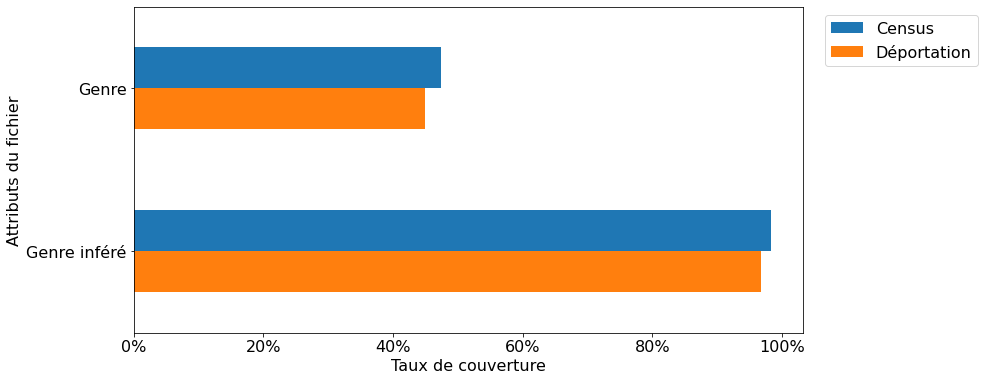
\includegraphics[width=\textwidth]{images/derived_gender.png}
                    \vspace{-2em}
                    \caption{Résultats de l'inférence des genres (voir \hyperref[analyse5]{le code}).}
                    \label{fig16}
                    \end{figure}
	                
	                En ce qui concerne la qualité de la donnée ainsi obtenue, la comparaison avec les données originales est positive et révèle un taux de correspondance important avec les informations des archives.
	                
	                Par exemple, sur les 7\,617 personnes de sexe féminin enregistrées dans les archives, le genre inféré est conforme pour 7\,419 d'entre elles.
	                
    	            \begin{table}[htbp]
    	            \centering
                    %\begin{adjustbox}{width=1\textwidth,center=\textwidth}
                    %\Large
                    %\settowidth\rotheadsize{}
                    \renewcommand\cellalign{cl}
                    %\renewcommand\arraystretch{2}
    			        \begin{tabular}{|c|c|c|}
    			        \hline
    			            \multicolumn{3}{|c|}{Census}\\\hline
    			            Genre & Genre inféré & Total \\\hline
    			            \multirow{3}{*}{female} & female & 7419 \\
                             & undetermined & 119 \\
                             & male & 79 \\\hline
                            \multirow{3}{*}{male} & male & 2510\\
                             & female & 77 \\
                             & undetermined & 23 \\\hline
                             \multirow{3}{*}{undetermined} & male & 7224\\
                             & female & 2632 \\
                             & undetermined & 1466 \\\hline
                        \end{tabular}
                        %\end{adjustbox}
                    \caption{Correspondance Genre et Genre inféré.}\label{tab11}
    			    \end{table}   
	                \vspace{-0.8em}
	                
	                La distribution homme - femme est en revanche inverse entre les deux données genre (majorité de femmes dans les sources mais davantage d'hommes inférés).
	                
	                Le sous-ensemble de 7\,224 nouveaux \og{}male\fg{} inférés est donc contrôlé. Les prénoms correspondent bien dans leur grande majorité à des prénoms indéniablement masculins.
	                \newline
	                
	                La préparation des données achevée, les tests d'appariements peuvent être initiés. Dans le cadre du projet, avant de passer à l'indexation et aux phases ultérieures, deux étapes intermédiaires étaient requises~: évaluer les outils de comparaison, puis les mettre à profit pour réaliser une première évaluation de la qualité du couplage manuel, afin que le prestataire puisse construire le prototype de la base de données.
	                \pagebreak

        \section{Analyse des outils de calcul de distance}
	        
	       \subsection{Les mesures de similarité}
	            \label{sim}
	        
	            Pour rappel, les publications suggèrent divers algorithmes pour évaluer le degré de correspondance de chaînes de caractères (voir la section \ref{similarite}). Elles disposent toutes d'avantages et d'inconvénients et s'adaptent diversement aux corpus sur lesquels elles sont mises en œuvre, en fonction des données.
	            
	            Aussi, nous avons dû réaliser des tests afin de comprendre quel(s) type(s) d'algorithme(s) utiliser sur nos recensements nominatifs.
	            
	            Comme de nombreuses implémentations ont été produites, notre choix s'est arrêté sur la librairie \textit{textdistance}\footnote{Voir~: \url{https://github.com/life4/textdistance} et \url{https://pypi.org/project/textdistance/}} car elle propose d'une part son propre ensemble de calculs de distance et elle prend également en charge les librairies les plus utilisées dans le domaine du \textit{fuzzy matching}.
	            
	            Différents calculs de distance ont été réalisés sur les données appariées manuellement, avec pour double objectif~:
	            
	            \begin{itemize}
	                \item analyser le comportement des différents algorithmes sur les données du projet et évaluer lesquels seraient les plus appropriés pour notre étude~;
	                \item obtenir une première vue d'ensemble de l'appariement manuel.
	            \end{itemize}
	            
	            Conformément aux attentes, les différents scores témoignent de particularités différentes. Après analyse, une combinaison de mesures nous apparaît être la plus appropriée au regard de notre premier objectif (qualification de l'appariement manuel).
	            
	            En effet, avec un Monge-Elkan sur le nom complet supérieur ou égal à 0.8, nous qualifions 3\,728 des 4\,391 paires, soit 86\%.
	            
	            Parmi ces paires~:
	            \begin{itemize}
	                \item 1\,993 sont des \textit{matchs} exacts (Levenhstein) sur à la fois le prénom et le nom~;
	                \item 370 \textit{matchs} exacts sur les prénoms et moins de un caractère d'écart sur le nom~;
	                \item 310 \textit{matchs} partiels sur les prénoms et plus de un caractère différent sur le nom, validés après examen~;
	                \item 108 correspondances parfaites après sélection du meilleur prénom parmi les différents prénoms enregistrés~;
	                \item 134 inversions noms - prénoms~;
	                \item 322 pour lesquels moins de un caractère d'écart existe sur le nom, validés après examen~;
	                \item 290 validés avec un score de Jaro-Winkler supérieur à 80\%~;
	            \end{itemize}
	            ce qui résulte en 201 paires, dont l'orthographe est très affectée mais les personnes correspondent pour moitié, le delta regroupant des cas discutables.
	            \pagebreak
	            
	            Parmi les 663 paires appariées dont le score Monge-Elkan reste inférieur à 0.8, 395 obtiennent un score Levenshtein de 0.8 et plus sur la meilleure association de prénoms. Il s'agit pour la plupart de paires valides, pour lesquels on observe deux cas de figure principaux.
	            
	            D'une part, l'algorithme Monge-Elkan est négativement impacté par la présence d'une initiale supplémentaire en fin de nom complet. D'autre part, pour nombre de ces familles, un nom alternatif a été enregistré (les prénoms correspondent sur l'ensemble et seul le nom varie). Cela pourrait correspondre notamment à la sélection du nom du père dans un recensement et celui d'enfance de la mère pour la seconde liste.
	            
    	        Les 257 dernières personnes rapprochées sont vraisemblablement des erreurs pour la plupart, car peu de données correspondent, y compris les dates de naissance.
    	        Dans ce groupe, on observe également des individus qui, s'ils sont appariés correctement au niveau de la famille, les personnes ont été interverties entre elles.
    	        
    	        En conclusion, le nombre d'appariements corrects d'environ 86\% correspond aux attentes de l'équipe et satisfaisant, au regard des taux généralement obtenus sur ce type de données.
    	        
    	        Sur cette base, des indicateurs sont produits sur les paires, pour l'équipe comme pour le prestataire~:
    	        
    	        \begin{itemize}
	                \item un score de Levenshtein sur le nom complet~;
	                \item un score de Monge-Elkan sur le nom complet~;
	                \item un dénombrement des individus de même nom dans la zone géographique pour chacun des fichiers (comptage des homonymes potentiels)~;
	            \end{itemize}
	            \vspace{0.8em}
	            afin de disposer à l'avenir d'un indice de confiance sur les paires, comme pour réaliser les examens et corrections manuelles qu'il conviendrait d'apporter à l'appariement à une phase ultérieure.
	            
        \section{Essai d'un processus de couplage}
            \label{rl}
            
            Pour évaluer si d'autres individus auraient dû être liés en revanche, un nouvel appariement est nécessaire\footnote{Voir le code \ref{rl_code}}.
            Pour cette opération, initiée en fin de stage, le choix de la solution s'est porté sur la bibliothèque \textit{Record Linkage}\footcite[][Voir également~: \url{https://github.com/J535D165/recordlinkage} et \url{https://pypi.org/project/recordlinkage/}]{debruinPythonRecordLinkage2019}, dédiée au couplage et à la  déduplication d'enregistrements dans ou entre des sources de données, pour lesquels elle fournit la plupart des outils nécessaires.
            \pagebreak
	            
	       \subsection{Indexation et blocage}
	            
                \textit{Record Linkage} permet d'indexer les sources, dans leur totalité, ou en pré-définissant des clés de blocage (voir la section \ref{blocking}).
                
                Concernant le recensement de juillet et de la déportation, les fichiers comportent respectivement 21\,549 et 13\,033 enregistrements, soit 280\,848\,117 comparaisons à réaliser sans clé de blocage.
                
                Par conséquent, la définition de telles clés s'impose. Sur ce sujet, un très grand nombre de possibilités existent puisqu'il est possible d'utiliser un attribut seul pour servir de clé, mais également toute combinaison d'attributs ou subdivision d'attributs. Sans faire une liste exhaustive, les clés de blocage usuelles sont~:
                
                \begin{enumerate}
                    \item le genre (les individus de même sexe seulement sont comparés)~;
                    \item les éléments d'adresses, en particulier ceux qui sont standardisés comme le code postal, des noms de villes normalisés~;
                    \item des années de naissance~;
                    \item de manière générale, tout élément qui permet de distinguer des groupes plus restreints à comparer sur la base d'éléments invariants~;
                    \item des unions de tout ou partie de ces éléments.
                \end{enumerate}
                
                Dans le contexte du projet, une clé de blocage en particulier nous a intéressé. Il s'agit du code des localités mis en place pour le projet. Comme nous l'avons rappelé, les deux recensements sont proches et peu de changements, dans les familles ou adresses, sont attendus entre ces deux événements.
                
                L'ajout de cette clé de blocage permet de restreindre le nombre de comparaisons à 4\,861\,124~: seuls les individus enregistrés dans la même localité seront comparés les uns aux autres.
                
                
                Une clé de blocage sur à la fois le code localité et le genre réduit l'index des paires à 2\,528\,167.
                \newline
                
                Sur cette dernière base, nous définissons les règles de comparaison des enregistrements.
                
            \subsection{Comparaison des paires et classification}
	            
	            Pour rappel (voir la section \ref{compare}), cette étape permet de choisir les attributs (valeurs) qui seront rapprochés et testés selon les critères choisis, par exemple une similarité supérieure à 0.7 (soit de 70\%).
	            
	            Les premiers tests effectués avec un nombre limité de règles ont montré qu'il est alors relativement difficile de catégoriser les paires liées de celles non liées.
	            \pagebreak
	            
	            En effet, avec une comparaison sur les seuls prénoms, noms et date de naissance par exemple, pour toutes les paires sans cette dernière information, le résultat consiste en une liste de \textit{matchs} potentiels dont les noms et prénoms ont tous atteint les seuils de similarité. Il est alors peu aisé de distinguer les paires les plus probantes~:

	            \begin{table}[htbp]
    	            \centering
                    %\begin{adjustbox}{width=1\textwidth,center=\textwidth}
                    %\Large
                    %\settowidth\rotheadsize{}
                    \renewcommand\cellalign{cl}
                    %\renewcommand\arraystretch{2}
    			        \begin{tabular}{|c|c|c|c|c|c|}
    			        \hline
			            \multicolumn{2}{|c|}{Index}&\multicolumn{2}{|c|}{Fichier 1}&\multicolumn{2}{|c|}{Fichier 2}\\\hline
			            \Centerstack{ID\\Fichier 1} & \Centerstack{ID\\Fichier 2} & Nom & \Centerstack{Année\\naissance} & Nom & \Centerstack{Année\\naissance} \\\hline
                        8750260 & 8799761 & bozsodi susana & 1934 & dondos susana &  \\
                        8750282 & 8799761 & dondos elisabeta & 1929 & dondos susana &  \\
                        8750283 & 8799761 & dondos ghizela & 1930 & dondos susana &  \\
                        8750282 & \cellcolor{red}8799762 & dondos elisabeta & 1929 & dondos iuliu &  \\
                        8750283 & \cellcolor{red}8799762 & dondos ghizela & 1930 & dondos iuliu &  \\
                        8750291 & \cellcolor{red}8799762 & dondoczi semoil & 1923 & dondos iuliu &  \\
                        8750361 & \cellcolor{red}8799762 & dondoczi vasile & 1924 & dondos iuliu &  \\
                        8750251 & 8799789 & dondos iuliu & 1934 & dondos rozalia &  \\
                        8750291 & 8799789 & dondoczi semoil & 1923 & dondos rozalia &  \\
                        8750361 & 8799789 & dondoczi vasile & 1924 & dondos rozalia &  \\
                        8750251 & 8799790 & dondos iuliu & 1934 & dondos paraschiva &  \\
                        8750361 & 8799790 & dondoczi vasile & 1924 & dondos paraschiva &  \\
                        8750251 & 8799792 & dondos iuliu & 1934 & dondos elisabeta &  \\
                        8750361 & 8799792 & dondoczi vasile & 1924 & dondos elisabeta &  \\
                        8750251 & 8799793 & dondos iuliu & 1934 & dondos ghizala &  \\
                        8750291 & 8799793 & dondoczi semoil & 1923 & dondos ghizala &  \\
                        8750361 & 8799793 & dondoczi vasile & 1924 & dondos ghizala &  \\
                        8750251 & 8799794 & dondos iuliu & 1934 & dondos rozalia &  \\
                        8750282 & 8799794 & dondos elisabeta & 1929 & dondos rozalia &  \\
                        8750283 & 8799794 & dondos ghizela & 1930 & dondos rozalia &  \\
                        8750291 & 8799794 & dondoczi semoil & 1923 & dondos rozalia &  \\
                        8750361 & 8799794 & dondoczi vasile & 1924 & dondos rozalia &  \\
                        8750251 & 8799796 & dondos iuliu & 1934 & dondos ileana &  \\
                        8750283 & 8799796 & dondos ghizela & 1930 & dondos ileana &  \\
                        8750291 & 8799796 & dondoczi semoil & 1923 & dondos ileana &  \\
                        8750315 & 8799796 & fodor ileana & 1936 & dondos ileana &  \\
                        8750361 & 8799796 & dondoczi vasile & 1924 & dondos ileana &  \\\hline
                    \end{tabular}
                    %\end{adjustbox}
                \caption{Exemple simplifié de résultats de comparaison.}\label{tab12}
			    \end{table}   
                \vspace{-0.8em}
            
	            Un seul individu du fichier 2 (surligné en rouge) est rapproché avec plusieurs individus du fichier 1, autant de fois que les similarités définies sont respectées. Sans plus de critères, il est peu commode d'identifier les meilleures paires.
	            
	            Notons que le résultat ci-dessus est obtenu sur la base de seuils de similarité Jaro-Winkler de 0.7 (prénom) et 0.8 (nom), ce qui semble trop flou et permissif.
                \pagebreak
                
	            Afin d'obtenir davantage de critères discriminants, les règles suivantes peuvent être définies comme ci-dessous (parmi les premiers tests effectués)~:
	            
	            \begin{itemize}
	            \vspace{0.8em}
	                \item prénom 1~: similarité de Levenshtein >= 0.7~;
	                \item prénom 2~: similarité de Levenshtein >= 0.7~;
	                \item nom~: similarité de Levenshtein >= 0.8~;
	                \item nom complet~: similarité de Levenshtein >= 0.8~;
	                \item année de naissance~: comparaison exacte\footnote{Il est en possible de tester les valeurs numériques avec une tolérance, mais cette option engendrait un dépassement des capacités de mémoire.}~;
	                \item identifiant famille~: comparaison exacte\footnote{Ceci n'est possible que sur la réconciliation d'un corpus préalablement apparié, ce qui était le cas dans cet essai.}~;
	                \item genre inféré~: comparaison exacte\footnote{Le genre étant une clé de blocage, les valeurs correspondent, néanmoins on peut ici clarifier que des valeurs manquantes ne constituent pas un résultat positif.}~;
	                \item statut familial~: comparaison exacte~;
	                \item identifiant localité~: comparaison exacte\footnote{Idem.}.
	            \end{itemize}
	            \vspace{0.8em}
	            Les paramètres ci-dessus procurent les performances suivantes~:
	            
	            \begin{table}[htbp]
    	            \centering
                    %\begin{adjustbox}{width=1\textwidth,center=\textwidth}
                    %\Large
                    %\settowidth\rotheadsize{}
                    \renewcommand\cellalign{cl}
                    %\renewcommand\arraystretch{2}
    			        \begin{tabular}{|c|c|}
    			        \hline
			            Mesure & Résultat\\\hline
			            Paires indéxées & 2\,092\,398\\\hline
			            Précision & 0,056\\\hline
			            Rappel & 0,809\\\hline
			            F1-Score & 0.105\\\hline
			            Durée & 5 minutes\\\hline
                    \end{tabular}
                    %\end{adjustbox}
                \caption{Résultats d'un test déterministe (règles à base de seuils).}\label{tab13}
			    \end{table}   
                \vspace{-0.8em}
                
                Le couplage produit 6\,227 paires potentielles (dont des propositions multiples pour un individu comme illustré dans la table \ref{tab12} ci-dessus).
                
	            Parmi elles, 3\,426 sont également liées dans l'appariement manuel et 2\,524 offrent le même couplage. Notons que la vaste majorité (2\,466) de ces paires communes recoupent les 86\% de paires jugées satisfaisantes dans l'analyse du couplage manuel.
	            \newline
	            
	            Pour restreindre encore le nombre de paires comparées et limiter la recherche aux enregistrements voisins, il est notamment possible d'utiliser la méthode des plus proches voisins (\textit{Sorted Neighbourhood}).
	            Le test est réalisé en mode d'apprentissage automatique non supervisé.
	            
	            L'indexation est paramétrée en \textit{Sorted Neighbourhood} sur le nom de famille, avec des clés de blocage sur le code localité et le genre inféré.
	            
	            Le nombre de paires candidates est drastiquement ramené à 53\,988 couples à classer.
	            \pagebreak
	            
	            Les résultats de cet appariement ont été les suivants~:
	            
	            \begin{table}[htbp]
    	            \centering
                    %\begin{adjustbox}{width=1\textwidth,center=\textwidth}
                    %\Large
                    %\settowidth\rotheadsize{}
                    \renewcommand\cellalign{cl}
                    %\renewcommand\arraystretch{2}
    			        \begin{tabular}{|c|c|}
    			        \hline
			            Mesure & Résultat\\\hline
			            Paires indéxées & 53\,988\\\hline
			            Précision & 0,346\\\hline
			            Rappel & 0,960\\\hline
			            F1-Score & 0.509\\\hline
			            Durée & 1-2 minutes\\\hline
                    \end{tabular}
                    %\end{adjustbox}
                \caption{Résultats d'un test \textit{Sorted Neighbourhood}.}\label{tab14}
			    \end{table}   
                \vspace{-0.8em}
	            
                Cet appariement produit 5\,692 paires potentielles (dont des propositions multiples pour un individu).
                
                Parmi elles, 3\,162 sont également liées dans l'appariement manuel et 2\,348 offrent le même couplage, avec 2\,295 de ces paires communes situées dans la tranche des 86\% de paires jugées satisfaisantes dans l'analyse du couplage manuel.
                
                Ces résultats sont intéressants dans la mesure où ils permettent de mesurer la performance de ce modèle sans entraînement préalable et donc d'évaluer son comportement sur des données nouvelles.
                \bigskip
                
                Sur ces paires, le nombre de correspondances entre les neuf attributs comparés est détaillé dans le tableau ci-dessous~:
                
                \begin{savenotes} % Pour traiter les footnotes dans tabular (+ package footnotes)
                \begin{table}[htbp]
    	            \centering
                    %\begin{adjustbox}{width=1\textwidth,center=\textwidth}
                    %\Large
                    %\settowidth\rotheadsize{}
                    \renewcommand\cellalign{cl}
                    %\renewcommand\arraystretch{2}
    			        \begin{tabular}{|c|c|c|c|}
    			        \hline
			            Correspondances&\Centerstack{Appariement\\manuel}&\Centerstack{Modèle\\(paires potentielles)}&\Centerstack{Modèle\\(paire uniques\footnote{La mesure est donnée à titre indicatif uniquement et effectuée sur les enregistrements pour lesquels une seule paire est proposée~: pour ceux proposés dans de multiples combinaisons, les résultats ne sont pas connus avant d'avoir arrêté un choix de paire, le cas échéant.})}\\\hline
                        9&21&23&16\\
                        8&425&533&423\\
                        7&1384&1789&1348\\
                        6&1011&1448&742\\
                        5&782&1669&266\\
                        4&495&230&38\\
                        1-2-3&273&-&-\\\hline
                        Total&4391&5692&2833\\\hline
                    \end{tabular}
                    %\end{adjustbox}
                \caption{Concordance des attributs par appariement.}\label{tab15}
			    \end{table}   
                \end{savenotes}
                
                Ces résultats donnent une idée du taux de confiance qui peut être accordé aux différentes paires. En effet, plus le nombre d'attributs correspondants est élevé, plus les deux enregistrements sont proches et donc susceptibles de référer à la même personne.
                \pagebreak                

                En résumé, il nous a été possible d'estimer la qualité de l'appariement réalisé manuellement et l'équipe l'a jugé satisfaisante à ce stade de la recherche. Le couplage peut encore être affiné, notamment par des corrections continues toujours en cours mais aussi par l'apport des informations additionnelles qui seront obtenues des rapprochements futurs avec les autres sources disponibles, en provenance des camps d'une part et d'autres recensements d'autre part.
                \smallskip
                
                Nous avons pu également tester des solutions de couplage programmées en Python avec \textit{Record Linkage}, dont certains résultats semblent insuffisants, d'autres prometteurs. Cette partie du travail reflète bien la difficulté de l'exercice du couplage de données relayée par la littérature. Nous discutons des perspectives d'amélioration et présentons le résultat matériel et concret du projet dans le prochain chapitre.
                
    \pagestyle{empty}
	\cleardoublepage
	\pagestyle{plain}			
	
	\chapter{Perspectives et réalisations concrètes}            
        \label{chap3}
        
        \section{Perspectives d'amélioration}
            
            \subsection{Fouille et segmentation}
            
                Nous avons vu que les sources sont parfois pauvres en informations et que la graphie des noms est extrêmement variable.
                
                Une fouille et une segmentation plus poussées permettraient de réduire les informations parasites et faire mieux ressortir celles qui sont pertinentes, un travail entamé mais qui nécessite d'être poursuivi~:
                
                \begin{itemize}
                    \item extraire les prénoms des chefs de famille~;
                    \item isoler et éliminer les initiales correspondantes imbriquées dans les prénoms~;
                    \item identifier les initiales communes à plusieurs membres d'une famille afin de les traiter séparément, même en l'absence du prénom du père~;
                    \item dresser les listes des patronymes (pour comparer les noms alternatifs possibles) et prénoms au niveau des familles~;
                    \item convertir les âges en tranches d'âges pour autoriser une comparaison floue~;
                    \item enrichir le statut familial en fonction de l'âge (par exemple attribuer la valeur \og{}Child\fg{} aux personnes de moins de 16 ou 17 ans, là où l'information est actuellement manquante)~;
                    \item poursuivre la normalisation des fautes orthographiques sur les prénoms~;
                    \item évaluer la pertinence de subdiviser la table de correction orthographique par genre, afin d'introduire davantage de développements d'abréviations~;
                    \item considérer le développement ou la normalisation des \og{}i\fg{} en \og{}ioan\fg{} des \og{}g\fg{}, \og{}gh\fg{} et \og{}ghe\fg{} en \og{}gheorghe\fg{} ou \og{}gheorghita\fg{}, les deux formes les plus courantes~;
                    \item compléter la table d'attribution des genres pour les prénoms pour lesquels l'analyse n'a pas identifié de résultats probants.
                \end{itemize}
                
                Cette liste de pistes non exhaustive reflète bien l'ampleur des possibilités, à mettre en perspective avec les attentes du projet et les ressources disponibles pour effectuer ces développements.
                
            \subsection{Optimiser les modèles}
            
                \subsubsection{Renforcer l'indexation}
                
                    De la même façon, le modèle en lui même peut largement gagner en efficacité. Développé en fin de stage, il n'a pas pu bénéficier du nombre de tests et d'ajustements nécessaires à de meilleures performances.
                    
                    Concernant l'indexation d'abord, les possibilités sont aussi diverses qu'en matière de fouille et de segmentation. La création de nouvelles clés de blocage plus ou moins strictes selon les informations à apparier est par exemple envisageable.
                    
                    Les informations des listes des camps notamment sont extrêmement limitées. Pour celles-ci, l'introduction de clés de blocage sur une ou plusieurs des initiales pourrait réduire le nombre de faux positifs.
                    
                    Pour faire un parallèle avec la question des attributs discutée plus haut, les nouvelles données extraites des enregistrements peuvent constituer autant de clés efficaces, à l'instar des tranches d'âge.
                    
                    Bénéficier de davantage de \textit{blocking keys} peut autoriser des seuils de comparaison plus modérés ou une augmentation de la fenêtre de recherche dans l'approche des voisins triés.  
                
                \subsubsection{Diversifier les comparaisons}
                
                    La problématique est la même pour la comparaison. Avec neuf attributs actuellement, les possibilités sont limitées. Introduire de nouvelles entrées discriminantes à analyser fournirait autant d'indices supplémentaires dans le choix des vrais positifs.
                    
                    Deux autres leviers peuvent être mis en œuvre pour aider à la classification. En premier lieu, lors de l'agrégation des points de concordances (voir le tableau \ref{tab15}), une pondération différenciée peut être utilisée~: une même année de naissance est plus significative que la correspondance d'une tranche d'âge, elle même plus révélatrice qu'une ressemblance d'un deuxième prénom.
                    
                    Ensuite, une approche en plusieurs passages, progressivement plus permissifs, contribuerait à simplifier l'analyse des résultats en dégageant en priorité les paires fortement liées vers les cas moins éloquents.
                
                \subsubsection{Perfectionner les modèles}
                
                    Enfin, à propos des modèle en eux-mêmes, la conception de règles additionnelles et sur mesure renforcerait leur efficacité.
                    
                    À titre d'exemple, une comparaison croisée et systématique des prénoms et initiales pourrait être bénéfique.
                    
                    En outre, la mesure de distance utilisée pour estimer les similarités de l'appariement manuel n'est pas disponible dans la bibliothèque \textit{Record Linkage}. Le processus accepte cependant l'intégration de fonctions personnalisées, un biais par lequel la mesure de Monge-Elkan pourrait être implémentée. 
                    
                    D'autres modèles sont également à disposition  dans la bibliothèque \textit{Record Linkage} comme la régression logistique, les \textit{SVM}, autant d'alternatives possibles qui reflètent bien l'une des problématiques discutées dans la littérature, à savoir la difficulté de trouver la méthode la plus adaptée parmi l'offre très diversifiée d'algorithmes.
                
                \subsubsection{Développement du code Python}
                
                    Le code conçu au cours du projet comporte des limites à prendre en compte.
                    
                    Premièrement, il a été produit pour répondre à un besoin particulier en fonction des diverses échéances du projet. En conséquence, il n'a pas été développé comme un outil générique. Aussi, il ne peut en l'état s'adapter à différents corpus ou fonctionner sur des données non conformes. Il est basé sur la structure des données de l'\gls{ushmm}. Les labels de fichiers, d'attributs, le format de données sont intimement liés au schéma des sources \acrshort{csv} et des modèles mis en place avec le prestataire.
                    
                    Ensuite, il n'est pas construit comme une chaîne de traitement à proprement parler. S'il assure les différentes transformations les unes après les autres, il ne s'agit pas d'une application qui permettrait de sélectionner des fichiers en entrée pour disposer d'un dépôt de résultats au format \acrshort{csv} (ou autres), d'une interface de consultation, d'indicateurs. Il s'agit d'un programme en code, d'aide à la décision. Une des améliorations les plus immédiates serait d'ajouter des variables à certaines fonctions, notamment celle exploitant \textit{Record Linkage}, dans la mesure du possible, puisque la quantité d'options devrait être soigneusement choisie au regard du nombre important de possibilités de paramétrage.
                    
                    L'ajout d'une interface est techniquement réalisable avec \textit{Record Linkage} (RecordLinkage Annotator\footnote{Voir~: \url{https://github.com/J535D165/recordlinkage-annotator}}). Cependant, comme la plupart des systèmes d'annotation ou de validation\footnote{Notamment ceux utilisés pour les entraînements.} ne présentent pas les enregistrements \textit{dans leur contexte}, il est malaisé de classer des paires dans ces conditions. Sans afficher les données voisines permettant de lier ou non des paires, il faut souvent retourner à la source. Dans le contexte du projet, un examen des numérisations s'est révélé bien souvent nécessaire.

		\section{Les résultats concrets pour le projet}
		
			\subsection{Structurer et modéliser les données}
			
			    Dans le cadre d'un projet ambitieux comme \textit{La déportation des Roms en Transnistrie, 1942 - 1944. Trajectoires individuelles et destin collectif}, qui doit permettre des études statistiques et l'analyse des statuts administratifs,  des variables sociodémographiques et des parcours dans la dimension spatiale, la question de la définition des données, de leur modélisation est une étape indispensable.
			
			    \subsubsection{Le modèle de données}
			    \label{modele}
			        Afin de pouvoir exploiter massivement les documents identifiés, un modèle de données a été conceptualisé par l'équipe de recherche.
			        
			        \begin{figure}[!ht]
            			\centering
                        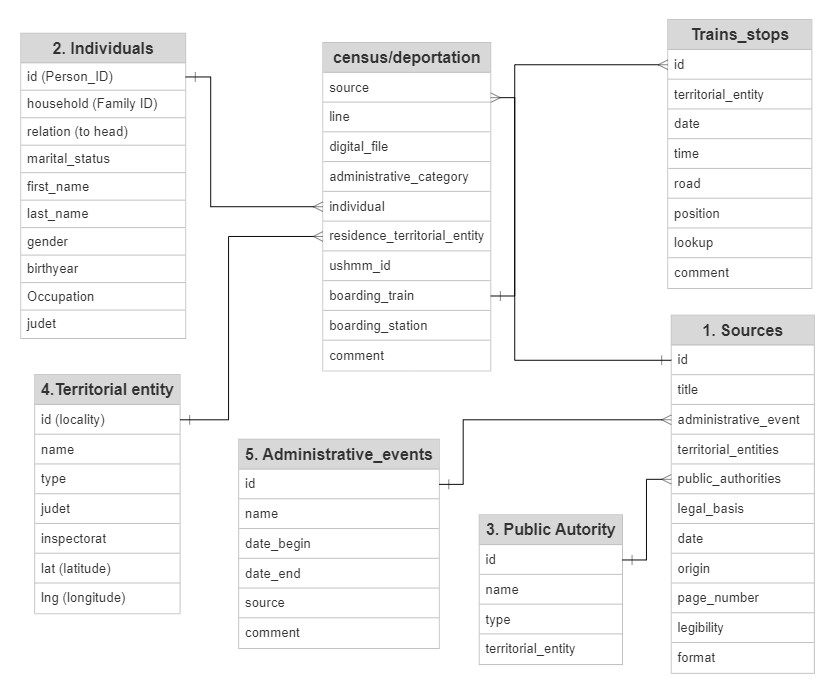
\includegraphics[width=\textwidth]{images/datamodel.jpg}
                        \vspace{-2em}
                        \caption{Modèle entités - associations.}
                        \label{fig17}
                    \end{figure}
                    \pagebreak
                    
                     En reprenant les informations de la documentation afin qu'elle puisse être exploitée, l’architecture de ces données met en relation cinq entités principales dans le modèle ontologique suivant~:
			        
			        \begin{enumerate}
			            \item les documents nominatifs~;
			            \item les individus~;
			            \item les autorités publiques~;
			            \item les entités territoriales~;
			            \item les évènements administratifs.
			        \end{enumerate}
                    
                    Le projet a été l'occasion de clarifier les définitions, les types de données afin que le prestataire puisse modéliser, renseigner les ontologies et intégrer les données dans son environnement.

				\subsubsection{Premières analyses de faisabilité}
				\label{parcours}
				    Un point clé du projet étant de permettre de reconstituer les parcours individuels et collectifs, une géolocalisation et une analyse temporelle des trains de déportation peut être réalisée, grâce aux sources mentionnant les horaires de départ, de point de passage et d'arrivée dans les diverses gares.
				    
				    L'organisation de la déportation est intimement liée à l'organisation territoriale de la Roumanie de 1942. C'est un point particulier que le projet entend étudier en détail.
				    
				    Ainsi, grâce aux données collectées, géocodées, le prestataire a pu procéder à des premières analyses qui laissent entrevoir un potentiel important pour la suite~:
				    
				    \begin{figure}[!ht]
            			\centering
                        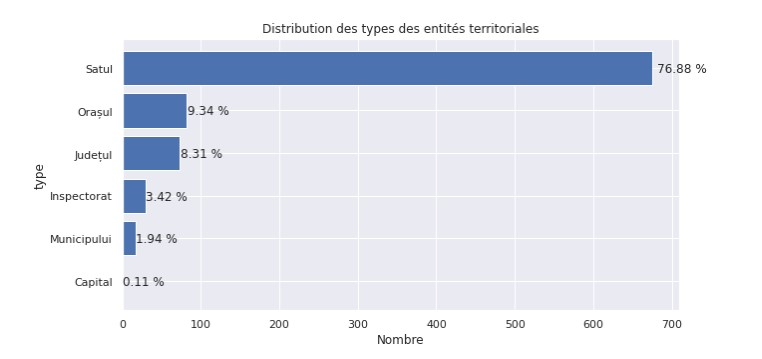
\includegraphics[width=16cm]{images/entites_terr_distrib.jpg}
                        \vspace{-1cm}
                        \caption[Types d'entités territoriales.]{Types d'entités territoriales\footnote{Préparé par Gaétan Muck, KleioLab GmbH.}.}
                        \label{fig18}
                    \end{figure}
                    \pagebreak
                    
                    \begin{figure}[!ht]
            			\centering
                        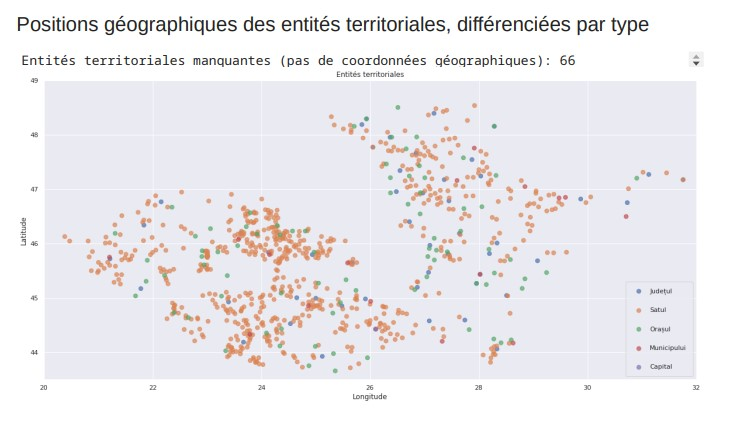
\includegraphics[width=\textwidth]{images/entites_terr_map.jpg}
                        \vspace{-1cm}
                        \caption[Carte des entités territoriales.]{Cartes des entités territoriales\footnote{Préparé par Gaétan Muck, KleioLab GmbH.}.}
                        \label{fig19}
                    \end{figure}
                    
                    \begin{figure}[!ht]
            			\centering
                        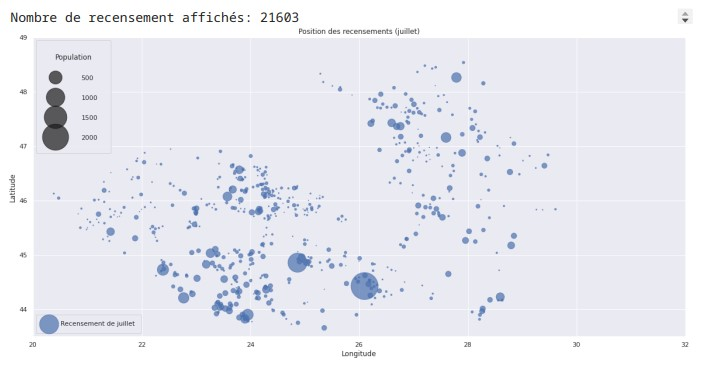
\includegraphics[width=15cm]{images/recensement_map.jpg}
                        \vspace{-1cm}
                        \caption[Les recensements en population.]{Les recensements de juillet 1942 en population\footnote{Id.}.}
                        \label{fig20}
                    \end{figure}
				    \pagebreak
				    
				    \begin{figure}[!ht]
            			\centering
                        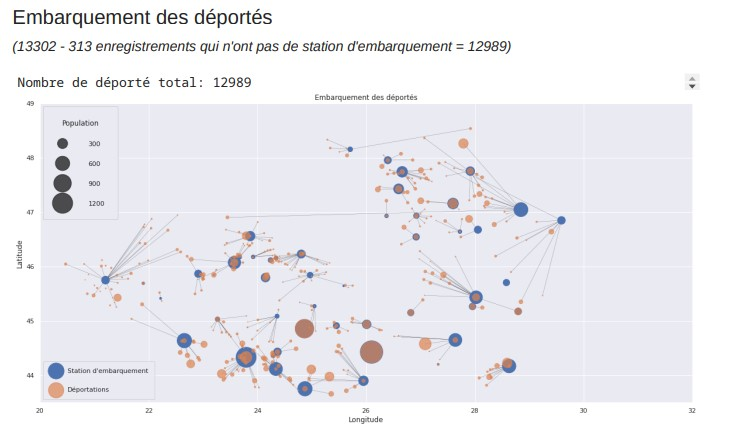
\includegraphics[width=15cm]{images/deportation_map.jpg}
                        \vspace{-0.8cm}
                        \caption[Carte de la déportation.]{Carte de la déportation\footnote{Préparé par Gaétan Muck, KleioLab GmbH.}.}
                        \label{fig21}
                    \end{figure}

				    \begin{figure}[!ht]
            			\centering
                        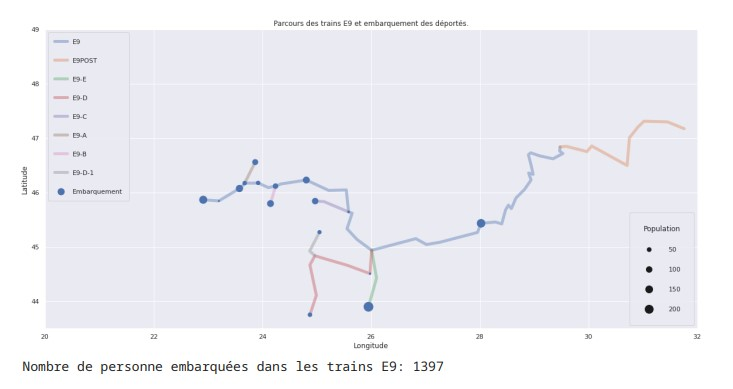
\includegraphics[width=\textwidth]{images/trains.jpg}
                        \vspace{-1.2cm}
                        \caption[Trajet d'un train.]{Trajet d'un train et ses effectifs dynamiques\footnote{Id.}.}
                        \label{fig22}
                    \end{figure}
                    
                    En élargissant la chronologie, depuis les lieux d'origine jusqu'au retour des personnes, une visualisation des parcours permet une analyse à différentes échelles. Au niveau d’une personne ou des membres d’une famille, de personnes originaires du même lieu, l'étude pourra faire ressortir des faisceaux de parcours, des trajectoires typiques ou, au contraire, mettre en lumière des cas limites intéressants.
				    \pagebreak


	\pagestyle{empty}
	\cleardoublepage
	\pagestyle{plain}			
		
		
	\chapter*{Conclusion}
		\addcontentsline{toc}{chapter}{Conclusion}% Ajout à la table des matières sans numérotation
		
		L'étude de la déportation des Roms est un projet multiscalaire portant sur un vaste corpus (125 000 entrées individuelles pour environ 1 500 documents). L'historiographie, récente mais riche, de cet événement est surtout centrée sur l'appareil d'État. Orienté autour des parcours des individus à différentes échelles, le projet se donne pour ambition de suivre effectivement les personnes, de faire une histoire totale, à la fois fine et globale, communauté par communauté, localité par localité.
		
		Un des points délicats d'une telle étude, qui détermine la qualité de l’ensemble de l’enquête est la duplication des identités entre les documents. Aussi, il faut établir une table de liens entre les personnes enregistrées dans les différentes archives administratives, en s'appuyant sur les noms, prénoms et en évaluant au regard des autres informations comme l’âge, les noms des membres de la famille ou encore le lieu de résidence s’il s’agit des mêmes personnes.
		
		Cette entreprise d'appariement est rendue délicate par la nature de l'information elle-même. En effet, les données nominatives sont souvent très variables et le sont encore davantage sur les documents historiques. Les agents en charge de constituer les listes, les personnes elles-mêmes ne sont pas toujours constantes dans la manière de s'identifier ou de préciser un âge, surtout dans des territoires où l'état civil n'est pas encore fortement établi.
		
		Aussi, l'étude s'est confrontée à des données relativement inégales, imprécises mais surtout dénaturées par la présence de nombreuses abréviations et initiales d'une part et par la récurrence de certains prénoms ou noms très communs d'autre part.
		
		Néanmoins, nous avons pu évaluer la qualité des rapprochements effectués manuellement et ainsi permettre de poursuivre le développement du projet.
		
		Par ailleurs, nous sommes parvenus avec un succès relatif à développer en fin de mission un outil d'appariement codé en langage Python qui semble prometteur, même s'il nécessiterait davantage de tests et d'ajustements.
		
		Ce modèle a permis de confirmer la qualification des couplages manuels et des essais effectués sur les prochaines listes à apparier ont montré la capacité de l'outil à identifier, si ce n'est une personne précise, en tout cas des groupes d'individus proches, facilitant les recoupements manuels. Il devrait en résulter un gain de temps non négligeable pour l'équipe de recherche dans les phases ultérieures du projet.
		

	\pagestyle{empty}
	\cleardoublepage
				
	\appendix
	
	\renewcommand{\appendixpagename}{Annexes}
	% Pour renommer en "Annexes" la page de titre "Appendices"
	
	\renewcommand{\appendixtocname}{Annexes}
	% Pour renommer en "Annexes" le nom des annexes dans la table des matières
	
	\addappheadtotoc% Ajoute les annexes à la table des matières
	
	\appendixpage % Crée une page de titre pour les annexes
	
	\cleardoublepage
	\pagestyle{plain}
	
    \chapter{Codes d'analyse}
		\label{analyses}
		
		\section{Analyse de la structure de la source CSV}
		
		Voir \hyperref[fig10]{le graphique}.
		\label{analyse1}
		    
		    \begin{python}
# modules import
import pandas as pd
from google.colab import drive
import matplotlib.pyplot as plt
import matplotlib.ticker as mtick

# files path definition
drive.mount('/content/drive', force_remount=True)
entree_xml = "/content/drive/MyDrive/"

# set dataframe display options
pd.set_option('display.max_rows', None)
pd.set_option('display.max_columns', None)
pd.set_option('display.width', 1000)
pd.set_option('display.max_colwidth', None)
pd.set_option('display.colheader_justify', 'center')
pd.set_option('display.precision', 3)

# source csv import
ushmm = pd.read_csv (entree_xml+'/personUSHMM.csv', encoding='utf8',sep=';', index_col=False, dtype = str)

# control imported data
# print(ushmm.info())

# get columns coverage in %
percent_coverage = ushmm.notnull().sum() * 100 / len(ushmm)

# set font size
plt.rcParams.update({'font.size': 16})

# moving legend
#plt.legend(loc='center right')

# naming the x-axis
plt.xlabel('Taux de couverture')

# naming the y-axis
plt.ylabel('Attributs du fichier')

# plot % coverage by column in horizontal bars
percent_coverage.plot.barh(figsize=(6,15))

# shortening labels (get text after '-' if any)
ax = plt.axes()
def wrap_labels(ax):
    labels = []
    for label in ax.get_yticklabels():
        text = label.get_text()
        labels.append(text.split('-')[1] if '-' in text else text)
    ax.set_yticklabels(labels, ma ='center')
wrap_labels(ax)

# desired format of the ticks, here '40%'
fmt = '%.0f%%'
# format the x axis
xticks = mtick.FormatStrFormatter(fmt)
ax.xaxis.set_major_formatter(xticks)

# reverse order y axis
ax.invert_yaxis()

# save the plot as image
plt.savefig(entree_xml+'/ushmm_content.png', bbox_inches='tight')

plt.show()		    
		    \end{python}

        \section{Analyse de la structure des fichiers census et déportation}
        
        Voir \hyperref[fig12]{le graphique}.
        \label{analyse2}
        
            \begin{python}
# modules import
import pandas as pd
from google.colab import drive
import numpy as np
import matplotlib.pyplot as plt
import matplotlib.ticker as mtick

# files path definition
drive.mount('/content/drive', force_remount=True)
entree_xml = "/content/drive/MyDrive/"

# set dataframe display options
pd.set_option('display.max_rows', None)
pd.set_option('display.max_columns', None)
pd.set_option('display.width', 1000)
pd.set_option('display.max_colwidth', None)
pd.set_option('display.colheader_justify', 'center')
pd.set_option('display.precision', 3)

# source csv import
ushmm = pd.read_csv (entree_xml+'/personUSHMM.csv', encoding='utf8',sep=';', index_col=False, dtype = str)
census = pd.read_csv (entree_xml+'/census.csv', encoding='utf8',sep=';', usecols = ['ushmm_id'],  dtype = str)
deportation = pd.read_csv (entree_xml+'/deportation.csv', encoding='utf8',sep=';', usecols = ['ushmm_id'], dtype = str)

# define irrelevant columns
drop_columns = ['Restricted','PersonType','Honorific','MiddleName','Suffix', 'Description','pePlaceBirth-Place of Birth','peNationality-Nationality','peMediaPrimary-Primary Media']

# filter individuals concerned by respectively the census and the deportation files
ushmm_census = ushmm[ushmm['PersonId'].isin(census['ushmm_id'])]
ushmm_deportation = ushmm[ushmm['PersonId'].isin(deportation['ushmm_id'])]

# remove irrelevant columns
ushmm_census.drop(drop_columns, axis=1, inplace=True)
ushmm_deportation.drop(drop_columns, axis=1, inplace=True)

# get columns coverage in %
cs_percent_coverage = ushmm_census.notnull().sum() * 100 / len(ushmm_census)
dpt_percent_coverage = ushmm_deportation.notnull().sum() * 100 / len(ushmm_deportation)
# set % series as dataframes
census_percent_coverage = pd.DataFrame(cs_percent_coverage, columns=['Pourcentage']).reset_index()
deportation_percent_coverage = pd.DataFrame(dpt_percent_coverage, columns=['Pourcentage']).reset_index()
# insert source type to prepare pivot table
census_percent_coverage.insert(1, 'Fichier', 'Census')
deportation_percent_coverage.insert(1, 'Fichier', 'Déportation')
# rename columns to prepare pivot table
census_percent_coverage.rename(columns = {'index': 'Attributs'}, inplace = True)
deportation_percent_coverage.rename(columns = {'index': 'Attributs'}, inplace = True)

# merge the 2 dataframes
scope_coverage = pd.concat([census_percent_coverage,  deportation_percent_coverage])
# pivot table to create the graph
scope_content = scope_coverage.pivot_table(index="Attributs", columns="Fichier", values="Pourcentage", aggfunc=np.sum, sort=False)

# set font size
plt.rcParams.update({'font.size': 16})

# plot % coverage by column in horizontal bars
scope_content.plot.barh(figsize=(6,15))

# moving legend
plt.legend(bbox_to_anchor=(1.02, 1), loc='upper left')

# naming the x-axis
plt.xlabel('Taux de couverture')

# naming the y-axis
plt.ylabel('Attributs du fichier')

# shortening labels (get text after '-' if any)
ax = plt.axes()
def wrap_labels(ax):
    labels = []
    for label in ax.get_yticklabels():
        text = label.get_text()
        labels.append(text.split('-')[1] if '-' in text else text)
    ax.set_yticklabels(labels, ma ='center')
wrap_labels(ax)

# desired format of the ticks, here '40%'
fmt = '%.0f%%'
# format the x axis
xticks = mtick.FormatStrFormatter(fmt)
ax.xaxis.set_major_formatter(xticks)

# reverse order y axis
ax.invert_yaxis()

# save the plot as image
plt.savefig(entree_xml+'/scope_content.png', bbox_inches='tight')

# function to show the plot (needs to be after saving)
plt.show()
            \end{python}

		\section{Analyse de la lisibilité}
		
		Voir \hyperref[fig12]{le graphique}.
		\label{analyse3}

		    \begin{python}
import pandas as pd
from google.colab import drive
import matplotlib.pyplot as plt
import textwrap

drive.mount('/content/drive', force_remount=True)
entree_xml = "/content/drive/MyDrive/"

pd.set_option('display.max_rows', None)
pd.set_option('display.max_columns', None)
pd.set_option('display.width', 1000)
pd.set_option('display.max_colwidth', None)
pd.set_option('display.colheader_justify', 'center')
pd.set_option('display.precision', 3)

sources = pd.read_csv (entree_xml+'/sources.csv', encoding='utf8',sep=';')
sources.rename(columns={'legibility': 'Lisibilité'}, inplace=True)
sources_legibility = sources.groupby('administrative_event')['Lisibilité'].value_counts().unstack()

sources_legibility.rename(columns={'Easily Legible Text': 'Lisible',
'Moderately Legible Text': 'Modérement lisible'}, inplace=True)

# control transformations
print(sources_legibility)

# set font size
plt.rcParams.update({'font.size': 16})

# Create horizontal bars
sources_legibility.plot.barh(figsize=(12,6))

# Moving legend
plt.legend(loc='center right')

# naming the x-axis
plt.xlabel('Nombre de documents')

# naming the y-axis
plt.ylabel('Type de sources')

# plot title
#plt.title('Lisibilté')

# wrapping labels
ax = plt.axes()
def wrap_labels(ax, width, break_long_words=False):
    labels = []
    for label in ax.get_yticklabels():
        text = label.get_text()
        labels.append(textwrap.fill(text, width=width,
                      break_long_words=break_long_words))
    ax.set_yticklabels(labels, rotation=90, ma='center')
wrap_labels(ax, 10)

# save the plot as image
plt.savefig(entree_xml+'/sources_legibility.png')

# function to show the plot (needs to be after saving)
plt.show()
		    \end{python}
		
		    \pagebreak   

        \section{Correspondance genre, statut familial et marital}
		
		    Voir \hyperref[tab7]{le paragraphe}.
		    \label{analyse4}
		
		    \begin{python}
# modules import
import pandas as pd
from google.colab import drive
#import numpy as np
#import matplotlib.pyplot as plt
#import matplotlib.ticker as mtick

# files path definition
drive.mount('/content/drive', force_remount=True)
entree_xml = "/content/drive/MyDrive/"

# set dataframe display options
pd.set_option('display.max_rows', None)
pd.set_option('display.max_columns', None)
pd.set_option('display.width', 1000)
pd.set_option('display.max_colwidth', None)
pd.set_option('display.colheader_justify', 'center')
pd.set_option('display.precision', 3)

# source csv import
ushmm = pd.read_csv (entree_xml+'/personUSHMM.csv', encoding='utf8',sep=';', index_col=False, dtype = str)
census = pd.read_csv (entree_xml+'/census.csv', encoding='utf8',sep=';', usecols = ['ushmm_id'],  dtype = str)
deportation = pd.read_csv (entree_xml+'/deportation.csv', encoding='utf8',sep=';', usecols = ['ushmm_id'], dtype = str)

# define irrelevant columns
drop_columns = ['Restricted','PersonType','Honorific','MiddleName','Suffix', 'Description','pePlaceBirth-Place of Birth','peNationality-Nationality','peMediaPrimary-Primary Media']

# filter individuals concerned by respectively the census and the deportation files
ushmm_census = ushmm[ushmm['PersonId'].isin(census['ushmm_id'])]
ushmm_deportation = ushmm[ushmm['PersonId'].isin(deportation['ushmm_id'])]

# control imported data
print(ushmm_census.info())
print(ushmm_deportation.info())

# group by, compute and label statictics (from ushmm_census or ushmm_deportation)
table = pd.DataFrame(ushmm_census.groupby(['Gender','peFamilyRelationship-Family Relationship','peMaritalStatus-Marital Status'], dropna=False).size(),columns=['Nombre']).reset_index()
table.rename(columns={'peFamilyRelationship-Family Relationship':'Family Relationship','peMaritalStatus-Marital Status':'Marital Status'}, inplace = True)
table = table.sort_values(['Nombre'], ascending=[False])
print(table)		
		
            \end{python}

    		%\begin{table}[ht]
            %\centering
            %\renewcommand\cellalign{cl}
            \begin{longtable}{|c|c|c|c|}
                \hline
                \multicolumn{4}{|c|}{Census} \\
                \hline
                Gender & Family Relationship & Marital Status & Nombre \\\hline
                Female & Wife & NaN & 2276 \\
                Female & Daughter & NaN & 1830 \\
                Female & NaN & NaN & 1124 \\
                Female & Child & NaN & 1054 \\
                Female & Wife & Married & 393 \\
                Female & Self & NaN & 391 \\
                Female & Spouse & NaN & 147 \\
                Female & Concubine & NaN & 109 \\
                Female & Mother & NaN & 56 \\
                Female & Concubine & Single & 52 \\
                Female & Self & Widowed & 51 \\
                Female & NaN & Widowed & 29 \\
                Female & Sister & NaN & 19 \\
                Female & Relative-in-law & NaN & 16 \\
                Female & Self & Single & 14 \\
                Female & Daughter & Single & 13 \\
                Female & Self & Married & 12 \\
                Female & Relative & NaN & 6 \\
                Female & Concubine & Married & 5 \\
                Female & NaN & Single & 4 \\
                Female & Granddaughter & NaN & 4 \\
                Female & Child & Married & 2 \\
                Female & Other & NaN & 2 \\
                Female & Wife & Single & 2 \\
                Female & Grandchild & NaN & 1 \\
                Female & Mother & Married & 1 \\
                Female & Daughter & Married & 1 \\
                Female & Other & Married & 1 \\
                Female & Other & Single & 1 \\
                Female & Grandmother & NaN & 1 \\\hline
                \multicolumn{4}{|c|}{} \\[-14pt]\hline
                Male & Self & NaN & 1957 \\
                Male & Self & Married & 195 \\
                Male & NaN & NaN & 167 \\
                Male & Child & NaN & 161 \\
                Male & Husband & NaN & 84 \\
                Male & Brother & NaN & 20 \\
                Male & Self & Single & 20 \\
                Male & Husband & Married & 3 \\
                Male & Father & NaN & 2 \\
                Male & Grandfather & NaN & 1 \\\hline
                \multicolumn{4}{|c|}{} \\[-14pt]\hline
                NaN & Child & NaN & 4893 \\
                NaN & Self & NaN & 3206 \\
                NaN & NaN & NaN & 2525 \\
                NaN & Self & Married & 308 \\
                NaN & Relative & NaN & 165 \\
                NaN & Self & Single & 116 \\
                NaN & NaN & Single & 28 \\
                NaN & NaN & Widowed & 18 \\
                NaN & Grandchild & NaN & 15 \\
                NaN & Self & Widowed & 13 \\
                NaN & Child & Single & 13 \\
                NaN & Spouse & NaN & 9 \\
                NaN & NaN & Married & 7 \\
                NaN & Relative-in-Law & NaN & 4 \\
                NaN & Other & NaN & 1 \\
                NaN & Relative-in-law & NaN & 1 \\\hline
            \caption{Correspondance de trois attributs (Census)}
            \label{tab7bis}
            \end{longtable}
        %\end{table}

            \pagebreak  
		%\begin{table}[ht]
        %\centering
        %\renewcommand\cellalign{cl}
            
            \begin{longtable}{|c|c|c|c|}
                \hline
                \multicolumn{4}{|c|}{Déportation} \\
                \hline
                Gender & Family Relationship & Marital Status & Nombre \\\hline
                Female & Daughter & NaN & 1046 \\
                Female & Wife & Married & 905 \\
                Female & NaN & NaN & 522 \\
                Female & Child & NaN & 374 \\
                Female & Self & NaN & 279 \\
                Female & Self & Widowed & 226 \\
                Female & Spouse & NaN & 154 \\
                Female & Wife & NaN & 142 \\
                Female & Concubine & Single & 79 \\
                Female & Self & Married & 58 \\
                Female & Mother & NaN & 38 \\
                Female & Relative & NaN & 36 \\
                Female & Granddaughter & NaN & 32 \\
                Female & NaN & Married & 26 \\
                Female & Relative-in-law & NaN & 20 \\
                Female & NaN & Single & 18 \\
                Female & Other & NaN & 13 \\
                Female & Self & Single & 13 \\
                Female & Sister & NaN & 12 \\
                Female & NaN & Widowed & 4 \\
                Female & Concubine & NaN & 3 \\
                Female & Mother & Widowed & 2 \\
                Female & Daughter & Married & 2 \\
                Female & relative & NaN & 2 \\
                Female & Concubine & Married & 1 \\
                Female & Grandchild & NaN & 1 \\
                Female & Relative & Widowed & 1 \\
                Female & Child & Widowed & 1 \\
                Female & Spouse & Married & 1 \\
                Female & Spouse & Single & 1 \\
                Female & Wife & Single & 1 \\
                Female & Aunt & NaN & 1 \\\hline
                \multicolumn{4}{|c|}{} \\[-14pt]\hline
                Male & Self & Married & 789 \\
                Male & Self & NaN & 454 \\
                Male & Child & NaN & 281 \\
                Male & NaN & NaN & 178 \\
                Male & Self & Single & 61 \\
                Male & Brother & NaN & 32 \\
                Male & Self & Widowed & 26 \\
                Male & Son & NaN & 7 \\
                Male & Father & NaN & 3 \\
                Male & NaN & Single & 1 \\
                Male & Grandfather & NaN & 1 \\
                Male & Grandchild & NaN & 1 \\ \hline
                \multicolumn{4}{|c|}{} \\[-14pt]\hline
                NaN & Child & NaN & 2886 \\
                NaN & NaN & NaN & 2705 \\
                NaN & Self & NaN & 1175 \\
                NaN & Self & Married & 152 \\
                NaN & NaN & Single & 112 \\
                NaN & Self & Single & 41 \\
                NaN & Grandchild & NaN & 39 \\
                NaN & Self & Widowed & 27 \\
                NaN & Relative & NaN & 16 \\
                NaN & NaN & Married & 11 \\
                NaN & Other & NaN & 9 \\
                NaN & Child & Single & 5 \\
                NaN & Sibling & NaN & 3 \\
                NaN & Relative-in-law & NaN & 3 \\
                NaN & NaN & Widowed & 1 \\\hline
            \caption{Correspondance de trois attributs (Déportation)}
            \label{tab8bis}
            \end{longtable}
        %\end{table}

		    \pagebreak
		    
        \section{Correspondance genre, statut familial et marital}
		
		    Voir \hyperref[fig16]{le paragraphe}.
		    \label{analyse5}
		
		    \begin{python}
# modules import
import pandas as pd
from google.colab import drive
import numpy as np
import matplotlib.pyplot as plt
import matplotlib.ticker as mtick

# files path definition
drive.mount('/content/drive', force_remount=True)
entree_xml = "/content/drive/MyDrive/"

# set dataframe display options
pd.set_option('display.max_rows', None)
pd.set_option('display.max_columns', None)
pd.set_option('display.width', 1000)
pd.set_option('display.max_colwidth', None)
pd.set_option('display.colheader_justify', 'center')
pd.set_option('display.precision', 3)

# source csv import (files previously prepared with the Prepare() function)
original_census_latest_prepared = pd.read_csv (entree_xml+'/original_census_latest_prepared.csv', encoding='utf8',sep=';', index_col=False, dtype = str)
original_deportation_latest_prepared = pd.read_csv (entree_xml+'/original_deportation_latest_prepared.csv', encoding='utf8',sep=';', index_col=False, dtype = str)

# remove irrelevant columns
original_census_latest_prepared = original_census_latest_prepared[['gender','derived_gender']]
original_deportation_latest_prepared = original_deportation_latest_prepared[['gender','derived_gender']]

# renaming to prepare graph labels
original_census_latest_prepared.rename(columns = {'gender': 'Genre', 'derived_gender': 'Genre inféré'}, inplace = True)
original_deportation_latest_prepared.rename(columns = {'gender': 'Genre', 'derived_gender': 'Genre inféré'}, inplace = True)

# get columns coverage in %
cs_gender_percent_coverage = original_census_latest_prepared.notnull().sum() * 100 / len(original_census_latest_prepared)
dpt_gender_percent_coverage = original_deportation_latest_prepared.notnull().sum() * 100 / len(original_deportation_latest_prepared)

# set % series as dataframes
census_gender_percent_coverage = pd.DataFrame(cs_gender_percent_coverage, columns=['Pourcentage']).reset_index()
deportation_gender_percent_coverage = pd.DataFrame(dpt_gender_percent_coverage, columns=['Pourcentage']).reset_index()

# insert source type to prepare pivot table
census_gender_percent_coverage.insert(1, 'Fichier', 'Census')
deportation_gender_percent_coverage.insert(1, 'Fichier', 'Déportation')

# rename columns to prepare pivot table
census_gender_percent_coverage.rename(columns = {'index': 'Attributs'}, inplace = True)
deportation_gender_percent_coverage.rename( columns = {'index': 'Attributs'}, inplace = True)

# merge the 2 dataframes
scope_coverage = pd.concat([ census_gender_percent_coverage , deportation_gender_percent_coverage])

# pivot table to create the graph
scope_content = scope_coverage.pivot_table( index = "Attributs", columns = "Fichier", values = "Pourcentage", aggfunc=np.sum , sort=False )

# set font size
plt.rcParams.update({'font.size': 16})

# plot % coverage by column in horizontal bars
scope_content.plot.barh(figsize=(12,6))

# moving legend
plt.legend(bbox_to_anchor=(1.02, 1), loc='upper left')

# naming the x-axis
plt.xlabel('Taux de couverture')

# naming the y-axis
plt.ylabel('Attributs du fichier')

# shortening labels (get text after '-' if any)
ax = plt.axes()
def wrap_labels(ax):
    labels = []
    for label in ax.get_yticklabels():
        text = label.get_text()
        labels.append(text.split('-')[1] if '-' in text else text)
    ax.set_yticklabels(labels, ma ='center')
wrap_labels(ax)

# desired format of the ticks, here '40%'
fmt = '%.0f%%'
# format the x axis
xticks = mtick.FormatStrFormatter(fmt)
ax.xaxis.set_major_formatter(xticks)

# reverse order y axis
ax.invert_yaxis()

# save the plot as image
plt.savefig(entree_xml+'/derived_gender.png', bbox_inches='tight')

# function to show the plot (needs to be after saving)
plt.show()
            \end{python}

	\chapter{Codes développés au cours du projet}
		\label{codes}
		
		\section{Standardisation}
	        
	        \subsection{Format et encodage}
    	        Voir \hyperref[encod]{le paragraphe}.
    		    \label{format_code}
    		    \begin{python}
# modules import    		    
import pandas as pd
from google.colab import drive
import numpy as np

# files path definition
drive.mount('/content/drive', force_remount=True)
entree_xml = "/content/drive/MyDrive/"

# set dataframe display options
pd.set_option('display.max_rows', None)
pd.set_option('display.max_columns', None)
pd.set_option('display.width', 1000)
pd.set_option('display.max_colwidth', None)
pd.set_option('display.colheader_justify', 'center')
pd.set_option('display.precision', 3)

# transform newborns age to 0
def Convert_Age(x):
  if not x:
    return np.nan
  try:
    return '0' if '[' in str(x) else str(x)   
  except:        
    return np.nan

# load original data
ushmm = pd.read_csv (entree_xml+'/personUSHMM.csv', encoding='utf8',sep=';', index_col=False, converters={'peNumberAge-Age': Convert_Age, 'peNumberAge-Residence Age': Convert_Age}, dtype = str)

# load latest study files
individuals = pd.read_csv (entree_xml+'/individuals.csv', encoding='utf8',sep=';', usecols = ['id','gender','first_name','last_name','judet','household', 'relative', 'birthyear','marital_status'],  dtype = str)
census = pd.read_csv (entree_xml+'/census.csv', encoding='utf8',sep=';', usecols = ['individual','ushmm_id','line','digital_file','source','residence_territorial_entity'],  dtype = str)
deportation = pd.read_csv (entree_xml+'/deportation.csv', encoding='utf8',sep=';', usecols = ['individual','ushmm_id','line','digital_file','source','residence_territorial_entity'], dtype = str)
census = pd.merge(individuals, census, left_on=['id'], right_on=['individual'], how='left').drop('individual', axis=1)
deportation = pd.merge(individuals, deportation, left_on=['id'], right_on=['individual'], how='left').drop('individual', axis=1)

# filter records added manually
census = census[census['ushmm_id'].notna()]
census = census[~census['ushmm_id'].str.contains('n')]
deportation = deportation[deportation['ushmm_id'].notna()]
deportation = deportation[~deportation['ushmm_id'].str.contains('n')]

# save latest study files
census.to_csv(entree_xml+'census_latest.csv', encoding="utf_8_sig", sep = ';', index=False)
deportation.to_csv(entree_xml+'deportation_latest.csv', encoding="utf_8_sig", sep = ';', index=False)

# get relevant original data and merge (and remove modified study data)
mask_ushmm = ushmm[['PersonId','Gender','FirstName','LastName','peNumberAge-Age','peDateBirth-Date of Birth','peFamilyRelationship-Family Relationship','peMaritalStatus-Marital Status','pePlaceResidence-Residence']]
ushmm_census = pd.merge(census, mask_ushmm, left_on=['ushmm_id'], right_on=['PersonId'], how='left').drop(['PersonId','gender','first_name','last_name','birthyear','relative','marital_status'], axis=1)
ushmm_deportation = pd.merge(deportation, mask_ushmm, left_on=['ushmm_id'], right_on=['PersonId'], how='left').drop(['PersonId','gender','first_name','last_name','birthyear','relative','marital_status'], axis=1)

# save latest study records with original data
ushmm_census.to_csv(entree_xml+'original_census_latest.csv', encoding="utf_8_sig", sep = ';', index=False)
ushmm_deportation.to_csv(entree_xml+'original_deportation_latest.csv', encoding="utf_8_sig", sep = ';', index=False)    		    
    		    \end{python}
    		    \pagebreak
            
            \subsection{Standardisation des colonnes}
            
    		    Voir \hyperref[stdcol]{le paragraphe}.
                \label{stdcol_code}
    		    \begin{python}
# creating the "standard_cols_dict" dictionary used by Change_Column_Names(df_a,standard_cols_dict) to standardise column labels
  df_standard_cols = pd.read_excel (entree_xml+'/standard_columns2.xlsx', usecols=[0,1], dtype={'old_column_name':'object', 'standard_column_name': 'object'})
  standard_cols_dict = pd.Series(df_standard_cols.standard_column_name.values,index=df_standard_cols.old_column_name).to_dict()

def Change_Column_Names(df, dict):
  """Function changing dataframe column labels to the standard names set out in the file standard_columns.xlsx
  :param df (dataframe): dataframe built from the source
  :param dict (dict): the dic created from the file standard_columns.xlsx
  :returns: df with standard column names that will be used in the code and outputs
  """
  use_cols = list(dict.keys())
  #print(use_cols)
  #print(df.columns)
  for y in df.columns:
    if y not in use_cols:
      #print('not in use_cols '+ y)
      df = df.drop(y, axis=1)
  df = df.rename(columns = dict)
  #print(df.info())
  return df
    		    \end{python}
    		    \pagebreak
    		    
		    \subsection{Standardisation des chaînes}
		    
    	        Voir \hyperref[ascii]{le paragraphe}.
    		    \label{ascii_code}
    		
    		    \begin{python}
    		    
def Remove_Irrelevant_Char_Name(df, cols):
  """Function normalising input data (removing characters excluded by the Regex rules below), to enhance future matching and string comparisons
    :param df (dataframe): dataframe built from the source
    :param cols (columns, aka 'series' of dataframe to normalise): here, first & last names
    :returns: cleansed df for first & last names columns
  """
  irrelevant_regex = re.compile(r'[^\-\?\.a-zA-Z0-9\s]') # remove any character that is not - or ? or a dot followed by text+space
  multispace_regex = re.compile(r'\s\s+') # remove multiple spaces
  
  for col in cols:
    df[col]=df[col].str.replace(irrelevant_regex, ' ').str.replace(multispace_regex, ' ')
    df[col]=df[col].str.replace(re.compile(r'\.(?=[a-z])'), '. ') # dots immediately followed by dot are replaced by a space  #modifier pour les .. ...
    
  return df
  
  def Dot(df, var):
  """Function removing remaining dots, those following letters & followed by a space or end of string (dots used after abbreviations as in Nicolae N. Iancu)
    :param df (dataframe): dataframe built from the source
    :param var (columns, aka 'series' of dataframe to normalise): here, all segmented first & last names
    :returns: df with dot-cleansed first & last names columns
  """
  dot_regex = re.compile(r'(?<=[a-zA-Z])\.{1}?(?=\ |$ )') # identifies a unique dot immediately following letters and followed by space or end of string.
  for col in var:
    df[col]=df[col].str.replace(dot_regex,'')
  return df
  
	        \end{python}
	        \pagebreak
	        
        \subsection{Segmentation des prénoms et noms}
		    
    	        Voir \hyperref[segment]{le paragraphe}.
    		    \label{segment_code}
    		
    		    \begin{python}
def Appellation(df, cols):
  """Function capturing and isolating nicknames intriduced by "zis"/"zisa" (Babu zis Arapu / Niţu zis Vasile), to enhance future matching and string comparisons
    :param df (dataframe): dataframe built from the source
    :param cols (columns, aka 'series' of dataframe to normalise): here, first & last names
    :returns: cleansed df for first & last names columns
  """
  for col in cols:
    appellation = df[col].str.extract(r'( zis.*$)')
    df.insert(loc = df.columns.get_loc(col) + 1 , column = col.replace('name','') + '_appelation', value = appellation[0])
    df[col] = df[col].str.replace(r'( zis.*$)', '')
  return df
  
  def Split_Names(df, cols):
  """Function splitting first & last names, to enhance future matching and string comparisons
    :param df (dataframe): dataframe built from the source
    :param cols (columns, aka 'series' of dataframe to normalise): here, first & last names
    :returns: df with segmented first & last names columns
  """
  for col in cols:
    df_extraction = df[col].str.split(' ', expand=True)
    df_extraction.columns = [col+'_'+str(i+1) for i in df_extraction.columns]
    df[col] = df_extraction.iloc[:,0]
    x = list(df_extraction.columns).index(max(list(df_extraction.columns)))
    df = pd.concat([df, df_extraction.iloc[:,1:x+1]], axis=1)
    df = df.reindex(sorted(df.columns), axis=1)
    return df
  
	        \end{python}
	        \pagebreak
	    
	    \subsection{Développement des abréviations de noms}
		    
    	        Voir \hyperref[spell]{le paragraphe}.
    		    \label{spell_code}
    		
    		    \begin{python}
# creating the "df_spelling" dictionary used below to expand name abbreviations (C-tin to Constantin)
df_spelling = pd.read_excel (entree_xml+'/spelling.xlsx', usecols=[0,1], dtype={'Entry':'object', 'Correct_Spelling': 'object'})
df_spelling = pd.Series(df_spelling.Correct_Spelling.values,index=df_spelling.Entry).to_dict()
df_spelling = {rf"\b{k}\b" : v for k, v in df_spelling.items()}\end{python}

            ...
            
            \begin{python}
# expanding name abbreviations (C-tin to Constantin) from the df_spelling dictionary, built in preambule above
firstlast_cols=['firstname','lastname']
df_a.loc[:, firstlast_cols] = df_a[firstlast_cols].replace(df_spelling, regex=True)
df_b.loc[:, firstlast_cols] = df_b[firstlast_cols].replace(df_spelling, regex=True)
  
	        \end{python}
	        \pagebreak
	        
        \subsection{Enrichissements}
		    
		    \subsubsection{Noms complets}
    	        Voir \hyperref[fullnme]{le paragraphe}.
    		    \label{fullnme_code}
    		
    		    \begin{python}
def Fullname(df, var):
  """Function removing remaining dots, those following letters & followed by a space or end of string (dots used after abbreviations as in Nicolae N. Iancu)
    :param df (dataframe): dataframe built from the source
    :param var (columns, aka 'series' of dataframe to normalise): here, all segmented first & last names
    :returns: df with dot-cleansed first & last names columns
  """
  last_column = var[-1]
  last_index = df.columns.get_loc(last_column)
  fullname = df[var].apply(lambda x: ' '.join(sorted(x.dropna().astype(str))), axis=1)
  df.insert(loc = last_index + 1 , column = 'fullname', value = fullname )
  
  return df
                \end{python}

            \subsubsection{Années de naissance}
    	        Voir \hyperref[birth]{le paragraphe}.
    		    \label{birth_code}
    		
    		    \begin{python}
def Compute_Birthyear(df, doc_year: int, file):
  """Function converting age, where available, to birth year
  :param df (dataframe): dataframe built from the source
  :param doc_year (YYYY-format integer): the date of the archive
  :param file (string): name of the file (without extension) for which we compute the birth year
  :returns: df with birthyear field computed from age if available
  """
  if 'birthyear' in df.columns and not 'age' in df.columns:
    print('The file '+ file + '.csv already has a birthyear field and no age field, formatting birthyear as str.')
    df['birthyear'] = df['birthyear'].apply(lambda x: str(int(x)) if not pd.isnull(x) else np.nan)
    return df
  elif (df.age.notnull() & df.birthyear.isnull()).sum() >=1:
    print('Calculating birthyear for :' + file)
    df['birthyear'] = df.apply(lambda row: int(doc_year) - int(row['age']) if (pd.isnull(row['birthyear']) and pd.notna(row['age'])) else row['birthyear'], axis=1)
    df['birthyear'] = df['birthyear'].apply(lambda x: str(int(x)) if not pd.isnull(x) else np.nan)
    df = df.astype(str)
  return df
	        \end{python}
	        \pagebreak
	        
            \subsubsection{Genre inféré}
    	        Voir \hyperref[gender]{le paragraphe}.
    		    \label{gender_code}
    		    
    		    \begin{python}
def Derive_Gender(df):
  """Function deriving missing genders from the firstname-gender table gender.csv
  :param df (dataframe): dataframe built from the source
  :returns: df with derived genders from firstnames
  """
  # loading the gender mapping file
  firstnames_genders = pd.read_csv (entree_xml+'/gender.csv', encoding='utf8',sep=';', index_col=False, dtype = str)
  
  # filling blank values in original gender to 'undertermined'
  df['gender'] = df['gender'].fillna('undetermined')

  # create a mapping dictionary
  mapping = dict(firstnames_genders[['firstname', 'derived_gender']].values)
  
  # assign the mapped genders based on firstname in the source file and filling missing values as empty
  df['derived_gender'] = df['firstname'].map(mapping)
  df['derived_gender'].fillna(np.nan, inplace=True)
  
  # suppress derived genders not in alignment with relative status
  conditions = [(df['relative'].isin(['husband', 'brother','son','father','grandfather','frate','fratii','fiu']) & df['derived_gender'].eq('female')),
                (df['relative'].isin(['wife', 'spouse','daughter','concubine','mother','sister','granddaughter','grandmother','aunt','fiica','sora']) & df['derived_gender'].eq('male'))]
  choices = ['undetermined','undetermined']
  
  # where derived genders != relative status, set to undetermined, otherwise leave derived value
  df['derived_gender'] = np.select(conditions, choices, df['derived_gender'])
  
  # where derived genders empty, fill with original genders (also set 'undetermined' to NaN where applicable)
  df['derived_gender'] = df['derived_gender'].fillna(df['gender'])
    
  # resetting type as str
  df[['gender','derived_gender']] = df[['gender','derived_gender']].astype(str)
  
  # congruency control between original genders and derived genders
  #print('\n "gender derived = gender" congruence : \n', df.groupby(['gender', 'derived_gender'])['derived_gender'].count())

  return df
                \end{python}
    		    
    	        \pagebreak
	    
	    \section{Appariements}

	        \subsection{Scores de similarité}
    	        Voir \hyperref[sim]{le paragraphe}.
    		    \label{sim_code}
    		    \begin{python}
def Test_Scores(df):
  """Function calculating a set of string similarities between 2 files already matched
    :param df (string): name without extension of the ids mapping (ushmm_id) file between the 2 matched files
    :returns: df with a set of string similarities between 2 files already matched
  """
  # load the persons ids mapping file
  manual_matches = pd.read_csv (entree_xml + '/' + df + '.csv', encoding='utf8',sep=';', index_col=False, dtype = str)
  
  # load the files
  original_census_latest_prepared = pd.read_csv (entree_xml + '/original_census_latest_prepared.csv', encoding='utf8',sep=';', index_col=False, dtype = str)
  original_deportation_latest_prepared = pd.read_csv (entree_xml + '/original_deportation_latest_prepared.csv', encoding='utf8',sep=';', index_col=False, dtype = str)

  # merge prepared original data based on the mapping ids file
  scores = pd.merge(manual_matches, original_census_latest_prepared, left_on=['census'], right_on=['ushmm_id'], how='left').drop('census', axis=1)
  scores = pd.merge(scores, original_deportation_latest_prepared, left_on=['deportation'], right_on=['ushmm_id'], how='left').drop('deportation', axis=1)

  # select rows where data is available and persons not having firstname = lastname (to evaluate matches where first and last names are reversed)
  names_notna = scores[scores['firstname_x'].notnull() & scores['lastname_y'].notnull() & scores['firstname_y'].notnull() & scores['lastname_x'].notnull() & (scores['firstname_x'] not in scores['lastname_x'])][['ushmm_id_x','firstname_x','lastname_x','firstname_y','lastname_y']]
  
  # create reversed first/last names indicator based on 80% levenshstein match
  names_notna['reversed'] =  names_notna[['firstname_x','lastname_x','firstname_y','lastname_y']].apply(lambda x: 'Y' if (txtlev(x[0],x[3]) >= 0.8 and txtlev(x[2],x[1]) >= 0.8) else 'N', axis=1)

  # only keep ids for the selection and change mergekey name (to remove it in next step)
  names_notna.drop(['firstname_x','lastname_x','firstname_y','lastname_y'], axis=1, inplace=True)
  names_notna.rename({'ushmm_id_x': 'temp_id'}, axis=1, inplace=True)
  
  # append reversed indicator to the main score file, fillna with indicator N (names not reversed)
  scores = pd.merge(scores, names_notna, left_on=['ushmm_id_x'], right_on=['temp_id'], how='left').drop('temp_id', axis=1)
  scores['reversed'] = scores['reversed'].fillna('N')
   
  # get best match between individuals firstnames

  scores['firstnames_fuzzy_tok_set'] = scores[['original_first_x','original_first_y']].apply(lambda x: combinations(x[0],x[1])[0:2] if(np.all(pd.notnull(x[0])) and np.all(pd.notnull(x[1]))) else None, axis=1) # if (' ' in x[0] or ' ' in x[1]) else None
  scores['best_firstname_x'] = scores['firstnames_fuzzy_tok_set'].apply(lambda x: x[0] if x else None)
  scores['best_firstname_y'] = scores['firstnames_fuzzy_tok_set'].apply(lambda x: x[-1] if x else None) #isinstance(x, list)
  
  # calculate set of scores on available data (field by field : atomic comparison)

  scores['Additional_FirstNames_x'] = scores[['best_firstname_x','original_first_x']].apply(lambda x: ' '.join([str(i) for i in x[1].split() if str(i) != x[0]]) if(np.all(pd.notnull(x[0])) and np.all(pd.notnull(x[1]))) else None, axis=1)
  scores['Additional_FirstNames_y'] = scores[['best_firstname_y','original_first_y']].apply(lambda x: ' '.join([str(i) for i in x[1].split() if str(i) != x[0]]) if(np.all(pd.notnull(x[0])) and np.all(pd.notnull(x[1]))) else None, axis=1)

  # scores['sc_Family_Firstnames'] = scores[['fam_firstnames_x','fam_firstnames_y']].apply(lambda x: round(pyMEJW((' '.join(map(str, x[0]))).split(),(' '.join(map(str, x[1]))).split()),2) if(np.all(pd.notnull(x[0])) and np.all(pd.notnull(x[1]))) else None, axis=1)

  scores['sc_best_firstname_lev'] = scores[['best_firstname_x','best_firstname_y']].apply(lambda x: round(txtlev(x[0],x[1]),2) if(np.all(pd.notnull(x[0])) and np.all(pd.notnull(x[1]))) else None, axis=1)
  scores['sc_firstname_lev'] = scores[['firstname_x','firstname_y']].apply(lambda x: round(txtlev(x[0],x[1]),2) if(np.all(pd.notnull(x[0])) and np.all(pd.notnull(x[1]))) else None, axis=1)
  scores['sc_lastname_lev'] = scores[['lastname_x','lastname_y']].apply(lambda x: round(txtlev(x[0],x[1]),2) if(np.all(pd.notnull(x[0])) and np.all(pd.notnull(x[1]))) else None, axis=1)

  scores['sc_firstname_dlev'] = scores[['firstname_x','firstname_y']].apply(lambda x: round(txtdlev(x[0],x[1]),2) if(np.all(pd.notnull(x[0])) and np.all(pd.notnull(x[1]))) else None, axis=1)
  scores['sc_lastname_dlev'] = scores[['lastname_x','lastname_y']].apply(lambda x: round(txtdlev(x[0],x[1]),2) if(np.all(pd.notnull(x[0])) and np.all(pd.notnull(x[1]))) else None, axis=1)

  scores['sc_firstname_jw'] = scores[['firstname_x','firstname_y']].apply(lambda x: round(txtjw(x[0],x[1]),2) if(np.all(pd.notnull(x[0])) and np.all(pd.notnull(x[1]))) else None, axis=1)
  scores['sc_lastname_jw'] = scores[['lastname_x','lastname_y']].apply(lambda x: round(txtjw(x[0],x[1]),2) if(np.all(pd.notnull(x[0])) and np.all(pd.notnull(x[1]))) else None, axis=1)

  scores['sc_firstname_sw'] = scores[['firstname_x','firstname_y']].apply(lambda x: round(txtsw(x[0],x[1]),2) if(np.all(pd.notnull(x[0])) and np.all(pd.notnull(x[1]))) else None, axis=1)
  scores['sc_lastname_sw'] = scores[['lastname_x','lastname_y']].apply(lambda x: round(txtsw(x[0],x[1]),2) if(np.all(pd.notnull(x[0])) and np.all(pd.notnull(x[1]))) else None, axis=1)

  scores['sc_fullname_lev'] = scores[['fullname_x','fullname_y']].apply(lambda x: round(txtlev(x[0],x[1]),2) if(np.all(pd.notnull(x[0])) and np.all(pd.notnull(x[1]))) else None, axis=1)
  scores['sc_fullname_dlev'] = scores[['fullname_x','fullname_y']].apply(lambda x: round(txtdlev(x[0],x[1]),2) if(np.all(pd.notnull(x[0])) and np.all(pd.notnull(x[1]))) else None, axis=1)
  scores['sc_fullname_jw'] = scores[['fullname_x','fullname_y']].apply(lambda x: round(txtjw(x[0],x[1]),2) if(np.all(pd.notnull(x[0])) and np.all(pd.notnull(x[1]))) else None, axis=1)
  scores['sc_fullname_sw'] = scores[['fullname_x','fullname_y']].apply(lambda x: round(txtsw(x[0],x[1]),2) if(np.all(pd.notnull(x[0])) and np.all(pd.notnull(x[1]))) else None, axis=1)
  # calculating Monge-Elkan only for fullname as it has the property of processing multiword comparisons
  scores['sc_fullname_ME'] = scores[['fullname_x','fullname_y']].apply(lambda x: round(pyMEJW(x[0].split(),x[1].split()),2) if(np.all(pd.notnull(x[0])) and np.all(pd.notnull(x[1]))) else None, axis=1)

  # calculating mean of atomic scores between first and lastnames results (except Monge-Elkan as indicated)
  scores['sc_lev_avg'] = round(scores[['sc_firstname_lev', 'sc_lastname_lev']].mean(axis=1),2)
  scores['sc_dlev_avg'] = round(scores[['sc_firstname_dlev', 'sc_lastname_dlev']].mean(axis=1),2)
  scores['sc_jw_avg'] = round(scores[['sc_firstname_jw', 'sc_lastname_jw']].mean(axis=1),2)
  scores['sc_sw_avg'] = round(scores[['sc_firstname_sw', 'sc_lastname_sw']].mean(axis=1),2)

  
  # converting to float
  float_scores_cols = [col for col in scores if col.startswith('sc_')]
  scores[float_scores_cols] = scores[float_scores_cols].astype(float)
  
  # save latest study records (original data) prepared & scored
  scores.to_csv(entree_xml + '/scores_test.csv', encoding="utf_8_sig", sep = ';', decimal=",", index=False)

  return scores    		    
    		    \end{python}
    		    \pagebreak
    	
    	    \subsection{Scores de similarité}
    	        Voir \hyperref[rl]{le paragraphe}.
    		    \label{rl_code}
    		    \begin{python}
def Record_Linkage(file_a, file_b):
  """Function performing Record Linkage Matching between (provided file_a).csv & (provided file_b).csv, returning the set of results for analysis
    :param file_a (string): name without extension of the first file to be used in Record Linkage
    :param file_b (string): name without extension of the second file to be used in Record Linkage
    :returns: 
  """
  # test whether the prepared files exist
  try:
    df_a = pd.read_csv (entree_xml+'/'+ file_a + '.csv', encoding='utf8',sep=';', index_col=False, dtype = str)
  except:
    return print('The file '+ file_a + 'does not exist, please prepare the file first and retry')
  try:
    df_b = pd.read_csv (entree_xml+'/'+ file_b + '.csv', encoding='utf8',sep=';', index_col=False, dtype = str)
  except:
    return print('The file '+ file_b + 'does not exist, please prepare the file first and retry')
  

  # defining blockkeys
  df_a['blockkey1'] = df_a['residence_territorial_entity']
  df_b['blockkey1'] = df_b['residence_territorial_entity']

  # other examples and ways of creating blocking key for the user information
  # defining combinations of fields
  # blockkey2_cols = ['residence_territorial_entity','birthyear','firstname','lastname']
  # creating the above fields combination
  # df_a['blockkey2'] = df_a[blockkey2_cols].fillna('').sum(axis=1)

  # definign a blockkey with the first 2 caracters of the territorial entity and the initial of the firstname and last caracter of firstname
  # df_a['blockkey3'] = df_a['residence_territorial_entity'].str[:2] + df_a['firstname'].str[:1] + df_a['firstname'].str[-1]
  
  # set up indexer for Recordlinkage
  indexer = recordlinkage.Index()
  #indexer.full() # full index, this exceeds Colab's memory capacity
  indexer.block(['blockkey1','derived_gender'],['blockkey1','derived_gender'])
  #indexer.block('digital_file','digital_file')
  #indexer.block('lastname','lastname')
  #indexer.block('derived_gender','derived_gender') # this alone exceeds Colab's memory capacity
  #indexer.block('relative','relative')
  #indexer.block('birthyear','birthyear')
  #indexer.add(SortedNeighbourhood(left_on='lastname', right_on='lastname', block_on=['blockkey1','derived_gender'], window=9))

  compare_cols = ['ushmm_id', 'birthyear', 'firstname', 'firstname_2', 'firstname_3', 'derived_gender', 'lastname', 'fullname', 'relative', 'household','residence_territorial_entity', 'source_id', 'blockkey1']
  df_a = df_a.filter(compare_cols)
  df_b = df_b.filter(compare_cols)

  #df_a.index = np.arange(len(df_a))
  #df_b.index = np.arange(len(df_b))

  df_a.set_index('ushmm_id', inplace=True, drop=True)
  df_b = df_b.set_index('ushmm_id')

  print('\n dfa_tomatch head\n', df_a.head(2))
  print('\n dfb_tomatch head\n', df_b.head(2))

  # index pairs
  print('\n dfa cols :\n', df_a.columns)
  print('\n dfb cols :\n', df_b.columns)

  candidate_pairs = indexer.index(df_a, df_b)
  print("candidate_pairs:", len(candidate_pairs))
  print('\ncandidate_pairs index : \n',candidate_pairs)

  
  # initialise class
  comp = recordlinkage.Compare()

  # initialise similarity measurement algorithms
  comp.string('firstname', 'firstname', method='levenshtein', threshold=0.70, missing_value=0, label='firstname')
  comp.string('firstname_2', 'firstname_2', method='levenshtein', threshold=0.70, missing_value=0, label='firstname2')
  comp.string('lastname', 'lastname', method='levenshtein', threshold=0.80, missing_value=0, label='lastname')
  comp.string('fullname', 'fullname', method='levenshtein', threshold=0.80, missing_value=0, label='fullname')
  #comp.string('firstname', 'lastname', method='levenshtein', threshold=0.85, label='firstname in last')
  #comp.string('lastname', 'firstname', method='levenshtein', threshold=1, label='lastname in first')
  comp.exact('birthyear', 'birthyear',  missing_value=0, label='birthyear')
  #comp.numeric('birthyear', 'birthyear', method='linear', offset=3, scale=3, missing_value=0.5, label='birthyear') #too much ressources needed, session crash
  comp.exact('household', 'household',  missing_value=0, label='household')
  comp.exact('derived_gender', 'derived_gender',  missing_value=0, label='gender')
  comp.exact('relative', 'relative', missing_value=0, label='relative')
  comp.exact('residence_territorial_entity', 'residence_territorial_entity', label='residence_territorial_entity')

  # the method .compute() returns the DataFrame with the feature vectors (1 for fields where the rule is fullfiled, 0 otherwise).
  features = comp.compute(candidate_pairs, df_a, df_b)
  
  # displaying results statistics
  # mean, standard, quantile, etc of results
  print(features.describe())
  # sum of pairs by number of attributes matching the rules
  print(features.sum(axis=1).value_counts().sort_index(ascending=False))
  # control view on screen
  print(features.head(10))
  
  # filtering potential matches where rules fullfilled total >=3 (can be adjusted) and both first & lastnames are matching the above criteria
  potential_matches = features[(features.sum(axis=1) >=3) & (features[['firstname','lastname']].sum(axis=1) >1)].reset_index()
  # add a column summing all results of the comparisons
  potential_matches['Score'] = potential_matches.loc[:, 'firstname':'residence_territorial_entity'].sum(axis=1)
  # control view on screen
  print(potential_matches.head(10))

  # RL toolkit only returns index and results, original data needs to be mapped back based on id
  # select columns to display with the results (usually the ones used in comparison rules)
  df_a_lookup = df_a[['fullname','firstname_2','birthyear','derived_gender','relative','household','residence_territorial_entity','source_id']].reset_index()
  df_b_lookup = df_b[['fullname','firstname_2','birthyear','derived_gender','relative','household','residence_territorial_entity','source_id']].reset_index()
  
  # adding the above columns to the results
  df_a_merge = pd.merge(potential_matches, df_a_lookup, left_on='ushmm_id_1',right_on='ushmm_id').drop('ushmm_id', axis=1)
  final_merge = pd.merge(df_a_merge, df_b_lookup, left_on='ushmm_id_2',right_on='ushmm_id').drop('ushmm_id', axis=1)
  # control view on screen
  print(final_merge.head(10))

  # exporting results to csv
  final_merge.to_csv(entree_xml+'/Record_Linkage.csv', encoding="utf_8_sig", sep = ';', decimal=",", index=False)
  
  #########
  # Unsupervised maching and evaluation of performance
  #########

  feature_vectors = comp.compute(candidate_pairs, df_a, df_b)
  
  # create training and test sets (a model should not be trained and tested on the same subset of the data)
  train, test = train_test_split(feature_vectors, test_size=0.25)

  # load the reference matching pairs
  manual_matches = pd.read_csv (entree_xml+'/census_deportation_ground_truth.csv', encoding='utf8',sep=';', index_col=False, dtype = str)
  manual_matches = manual_matches.set_index(['ushmm_id_x', 'ushmm_id_y']).index

  # load true pairs for the evalation of the test
  test_matches_index = test.index & manual_matches

  # built the K-mean classifier
  kmeans = recordlinkage.KMeansClassifier()

  # command for the model training
  result_kmeans = kmeans.learn(train)

  # build the predictions on the test set
  predictions = kmeans.predict(test)

  # prepare the confusion matrix (True/False positives and True/False negatives)
  confusion_matrix = recordlinkage.confusion_matrix(test_matches_index, predictions, len(test))

  # display the precision, recall and F-measure scores
  print('Précision (Precision) : ', recordlinkage.precision(confusion_matrix))
  print('Rappel (Recall) : ', recordlinkage.recall(confusion_matrix))
  print('F1-Score (F-Measure) : ', recordlinkage.fscore(confusion_matrix))

  return final_merge
    		    \end{python}
    		    \pagebreak
    		    
            \subsection{Scores de similarité}
    		    \label{full_code}
    		    \begin{python}
'''
Projet réalisé par JV BOBY dans le cadre du stage de fin d'étude
Mémoire pour le diplôme de master « Technologies numériques appliquées à l’histoire »
2022

La déportation des Roms en Transnistrie, 1942-1944.
Étude de l’appariement de listes de déportés.

Réalisé avec Python Record Linkage Toolkit:
A toolkit for record linkage and duplicate detection in Python
https://github.com/J535D165/recordlinkage

'''

# modules import  
import pandas as pd
from google.colab import drive
from random import randrange
#!pip install Levenshtein
#import Levenshtein as lev
#from Levenshtein import *
!pip install fuzzywuzzy
from fuzzywuzzy import fuzz, process
import itertools
from operator import itemgetter
import unicodedata
import numpy as np
import re
!pip install "textdistance[extras]"
import textdistance

!pip install py_stringmatching
from py_stringmatching import MongeElkan as ME
from py_stringmatching import JaroWinkler as JW

# prepare alias for the textdistance modules
txtlev = textdistance.levenshtein.normalized_similarity
txtdlev = textdistance.damerau_levenshtein.normalized_similarity
txtjw = textdistance.jaro_winkler.normalized_similarity
txtedtx = textdistance.editex.normalized_similarity
txtsw = textdistance.smith_waterman.normalized_similarity
txtjccd = textdistance.jaccard.normalized_similarity
pyMEJW = ME(sim_func=JW().get_sim_score).get_raw_score

!pip install recordlinkage
import recordlinkage
from recordlinkage.index import SortedNeighbourhood
from recordlinkage.index import Block

from sklearn.model_selection import train_test_split

# files path definition
drive.mount('/content/drive', force_remount=True)
entree_xml = "/content/drive/MyDrive/"

# set dataframe display options
pd.set_option('display.max_rows', None)
pd.set_option('display.max_columns', None)
pd.set_option('display.width', 1000)
pd.set_option('display.max_colwidth', None)
pd.set_option('display.colheader_justify', 'center')
pd.set_option('display.precision', 3)

# creating the "df_spelling" dictionary used below to expand name abbreviations (C-tin to Constantin)
df_spelling = pd.read_excel (entree_xml+'/spelling.xlsx', usecols=[0,1], dtype={'Entry':'object', 'Correct_Spelling': 'object'})
df_spelling = pd.Series(df_spelling.Correct_Spelling.values,index=df_spelling.Entry).to_dict()
df_spelling = {rf"\b{k}\b" : v for k, v in df_spelling.items()}

# transform newborns age to 0
def Convert_Age(x):
  if not x:
    return np.nan
  try:
    return '0' if '[' in str(x) else str(x)   
  except:        
    return np.nan

# load original data
ushmm = pd.read_csv (entree_xml+'/personUSHMM.csv', encoding='utf8',sep=';', index_col=False, converters={'peNumberAge-Age': Convert_Age, 'peNumberAge-Residence Age': Convert_Age}, dtype = str)

# load latest study files
individuals = pd.read_csv (entree_xml+'/individuals.csv', encoding='utf8',sep=';', usecols = ['id','gender','first_name','last_name','judet','household', 'relative', 'birthyear','marital_status'],  dtype = str)
census = pd.read_csv (entree_xml+'/census.csv', encoding='utf8',sep=';', usecols = ['individual','ushmm_id','line','digital_file','source','residence_territorial_entity'],  dtype = str)
deportation = pd.read_csv (entree_xml+'/deportation.csv', encoding='utf8',sep=';', usecols = ['individual','ushmm_id','line','digital_file','source','residence_territorial_entity'], dtype = str)
census = pd.merge(individuals, census, left_on=['id'], right_on=['individual'], how='left').drop('individual', axis=1)
deportation = pd.merge(individuals, deportation, left_on=['id'], right_on=['individual'], how='left').drop('individual', axis=1)

# filter records added manually
census = census[census['ushmm_id'].notna()]
census = census[~census['ushmm_id'].str.contains('n')]
deportation = deportation[deportation['ushmm_id'].notna()]
deportation = deportation[~deportation['ushmm_id'].str.contains('n')]

# sort dataframes in individual appearing order (by id)
census = census.sort_values(by=['ushmm_id'])
deportation = deportation.sort_values(by=['ushmm_id'])

# save latest study files
census.to_csv(entree_xml+'census_latest.csv', encoding="utf_8_sig", sep = ';', index=False)
deportation.to_csv(entree_xml+'deportation_latest.csv', encoding="utf_8_sig", sep = ';', index=False)

# get relevant original data and merge, suppress study equivalents
mask_ushmm = ushmm[['PersonId','Gender','FirstName','LastName','peNumberAge-Age','peDateBirth-Date of Birth','peFamilyRelationship-Family Relationship','peMaritalStatus-Marital Status','pePlaceResidence-Residence']]
ushmm_census = pd.merge(census, mask_ushmm, left_on=['ushmm_id'], right_on=['PersonId'], how='left').drop(['PersonId','gender','first_name','last_name','birthyear','relative','marital_status'], axis=1)
ushmm_deportation = pd.merge(deportation, mask_ushmm, left_on=['ushmm_id'], right_on=['PersonId'], how='left').drop(['PersonId','gender','first_name','last_name','birthyear','relative','marital_status'], axis=1)

# sort dataframes in individual appearing order (by id)
ushmm_census = ushmm_census.sort_values(by=['ushmm_id'])
ushmm_deportation = ushmm_deportation.sort_values(by=['ushmm_id'])

# save latest study records with original data
ushmm_census.to_csv(entree_xml+'original_census_latest.csv', encoding="utf_8_sig", sep = ';', index=False)
ushmm_deportation.to_csv(entree_xml+'original_deportation_latest.csv', encoding="utf_8_sig", sep = ';', index=False)

def getlatestindividuals():

  individuals = pd.read_csv (entree_xml+'/individuals.csv', encoding='utf8',sep=';', usecols = ['id','gender','first_name','last_name','judet','household', 'relative', 'birthyear'],  dtype = str)
  census = pd.read_csv (entree_xml+'/census.csv', encoding='utf8',sep=';', usecols = ['individual','ushmm_id','line','digital_file','source','residence_territorial_entity'],  dtype = str)
  deportation = pd.read_csv (entree_xml+'/deportation.csv', encoding='utf8',sep=';', usecols = ['individual','ushmm_id','line','digital_file','source','residence_territorial_entity'], dtype = str)
  individuals_latest = pd.merge(individuals, census, left_on=['id'], right_on=['individual'], how='left').drop('individual', axis=1)
  
  individuals_latest['source_type'] = np.where(individuals_latest['ushmm_id'].notnull(), 'census', np.nan)
  deportation.rename({'individual': 'id'}, axis=1, inplace=True)
  
  mapping = deportation.set_index('id')

  for c in ['ushmm_id','line','digital_file','source','residence_territorial_entity']:
    individuals_latest[c] = individuals_latest[c].fillna(individuals_latest['id'].map(mapping[c]))
  
  #individuals_latest.loc[individuals_latest['ushmm_id'].notna() & individuals_latest['source_type'].isnull(), 'source_type'] = 'deportation'
  individuals_latest['source_type'] = np.where((individuals_latest['ushmm_id'].notnull()) & (individuals_latest['source_type'] != 'census'), 'deportation', individuals_latest['source_type'])
  
  individuals_latest.to_csv(entree_xml+'individuals_latest.csv', encoding="utf_8_sig", sep = ';', index=False)

  return print('individuals_latest.csv ready')
  
 
def Change_Column_Names(df, dict):
  """Function changing dataframe column labels to the standard names set out in the file standard_columns.xlsx
  :param df (dataframe): dataframe built from the source
  :param dict (dict): the dic created from the file standard_columns.xlsx
  :returns: df with standard column names that will be used in the code and outputs
  """
  use_cols = list(dict.keys())
  #print(use_cols)
  #print(df.columns)
  for y in df.columns:
    if y not in use_cols:
      #print('not in use_cols '+ y)
      df = df.drop(y, axis=1)
  df = df.rename(columns = dict)
  #print(df.info())
  return df
    
def Compute_Birthyear(df, doc_year: int, file):
  """Function converting age, where available, to birth year
  :param df (dataframe): dataframe built from the source
  :param doc_year (YYYY-format integer): the date of the archive
  :param file (string): name of the file (without extension) for which we compute the birth year
  :returns: df with birthyear field computed from age if available
  """
  if 'birthyear' in df.columns and not 'age' in df.columns:
    print('The file '+ file + '.csv already has a birthyear field and no age field, formatting birthyear as str.')
    df['birthyear'] = df['birthyear'].apply(lambda x: str(int(x)) if not pd.isnull(x) else np.nan)
    return df
  elif (df.age.notnull() & df.birthyear.isnull()).sum() >=1:
    print('Calculating birthyear for :' + file)
    df['birthyear'] = df.apply(lambda row: int(doc_year) - int(row['age']) if (pd.isnull(row['birthyear']) and pd.notna(row['age'])) else row['birthyear'], axis=1)
    df['birthyear'] = df['birthyear'].apply(lambda x: str(int(x)) if not pd.isnull(x) else np.nan)
    df = df.astype(str)
  return df

def Normalise(df):
  """Function normalising input data (lowercase, removing diacritics), to enhance future matching and string comparisons
    :param df (dataframe): dataframe built from the source
    :returns: lowercase, diacritic-free standardised dataframe
  """
  cols = df.select_dtypes(include=[object]).columns
  df[cols] = df[cols].apply(lambda x: x.str.lower().str.normalize('NFKD').str.encode('ascii', errors='ignore').str.decode('utf-8'), axis=0)
  return df

def Appellation(df, cols):
  """Function capturing and isolating nicknames intriduced by "zis"/"zisa" (Babu zis Arapu / Niţu zis Vasile), to enhance future matching and string comparisons
    :param df (dataframe): dataframe built from the source
    :param cols (columns, aka 'series' of dataframe to normalise): here, first & last names
    :returns: cleansed df for first & last names columns
  """
  for col in cols:
    appellation = df[col].str.extract(r'( zis.*$)')
    df.insert(loc = df.columns.get_loc(col) + 1 , column = col.replace('name','') + '_appelation', value = appellation[0])
    df[col] = df[col].str.replace(r'( zis.*$)', '')
  return df

def Remove_Irrelevant_Char_Name(df, cols):
  """Function normalising input data (removing characters excluded by the Regex rules below), to enhance future matching and string comparisons
    :param df (dataframe): dataframe built from the source
    :param cols (columns, aka 'series' of dataframe to normalise): here, first & last names
    :returns: cleansed df for first & last names columns
  """
  irrelevant_regex = re.compile(r'[^\-\?\.a-zA-Z0-9\s]') # remove any character that is not - or ? or a dot followed by text+space
  multispace_regex = re.compile(r'\s\s+') # remove multiple spaces
  
  for col in cols:
    df[col]=df[col].str.replace(irrelevant_regex, ' ').str.replace(multispace_regex, ' ')
    df[col]=df[col].str.replace(re.compile(r'\.(?=[a-z])'), '. ') # dots immediately followed by dot are replaced by a space  #modifier pour les .. ...
    
  return df

def Dot(df, var):
  """Function removing remaining dots, those following letters & followed by a space or end of string (dots used after abbreviations as in Nicolae N. Iancu)
    :param df (dataframe): dataframe built from the source
    :param var (columns, aka 'series' of dataframe to normalise): here, all segmented first & last names
    :returns: df with dot-cleansed first & last names columns
  """
  dot_regex = re.compile(r'(?<=[a-zA-Z])\.{1}?(?=\ |\$)') # identifies a unique dot immediately following letters and followed by space or end of string.
  for col in var:
    df[col]=df[col].str.replace(dot_regex,'')
  return df


def List_Firstnames(df):
  """Function listing an individual firstnames
    :param df (dataframe): dataframe built from the source
    :returns: df with 2 new fields, one storing list of firstnames, another the number of these firstnames
  """
  df['list_firstnames'] = df['firstname'].apply(lambda x: x.split(' ') if np.all(pd.notnull(x)) else np.nan)
  df['firstnames_count'] = df['firstname'].apply(lambda x: len(str(x).split(' ')) if np.all(pd.notnull(x)) else 0)
  return df

def combinations(left, right):
  """Function looping throught available firstnames for an individual and returning the best match
    :param left (string): list of firstnames from the left file of the match
    :param right (string): list of firstnames from the right file of the match
    :returns: best firstname match as a string
  """
  matches = []
  best = []
  if left and right:
    leftlist = list(map(str, left.strip().split(" ")))
    rightlist = list(map(str, right.split(" ")))
    for seq_1 in leftlist:
      for seq_2 in rightlist:
        if len(seq_1)>1 and len(seq_2)>1:
          if seq_1 == seq_2:
            matches.append((seq_1, seq_2, 1))
            leftlist.remove(seq_1)
            rightlist.remove(seq_2)
          else: 
            matches.append((seq_1, seq_2, round(txtlev(seq_1, seq_2),2)))
        elif (len(seq_1) * len(seq_2))>1:
          if seq_2.startswith(seq_1) or seq_1.startswith(seq_2):
            matches.append((seq_1, seq_2, 0.5))
    if matches:
      best = [max(matches,key=itemgetter(2))[0], max(matches,key=itemgetter(2))[1],max(matches,key=itemgetter(2))[2]]
    else:
      best= ['None','None',0]
  else:
    best= ['None','None',0]
  return best


def Split_Names(df, cols):
  """Function splitting first & last names, to enhance future matching and string comparisons
    :param df (dataframe): dataframe built from the source
    :param cols (columns, aka 'series' of dataframe to normalise): here, first & last names
    :returns: df with segmented first & last names columns
  """
  # keep copy of original firstname (needed for other functions)
  df['original_first'] = df['firstname']
  # split names in incremental columns firstname_1, firstname_2, firstname_i (i last firstname index)
  for col in cols:
    df_extraction = df[col].str.split(' ', expand=True)
    df_extraction.columns = [col+'_'+str(i+1) for i in df_extraction.columns]
    df[col] = df_extraction.iloc[:,0]
    x = list(df_extraction.columns).index(max(list(df_extraction.columns)))
    df = pd.concat([df, df_extraction.iloc[:,1:x+1]], axis=1)
    df = df.reindex(sorted(df.columns), axis=1)
    return df

#ex dot place


def Fullname(df, var):
  """Function removing remaining dots, those following letters & followed by a space or end of string (dots used after abbreviations as in Nicolae N. Iancu)
    :param df (dataframe): dataframe built from the source
    :param var (columns, aka 'series' of dataframe to normalise): here, all segmented first & last names
    :returns: df with dot-cleansed first & last names columns
  """
  last_column = var[-1]
  last_index = df.columns.get_loc(last_column)
  fullname = df[var].apply(lambda x: ' '.join(sorted(x.dropna().astype(str))), axis=1)
  df.insert(loc = last_index + 1 , column = 'fullname', value = fullname )
  
  return df

def Derive_Gender(df):
  """Function deriving missing genders from the firstname-gender table gender.csv
  :param df (dataframe): dataframe built from the source
  :returns: df with derived genders from firstnames
  """
  # loading the gender mapping file
  firstnames_genders = pd.read_csv (entree_xml+'/gender.csv', encoding='utf8',sep=';', index_col=False, dtype = str)
  
  # filling blank values in original gender to 'undertermined'
  df['gender'] = df['gender'].fillna('undetermined')

  df['first_firstname'] = df['firstname'].apply(lambda x: x.split(' ')[0] if np.all(pd.notnull(x)) else np.nan)  
  # create a mapping dictionary
  mapping = dict(firstnames_genders[['firstname', 'derived_gender']].values)
  
  # assign the mapped genders based on firstname in the source file and filling missing values as empty
  df['derived_gender'] = df['first_firstname'].map(mapping)
  df['derived_gender'].fillna(np.nan, inplace=True)
  
  # suppress derived genders not in alignment with relative status
  conditions = [(df['relative'].isin(['husband', 'brother','son','father','grandfather','frate','fratii','fiu']) & df['derived_gender'].eq('female')),
                (df['relative'].isin(['wife', 'spouse','daughter','concubine','mother','sister','granddaughter','grandmother','aunt','fiica','sora']) & df['derived_gender'].eq('male'))]
  choices = ['undetermined','undetermined']
  
  # where derived genders contradict relative status, set to undetermined, otherwise leave derived value
  df['derived_gender'] = np.select(conditions, choices, df['derived_gender'])
  
  # where derived genders empty, fill with original genders (this wil lalso set 'undetermined' to NaN values where applicable)
  df['derived_gender'] = df['derived_gender'].fillna(df['gender'])
    
  # resetting type as str
  df[['gender','derived_gender']] = df[['gender','derived_gender']].astype(str)
  
  # removing first_firstname temporary column
  df.drop(columns=['first_firstname'], inplace=True)

  # congruency control between original genders and derived genders
  #print('\n "gender derived = gender" congruence : \n', df.groupby(['gender', 'derived_gender'])['derived_gender'].count())

  return df

def Family_Count(df):
  """Function counting the number of individuals within a household (family) id
  :param df (dataframe): dataframe built from the source
  :returns: df with family count column
  """ 
  df_members = df.groupby('household', dropna='True').size().reset_index(name='members_count')
  df = df.merge(df_members, on='household', how='left')
 
  return df
'''
def Family_Firstnames(df):
  """Function listing the first firstname of individual within a household (family) id
  :param df (dataframe): dataframe built from the source
  :returns: df with family firstnames column
  """ 
  df_fam_firstnames = df.groupby('household', dropna='True')['firstname'].apply(list).reset_index(name='fam_firstnames')
  df_fam_firstnames['fam_firstnames'] = df_fam_firstnames['fam_firstnames'].apply(lambda x: sorted(str(i) for i in x))
  df_fam_firstnames['fam_firstnames'] = df_fam_firstnames['fam_firstnames'].apply(lambda x: sorted(str(i) for i in x))
  df_fam_firstnames['fam_firstnames'] = df_fam_firstnames['fam_firstnames'].apply(lambda x: ' '.join(x))
  df = df.merge(df_fam_firstnames, on='household', how='left')
 
  return df

def Neighbours(df):
  """Function listing the first firstname of persons immediately before and after within the registry
  :param df (dataframe): dataframe built from the source
  :returns: df with immediate neighbour firstnames column
  """ 
  df['neighbours'] = df['firstname'].shift(1) + ' ' + df['firstname'].shift(-1)

  return df

def Family_Firstnames_Init(df):
  """Function listing the initials (main firstnames) of individuals within a household (family) id
  :param df (dataframe): dataframe built from the source
  :returns: df with family initials column
  """
  df_fam_firstnames_init = df.groupby('household', dropna='True')['firstname'].apply(list).reset_index(name='fam_firstnames_init')
  df_fam_firstnames_init['fam_firstnames_init'] = df_fam_firstnames_init['fam_firstnames_init'].apply(lambda x: sorted(str(i)[0] for i in x))
  df = df.merge(df_fam_firstnames_init, on='household', how='left')
  
  return df
'''


# entirely prepare the 2 input files for the study, thanks to the above functions
def Prepare(file_a,year_a: int,file_b, year_b: int):
  """Function preparing 2 files the user would like to standardise and compare, saves them as (provided file_a).csv & (provided file_b).csv, returns them as "df_a" & "df_b" for further processes
    :param file_a (string): name without extension of the first file to be used in the study
    :param year_a (int): production year of the first file (to compute birthyear from the document's ages if any)
    :param file_b (string): name without extension of the second file to be used in the study
    :param year_a (int): production year of the second file (to compute birthyear from the document's ages if any)
    :returns: file_a (as df_a) and file_b (as df_b) cleansed and prepared for the next steps
  """
  # load the files
  df_a = pd.read_csv (entree_xml+'/'+ file_a + '.csv', encoding='utf8',sep=';', index_col=False, converters={'peNumberAge-Age': Convert_Age, 'peNumberAge-Residence Age': Convert_Age}, dtype = str)
  df_b = pd.read_csv (entree_xml+'/'+ file_b + '.csv', encoding='utf8', sep=';', index_col=False, converters={'peNumberAge-Age': Convert_Age, 'peNumberAge-Residence Age': Convert_Age}, dtype = str)
  
  # creating the "standard_cols_dict" dictionary used by Change_Column_Names(df_a,standard_cols_dict) to standardise column labels
  df_standard_cols = pd.read_excel (entree_xml+'/standard_columns2.xlsx', usecols=[0,1], dtype={'old_column_name':'object', 'standard_column_name': 'object'})
  standard_cols_dict = pd.Series(df_standard_cols.standard_column_name.values,index=df_standard_cols.old_column_name).to_dict()

  #print('\df_a head\n',df_a.head(10))
  #print('\df_b head\n',df_b.head(10))

  # renaming column labels by function Change_Column_Names(df_a,standard_cols_dict) with the standard column names dictionary
  df_a = Change_Column_Names(df_a,standard_cols_dict)
  df_b = Change_Column_Names(df_b,standard_cols_dict)

  # sorting by individuals appearing order (by id)
  df_a = df_a.sort_values(by=['ushmm_id'])
  df_b = df_b.sort_values(by=['ushmm_id'])

  #print('\df_a head\n',df_a.head(10))
  #print('\df_b head\n',df_b.head(10))
  
  Compute_Birthyear(df_a,year_a, file_a)
  Compute_Birthyear(df_b,year_b, file_b)

  df_a = Normalise(df_a)
  df_b = Normalise(df_b)

  # expanding name abbreviations (C-tin to Constantin) from the df_spelling dictionary, built in preambule above
  firstlast_cols=['firstname','lastname']
  df_a.loc[:, firstlast_cols] = df_a[firstlast_cols].replace(df_spelling, regex=True)
  df_b.loc[:, firstlast_cols] = df_b[firstlast_cols].replace(df_spelling, regex=True)

  df_a = Appellation(df_a, firstlast_cols)
  df_b = Appellation(df_b, firstlast_cols)

  df_a = df_a.loc[:,~df_a.columns.str.contains('appelation', case=False)]
  df_b = df_b.loc[:,~df_b.columns.str.contains('appelation', case=False)] 

  df_a = Remove_Irrelevant_Char_Name(df_a,firstlast_cols)
  df_b = Remove_Irrelevant_Char_Name(df_b,firstlast_cols)

  df_a = Dot(df_a, var = [col for col in df_a.columns if 'name' in col] )
  df_b = Dot(df_b, var = [col for col in df_b.columns if 'name' in col] )


  #df_a = List_Firstnames(df_a)
  #df_b = List_Firstnames(df_b)

  df_a = Derive_Gender(df_a)
  df_b = Derive_Gender(df_b)

  df_a = Split_Names(df_a,firstlast_cols)
  df_b = Split_Names(df_b,firstlast_cols)
  #ex dot place
  
  df_a_cols_full = [col for col in df_a.columns if ('name' in col and not 'names' in col)]
  #df_a_cols_full = ['firstname','lastname']
  df_a = Fullname(df_a, var = df_a_cols_full)
  df_b_cols_full = [col for col in df_b.columns if ('name' in col and not 'names' in col)]
  #df_b_cols_full = ['firstname','lastname']
  df_b = Fullname(df_b, var = df_b_cols_full)

  df_a = Family_Count(df_a)
  df_b = Family_Count(df_b)

  #df_a = Family_Firstnames(df_a)
  #df_b = Family_Firstnames(df_b)

  #df_a = Neighbours(df_a)
  #df_b = Neighbours(df_b)

  #df_a = Family_Firstnames_Init(df_a)
  #df_b = Family_Firstnames_Init(df_b)

  


  # save latest study records (original data) prepared
  df_a.to_csv(entree_xml + file_a + '_prepared.csv', encoding="utf_8_sig", sep = ';', index=False)
  df_b.to_csv(entree_xml + file_b + '_prepared.csv', encoding="utf_8_sig", sep = ';', index=False)
  
  
  return df_a, df_b

def Test_Scores(df):
  """Function calculating a set of string similarities between 2 files already matched
    :param df (string): name without extension of the ids mapping (ushmm_id) file between the 2 matched files
    :returns: df with a set of string similarities between 2 files already matched
  """
  # load the persons ids mapping file
  manual_matches = pd.read_csv (entree_xml + '/' + df + '.csv', encoding='utf8',sep=';', index_col=False, dtype = str)
  
  # load the files
  original_census_latest_prepared = pd.read_csv (entree_xml + '/original_census_latest_prepared.csv', encoding='utf8',sep=';', index_col=False, dtype = str)
  original_deportation_latest_prepared = pd.read_csv (entree_xml + '/original_deportation_latest_prepared.csv', encoding='utf8',sep=';', index_col=False, dtype = str)

  # merge prepared original data based on the mapping ids file
  scores = pd.merge(manual_matches, original_census_latest_prepared, left_on=['census'], right_on=['ushmm_id'], how='left').drop('census', axis=1)
  scores = pd.merge(scores, original_deportation_latest_prepared, left_on=['deportation'], right_on=['ushmm_id'], how='left').drop('deportation', axis=1)

  # select rows where data is available and persons not having firstname = lastname (to evaluate matches where first and last names are reversed)
  names_notna = scores[scores['firstname_x'].notnull() & scores['lastname_y'].notnull() & scores['firstname_y'].notnull() & scores['lastname_x'].notnull() & (scores['firstname_x'] not in scores['lastname_x'])][['ushmm_id_x','firstname_x','lastname_x','firstname_y','lastname_y']]
  
  # create reversed first/last names indicator based on 80% levenshstein match
  names_notna['reversed'] =  names_notna[['firstname_x','lastname_x','firstname_y','lastname_y']].apply(lambda x: 'Y' if (txtlev(x[0],x[3]) >= 0.8 and txtlev(x[2],x[1]) >= 0.8) else 'N', axis=1)

  # only keep ids for the selection and change mergekey name (to remove it in next step)
  names_notna.drop(['firstname_x','lastname_x','firstname_y','lastname_y'], axis=1, inplace=True)
  names_notna.rename({'ushmm_id_x': 'temp_id'}, axis=1, inplace=True)
  
  # append reversed indicator to the main score file, fillna with indicator N (names not reversed)
  scores = pd.merge(scores, names_notna, left_on=['ushmm_id_x'], right_on=['temp_id'], how='left').drop('temp_id', axis=1)
  scores['reversed'] = scores['reversed'].fillna('N')
   
  # get best match between individuals firstnames

  scores['firstnames_fuzzy_tok_set'] = scores[['original_first_x','original_first_y']].apply(lambda x: combinations(x[0],x[1])[0:2] if(np.all(pd.notnull(x[0])) and np.all(pd.notnull(x[1]))) else None, axis=1) # if (' ' in x[0] or ' ' in x[1]) else None
  scores['best_firstname_x'] = scores['firstnames_fuzzy_tok_set'].apply(lambda x: x[0] if x else None)
  scores['best_firstname_y'] = scores['firstnames_fuzzy_tok_set'].apply(lambda x: x[-1] if x else None) #isinstance(x, list)
  
  # calculate set of scores on available data (field by field : atomic comparison)

  scores['Additional_FirstNames_x'] = scores[['best_firstname_x','original_first_x']].apply(lambda x: ' '.join([str(i) for i in x[1].split() if str(i) != x[0]]) if(np.all(pd.notnull(x[0])) and np.all(pd.notnull(x[1]))) else None, axis=1)
  scores['Additional_FirstNames_y'] = scores[['best_firstname_y','original_first_y']].apply(lambda x: ' '.join([str(i) for i in x[1].split() if str(i) != x[0]]) if(np.all(pd.notnull(x[0])) and np.all(pd.notnull(x[1]))) else None, axis=1)

  # scores['sc_Family_Firstnames'] = scores[['fam_firstnames_x','fam_firstnames_y']].apply(lambda x: round(pyMEJW((' '.join(map(str, x[0]))).split(),(' '.join(map(str, x[1]))).split()),2) if(np.all(pd.notnull(x[0])) and np.all(pd.notnull(x[1]))) else None, axis=1)

  scores['sc_best_firstname_lev'] = scores[['best_firstname_x','best_firstname_y']].apply(lambda x: round(txtlev(x[0],x[1]),2) if(np.all(pd.notnull(x[0])) and np.all(pd.notnull(x[1]))) else None, axis=1)
  scores['sc_firstname_lev'] = scores[['firstname_x','firstname_y']].apply(lambda x: round(txtlev(x[0],x[1]),2) if(np.all(pd.notnull(x[0])) and np.all(pd.notnull(x[1]))) else None, axis=1)
  scores['sc_lastname_lev'] = scores[['lastname_x','lastname_y']].apply(lambda x: round(txtlev(x[0],x[1]),2) if(np.all(pd.notnull(x[0])) and np.all(pd.notnull(x[1]))) else None, axis=1)

  scores['sc_firstname_dlev'] = scores[['firstname_x','firstname_y']].apply(lambda x: round(txtdlev(x[0],x[1]),2) if(np.all(pd.notnull(x[0])) and np.all(pd.notnull(x[1]))) else None, axis=1)
  scores['sc_lastname_dlev'] = scores[['lastname_x','lastname_y']].apply(lambda x: round(txtdlev(x[0],x[1]),2) if(np.all(pd.notnull(x[0])) and np.all(pd.notnull(x[1]))) else None, axis=1)

  scores['sc_firstname_jw'] = scores[['firstname_x','firstname_y']].apply(lambda x: round(txtjw(x[0],x[1]),2) if(np.all(pd.notnull(x[0])) and np.all(pd.notnull(x[1]))) else None, axis=1)
  scores['sc_lastname_jw'] = scores[['lastname_x','lastname_y']].apply(lambda x: round(txtjw(x[0],x[1]),2) if(np.all(pd.notnull(x[0])) and np.all(pd.notnull(x[1]))) else None, axis=1)

  scores['sc_firstname_sw'] = scores[['firstname_x','firstname_y']].apply(lambda x: round(txtsw(x[0],x[1]),2) if(np.all(pd.notnull(x[0])) and np.all(pd.notnull(x[1]))) else None, axis=1)
  scores['sc_lastname_sw'] = scores[['lastname_x','lastname_y']].apply(lambda x: round(txtsw(x[0],x[1]),2) if(np.all(pd.notnull(x[0])) and np.all(pd.notnull(x[1]))) else None, axis=1)

  scores['sc_fullname_lev'] = scores[['fullname_x','fullname_y']].apply(lambda x: round(txtlev(x[0],x[1]),2) if(np.all(pd.notnull(x[0])) and np.all(pd.notnull(x[1]))) else None, axis=1)
  scores['sc_fullname_dlev'] = scores[['fullname_x','fullname_y']].apply(lambda x: round(txtdlev(x[0],x[1]),2) if(np.all(pd.notnull(x[0])) and np.all(pd.notnull(x[1]))) else None, axis=1)
  scores['sc_fullname_jw'] = scores[['fullname_x','fullname_y']].apply(lambda x: round(txtjw(x[0],x[1]),2) if(np.all(pd.notnull(x[0])) and np.all(pd.notnull(x[1]))) else None, axis=1)
  scores['sc_fullname_sw'] = scores[['fullname_x','fullname_y']].apply(lambda x: round(txtsw(x[0],x[1]),2) if(np.all(pd.notnull(x[0])) and np.all(pd.notnull(x[1]))) else None, axis=1)
  # calculating Monge-Elkan only for fullname as it has the property of processing multiword comparisons
  scores['sc_fullname_ME'] = scores[['fullname_x','fullname_y']].apply(lambda x: round(pyMEJW(x[0].split(),x[1].split()),2) if(np.all(pd.notnull(x[0])) and np.all(pd.notnull(x[1]))) else None, axis=1)

  # calculating mean of atomic scores between first and lastnames results (except Monge-Elkan as indicated)
  scores['sc_lev_avg'] = round(scores[['sc_firstname_lev', 'sc_lastname_lev']].mean(axis=1),2)
  scores['sc_dlev_avg'] = round(scores[['sc_firstname_dlev', 'sc_lastname_dlev']].mean(axis=1),2)
  scores['sc_jw_avg'] = round(scores[['sc_firstname_jw', 'sc_lastname_jw']].mean(axis=1),2)
  scores['sc_sw_avg'] = round(scores[['sc_firstname_sw', 'sc_lastname_sw']].mean(axis=1),2)

  
  # converting to float
  float_scores_cols = [col for col in scores if col.startswith('sc_')]
  scores[float_scores_cols] = scores[float_scores_cols].astype(float)
  
  # save latest study records (original data) prepared & scored
  scores.to_csv(entree_xml + '/scores_test.csv', encoding="utf_8_sig", sep = ';', decimal=",", index=False)

  return scores

def Record_Linkage(file_a, file_b):
  """Function performing Record Linkage Matching between (provided file_a).csv & (provided file_b).csv, returning the set of results for analysis
    :param file_a (string): name without extension of the first file to be used in Record Linkage
    :param file_b (string): name without extension of the second file to be used in Record Linkage
    :returns: 
  """
  # test whether the prepared files exist
  try:
    df_a = pd.read_csv (entree_xml+'/'+ file_a + '.csv', encoding='utf8',sep=';', index_col=False, dtype = str)
  except:
    return print('The file '+ file_a + 'does not exist, please prepare the file first and retry')
  try:
    df_b = pd.read_csv (entree_xml+'/'+ file_b + '.csv', encoding='utf8',sep=';', index_col=False, dtype = str)
  except:
    return print('The file '+ file_b + 'does not exist, please prepare the file first and retry')
  

  # defining blockkeys
  df_a['blockkey1'] = df_a['residence_territorial_entity']
  df_b['blockkey1'] = df_b['residence_territorial_entity']

  # other examples and ways of creating blocking key for the user information
  # defining combinations of fields
  # blockkey2_cols = ['residence_territorial_entity','birthyear','firstname','lastname']
  # creating the above fields combination
  # df_a['blockkey2'] = df_a[blockkey2_cols].fillna('').sum(axis=1)

  # definign a blockkey with the first 2 caracters of the territorial entity and the initial of the firstname and last caracter of firstname
  # df_a['blockkey3'] = df_a['residence_territorial_entity'].str[:2] + df_a['firstname'].str[:1] + df_a['firstname'].str[-1]
  
  # set up indexer for Recordlinkage
  indexer = recordlinkage.Index()
  #indexer.full() # full index, this exceeds Colab's memory capacity
  indexer.block(['blockkey1','derived_gender'],['blockkey1','derived_gender'])
  #indexer.block('digital_file','digital_file')
  #indexer.block('lastname','lastname')
  #indexer.block('derived_gender','derived_gender') # this alone exceeds Colab's memory capacity
  #indexer.block('relative','relative')
  #indexer.block('birthyear','birthyear')
  #indexer.add(SortedNeighbourhood(left_on='lastname', right_on='lastname', block_on=['blockkey1','derived_gender'], window=9))

  compare_cols = ['ushmm_id', 'birthyear', 'firstname', 'firstname_2', 'firstname_3', 'derived_gender', 'lastname', 'fullname', 'relative', 'household','residence_territorial_entity', 'source_id', 'blockkey1']
  df_a = df_a.filter(compare_cols)
  df_b = df_b.filter(compare_cols)

  #df_a.index = np.arange(len(df_a))
  #df_b.index = np.arange(len(df_b))

  df_a.set_index('ushmm_id', inplace=True, drop=True)
  df_b = df_b.set_index('ushmm_id')

  print('\n dfa_tomatch head\n', df_a.head(2))
  print('\n dfb_tomatch head\n', df_b.head(2))

  # index pairs
  print('\n dfa cols :\n', df_a.columns)
  print('\n dfb cols :\n', df_b.columns)

  candidate_pairs = indexer.index(df_a, df_b)
  print("candidate_pairs:", len(candidate_pairs))
  print('\ncandidate_pairs index : \n',candidate_pairs)

  
  # initialise class
  comp = recordlinkage.Compare()

  # initialise similarity measurement algorithms
  comp.string('firstname', 'firstname', method='levenshtein', threshold=0.70, missing_value=0, label='firstname')
  comp.string('firstname_2', 'firstname_2', method='levenshtein', threshold=0.70, missing_value=0, label='firstname2')
  comp.string('lastname', 'lastname', method='levenshtein', threshold=0.80, missing_value=0, label='lastname')
  comp.string('fullname', 'fullname', method='levenshtein', threshold=0.80, missing_value=0, label='fullname')
  #comp.string('firstname', 'lastname', method='levenshtein', threshold=0.85, label='firstname in last')
  #comp.string('lastname', 'firstname', method='levenshtein', threshold=1, label='lastname in first')
  comp.exact('birthyear', 'birthyear',  missing_value=0, label='birthyear')
  #comp.numeric('birthyear', 'birthyear', method='linear', offset=3, scale=3, missing_value=0.5, label='birthyear') #too much ressources needed, session crash
  comp.exact('household', 'household',  missing_value=0, label='household')
  comp.exact('derived_gender', 'derived_gender',  missing_value=0, label='gender')
  comp.exact('relative', 'relative', missing_value=0, label='relative')
  comp.exact('residence_territorial_entity', 'residence_territorial_entity', label='residence_territorial_entity')

  # the method .compute() returns the DataFrame with the feature vectors (1 for fields where the rule is fullfiled, 0 otherwise).
  features = comp.compute(candidate_pairs, df_a, df_b)
  
  # displaying results statistics
  # mean, standard, quantile, etc of results
  print(features.describe())
  # sum of pairs by number of attributes matching the rules
  print(features.sum(axis=1).value_counts().sort_index(ascending=False))
  # control view on screen
  print(features.head(10))
  
  # filtering potential matches where rules fullfilled total >=3 (can be adjusted) and both first & lastnames are matching the above criteria
  potential_matches = features[(features.sum(axis=1) >=3) & (features[['firstname','lastname']].sum(axis=1) >1)].reset_index()
  # add a column summing all results of the comparisons
  potential_matches['Score'] = potential_matches.loc[:, 'firstname':'residence_territorial_entity'].sum(axis=1)
  # control view on screen
  print(potential_matches.head(10))

  # RL toolkit only returns index and results, original data needs to be mapped back based on id
  # select columns to display with the results (usually the ones used in comparison rules)
  df_a_lookup = df_a[['fullname','firstname_2','birthyear','derived_gender','relative','household','residence_territorial_entity','source_id']].reset_index()
  df_b_lookup = df_b[['fullname','firstname_2','birthyear','derived_gender','relative','household','residence_territorial_entity','source_id']].reset_index()
  
  # adding the above columns to the results
  df_a_merge = pd.merge(potential_matches, df_a_lookup, left_on='ushmm_id_1',right_on='ushmm_id').drop('ushmm_id', axis=1)
  final_merge = pd.merge(df_a_merge, df_b_lookup, left_on='ushmm_id_2',right_on='ushmm_id').drop('ushmm_id', axis=1)
  # control view on screen
  print(final_merge.head(10))

  # exporting results to csv
  final_merge.to_csv(entree_xml+'/Record_Linkage.csv', encoding="utf_8_sig", sep = ';', decimal=",", index=False)
  
  #########
  # Unsupervised maching and evaluation of performance
  #########

  feature_vectors = comp.compute(candidate_pairs, df_a, df_b)
  
  # create training and test sets (a model should not be trained and tested on the same subset of the data)
  train, test = train_test_split(feature_vectors, test_size=0.25)

  # load the reference matching pairs
  manual_matches = pd.read_csv (entree_xml+'/census_deportation_ground_truth.csv', encoding='utf8',sep=';', index_col=False, dtype = str)
  manual_matches = manual_matches.set_index(['ushmm_id_x', 'ushmm_id_y']).index

  # load true pairs for the evalation of the test
  test_matches_index = test.index & manual_matches

  # built the K-mean classifier
  kmeans = recordlinkage.KMeansClassifier()

  # command for the model training
  result_kmeans = kmeans.learn(train)

  # build the predictions on the test set
  predictions = kmeans.predict(test)

  # prepare the confusion matrix (True/False positives and True/False negatives)
  confusion_matrix = recordlinkage.confusion_matrix(test_matches_index, predictions, len(test))

  # display the precision, recall and F-measure scores
  print('Précision (Precision) : ', recordlinkage.precision(confusion_matrix))
  print('Rappel (Recall) : ', recordlinkage.recall(confusion_matrix))
  print('F1-Score (F-Measure) : ', recordlinkage.fscore(confusion_matrix))

  return final_merge


#########
# Below the commands to run 
# 1) the preparation and normalisation of the USHMM files
# Columns naming conventions in the source files need to follow the standard_columns.xlsx values (either old or standard)
# 2) apply if needed a set of similarity scores on the prepared files
# 3) run record linkage matching on the "latest_prepared" set of files
#########

# command 1)
Prepare('original_census_latest',1942,'original_deportation_latest',1942)

# command 2)
scores_test = Test_Scores('manual_matches')

# command 3)
Record_Linkage('original_census_latest_prepared', 'original_deportation_latest_prepared')





    		    \end{python}

	%\pagestyle{empty}				
	%\cleardoublepage
	%\pagestyle{plain}					
      	
	%\printglossaries

	\pagestyle{empty}				
	\cleardoublepage
	\pagestyle{plain}					
	
	% Bibliographie
	% Pour afficher seulement le titre général de la bibliographie

	\printbibheading[heading=bibintoc,title={Bibliographie}]
	%\printbibliography[heading=bibintoc,title={Bibliographie}]
	
    % Bibliographie générale histoire Roumanie
    \printbibliography[keyword=Roumanie, notkeyword=USHMM, title=Histoire de la Roumanie]
    
    % Bibliographie contexte historique de la période
    \printbibliography[keyword=Contexte, notkeyword=USHMM, notkeyword=Roumanie, title=Contexte historique - La déportation]
    
    % Bibliographie contexte historique de la période
    \printbibliography[notkeyword=Contexte, notkeyword=USHMM, notkeyword=Tech, title=Appariements (\textit{Record Linkage})]
    
    % Bibliographie teshnique et definitions externes
    \printbibliography[keyword=Tech, title=Références techniques]
    
    % Sources citées de l'USHMM.
    \printbibliography[keyword=USHMM, title=Les sources de l'\gls{ushmm}]

    %test \printbibliography[heading=subbibliography,title=Books only,type=book]

\end{document}